\documentclass[letterpaper]{article}
%\VignetteIndexEntry{Poppr User Manual}
\usepackage{graphicx}
\usepackage[colorlinks=true,urlcolor=blue]{hyperref}
\usepackage{array}
\usepackage{color}
\usepackage[usenames,dvipsnames,svgnames,table]{xcolor}
\usepackage[utf8]{inputenc} % for UTF-8/single quotes from sQuote()
\usepackage{fullpage}
\usepackage{mathtools}
\usepackage{makeidx}
% \usepackage{lineno}
% Doublespacing.
% \usepackage{setspace}
% \setstretch{2}

% for bold symbols in mathmode
\usepackage{bm}
\newcommand{\R}{\mathbb{R}}
\newcommand{\beq}{\begin{equation}}
\newcommand{\eeq}{\end{equation}}
\newcommand{\m}[1]{\mathbf{#1}}
\newcommand{\tab}{\hspace*{1em}}

\title{Poppr 1.0.5: An R package for genetic analysis of populations with mixed (clonal/sexual) reproduction}
\author{Zhian N. Kamvar$^{1}$\ and Niklaus J. Gr\"unwald$^{1,2}$\\\scriptsize{1) Department of Botany and Plant Pathology, Oregon State University, Corvallis, OR}\\\scriptsize{2) Horticultural Crops Research Laboratory, USDA-ARS, Corvallis, OR}}

\usepackage{Sweave}
\begin{document}
% Set the width of figures.
\setkeys{Gin}{width=0.5\textwidth}
\Sconcordance{concordance:poppr_manual.tex:poppr_manual.Rnw:%
1 66 1 50 0 1 8 1 1 1 16 246 1 4 0 53 1 18 0 26 1 4 0 28 1 4 0 6 1 4 0 7 1 4 0 %
21 1 4 0 6 1 4 0 36 1 1 3 4 1 12 0 4 1 4 0 36 1 11 0 45 1 4 0 1 4 4 1 25 0 7 1 %
26 0 108 1 4 0 4 1 4 0 69 1 4 0 57 1 4 0 4 1 4 0 5 1 4 0 6 1 20 0 30 1 5 0 28 1 %
4 0 3 1 4 0 10 1 24 0 5 1 4 0 4 1 4 0 7 1 13 0 5 1 4 0 3 1 4 0 45 1 1 5 6 1 11 0 %
31 1 56 0 33 1 3 0 30 1 20 0 10 1 21 0 8 1 19 0 11 1 11 0 7 1 21 0 35 1 28 0 7 1 %
13 0 13 1 13 0 22 1 30 0 7 1 13 0 7 1 13 0 59 1 3 0 46 1 33 0 9 1 12 0 13 1 12 0 %
13 1 12 0 10 1 22 0 45 1 3 0 31 1 22 0 11 1 19 0 8 1 8 0 10 1 13 0 7 1 7 0 12 1 %
14 0 36 1 3 0 41 1 21 0 12 1 4 0 10 1 21 0 5 1 19 0 5 1 19 0 62 1 3 0 237 1 7 0 %
4 1 4 0 1 3 9 1 11 0 20 1 3 0 27 1 4 0 6 1 16 0 8 1 10 0 23 1 4 0 12 1 23 0 7 1 %
15 0 30 1 4 0 28 1 4 0 18 1 1 8 9 1 35 0 24 1 4 0 23 1 4 0 4 1 13 0 9 1 11 0 16 %
1 4 0 22 1 17 0 6 1 4 0 9 1 5 0 25 1 4 0 9 1 21 0 14 1 7 0 10 1 28 0 11 1 14 0 7 %
1 12 0 12 1 19 0 7 1 4 0 10 1 7 0 33 1 13 0 16 1 11 0 9 1 11 0 8 1 11 0 7 1 11 0 %
9 1 15 0 84 1 4 0 33 1 4 0 15 1 4 0 12 1}

\definecolor{Sinput}{rgb}{0.75,0.19,0.19}
\definecolor{Soutput}{rgb}{0,0,0}
\definecolor{Scode}{rgb}{0.75,0.19,0.19}
\definecolor{light-gray}{gray}{0.95}
\definecolor{salmon}{HTML}{F0AAAA}
\DefineVerbatimEnvironment{Sinput}{Verbatim}
{formatcom={\color{Sinput}},fontsize=\footnotesize, baselinestretch=0.75}
\DefineVerbatimEnvironment{Soutput}{Verbatim}
{formatcom={\color{Soutput}},fontsize=\footnotesize, baselinestretch=0.75}
% The first page will have the title, abstract, and then the \textit{Poppr} logo at the bottom.
\maketitle
\begin{abstract}
\textit{Poppr} provides open-source, cross-platform tools for quick analysis of population genetic data enabling focus on data analysis and interpretation. While there are a plethora of packages for population genetic analysis, few are able to offer quick and easy analysis of populations with mixed reproductive modes. \textit{Poppr}'s main advantage is the ease of use and integration with other packages such as \textit{adegenet} and \textit{vegan}, including support for novel methods such as clone correction, multilocus genotype analysis, calculation of Bruvo's distance and the index of association. 
\end{abstract}
% Inserting the \textit{Poppr} logo here
\begin{figure}[b]
  \centering
  \label{logo}
  
\includegraphics{popprlogo}
\end{figure}
\newpage
\begingroup
\hypersetup{linkcolor=black}
\tableofcontents
\endgroup

%\linenumbers
\section{Introduction}\label{intro}
\subsection{Purpose}\label{intro:purpose}

\tab\tab\textit{Poppr} is an R package with convenient functions for analysis of genetic data with mixed modes of reproduction including sexual and clonal reproduction. While there are many R packages in CRAN and other repositories with tools for population genetic analyses, few are appropriate for populations with mixed modes of reproduction. There are several stand alone programs that can handle these types of data sets, but they are often platform specific and often only accept specific data types. Furthermore, a typical analysis often involves switching between many programs, and converting data to each specific format.

\textit{Poppr} is designed to make analysis of populations with mixed reproductive modes more streamlined and user friendly so that the researcher using it can focus on data analysis and interpretation. \textit{Poppr} allows analysis of haploid and diploid dominant/co-dominant marker data including microsattelites, Single Nucleotide Polymorphisms (SNP), and Amplified Fragment Length Polymorphisms (AFLP). To avoid creating yet another file format that is specific to a program, \textit{poppr} was created on the backbone of the popular R package \textit{adegenet} and can take all the file formats that \textit{adegenet} can take (Genpop, Gentix, Fstat, and Structure) and newly introduces compatibility with GenAlEx formatted files (exported to CSV). This means that anything you can analyze in \textit{adegenet} can be further analyzed with \textit{poppr}.

The real power of \textit{poppr} is in the data manipulation and analytic tools. \textit{Poppr} has the ability to define multiple population hierarchies, clone-censor, and subset data sets. With \textit{poppr} you can also quickly calculate Bruvo's distance, the index of association, and easily determine which multilocus genotypes are shared across populations.
\subsection{Installation}\label{intro:install}

\tab\tab This manual assumes that you have already installed R. If you have not, please refer to The CRAN home page at \url{http://cran.r-project.org/}. The author also recommends utilizing an R gui such as Rstudio (\url{http://www.rstudio.com/}) for a better R experience. 

\subsubsection{From CRAN}
\tab\tab To install \textit{poppr} from CRAN is as simple as selecting ``Package Installer" from the menu ``Packages \& Data" in the gui or by typing in your command line:
\begin{Schunk}
\begin{Sinput}
> install.packages("poppr", dependencies=TRUE)
\end{Sinput}
\end{Schunk}
If everything is working perfectly, all the dependencies (\textit{adegenet, pegas, vegan, ggplot2, phangorn, ape} and \textit{igraph}) should be installed. In the unfortunate case this does not work, consult \url{http://cran.r-project.org/doc/manuals/R-admin.html#Installing-packages}.

\subsubsection{From Source}
\tab\tab The tarball for \textit{poppr} can be from CRAN: \url{http://cran.r-project.org/package=poppr}, the Gr\"unwald Lab website: \url{http://http://grunwaldlab.cgrb.oregonstate.edu/} under the \textsc{Resources} tab, or github at \url{https://github.com/grunwaldlab/poppr}. 

Since \textit{poppr} contains C code, it needs to be compiled, which means that you need a working C compiler. If you are on Linux, you shouldn't have to worry too much about that, but if you are on Windows or OSX, you might need to download some special tools:

\begin{description}
  \item[Windows] Download Rtools: \url{http://cran.r-project.org/bin/windows/Rtools/}
  \item[OSX] Download Xcode: \url{https://developer.apple.com/xcode/}
\end{description}

If you choose to install \textit{poppr} from a source file, you should first make sure to install all of the dependencies with the following command:
\begin{Schunk}
\begin{Sinput}
> install.packages(c("adegenet", "pegas", "vegan", "ggplot2", "phangorn", "ape", "igraph"))
\end{Sinput}
\end{Schunk}
\textbf{If you want to install from github, you may skip to the next section.}

After installing dependencies, download the package to your computer and then you can install it with:
\begin{Schunk}
\begin{Sinput}
> install.packages("/path/to/poppr.tar.gz", type="source", repos=NULL)
\end{Sinput}
\end{Schunk}

\subsubsection{From github}
\tab\tab Github is a repository where you can find all stable and development versions of \textit{poppr}. Installing from github requires a C compiler, so be sure to read the section above for instructions on how to obtain that if you aren't on a Linux system. 

To install from github, you do not need to actually download the tarball since there is a package called \textit{devtools} that will download and install the package for you directly from github. After you have installed all dependencies (see above section), you should download \textit{devtools}:
\begin{Schunk}
\begin{Sinput}
> install.packages("devtools")
\end{Sinput}
\end{Schunk}
Now you can execute the command \texttt{install\_github} with the user and repository name:
\begin{Schunk}
\begin{Sinput}
> library(devtools)
> install_github(repo = "grunwaldlab/poppr")
\end{Sinput}
\end{Schunk}

If you are the adventurous type and are willing to test out unreleased versions of the package, you can also install the development version:
\begin{Schunk}
\begin{Sinput}
> library(devtools)
> install_github(repo = "grunwaldlab/poppr", ref = "devel")
\end{Sinput}
\end{Schunk}
Users who install this version do so at their own risk. Since it is a development version, documentation may be rough or nonexistant for new functions. 

\subsection{Quick start}\label{intro:qstart}

\tab\tab The author assumes that if you have reached this point in the manual, then you have successfully installed R and \textit{poppr}. Before proceeding, you should be aware that R is case sensitive. This means that the words ``Case" and ``case" are different from R's perspective. You should also know where your R package Library is located.
\begin{center}
   \fcolorbox{black}{light-gray}{
        \begin{minipage}[t]{0.8\textwidth}
{\large \textsc{What or where is my R package library?}}\\
R is as powerful as it is through a community of people who submit extra code called ``Packages" to help it do specific things. These packages live in a certain place on your computer called an R library. You can find out where this library is by typing
.libPaths()
        \end{minipage}
    }
\end{center}
Importing a file into R involves you knowing the path to your file and then typing that into R's console. \texttt{getfile()} will help provide a point and click interface for selecting a file. There are two steps:
Before you do anything, you'll want to tell your computer to search R's library to find the \textit{poppr} and load the package:
\begin{Schunk}
\begin{Sinput}
> library(poppr)
\end{Sinput}
\end{Schunk}
After that, you can use \texttt{getfile()}
\begin{Schunk}
\begin{Sinput}
> x <- getfile()
\end{Sinput}
\end{Schunk}
At this point, a pop up window will appear like this\footnote{This window sometimes appears behind your current session of R, depending on the GUI and you will have to toggle to this window}:
\begin{figure}[h!]
  \centering
  \caption{\footnotesize \footnotesize A popup window as it appears in OSX (Mountain Lion).}
  \label{getfile window}
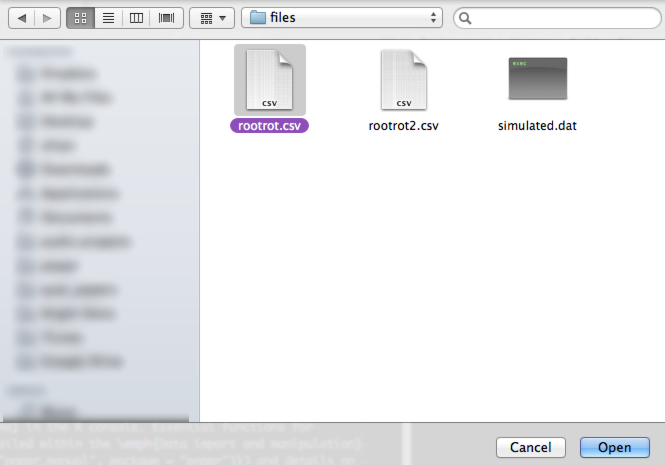
\includegraphics{getfile.png}
\end{figure}
\begin{center}
   \fcolorbox{black}{light-gray}{
        \begin{minipage}[t]{0.8\textwidth}
{\large \textsc{Hey! My window doesn't look like that!}}\\
Now, this window will not match up to your window on your computer because you will probably not be in the right directory. Remember the first path in \texttt{.libPaths()}? Move to a folder called \textbf{poppr} in that path. In that folder, you will find another folder called \textbf{files}. Move there and your window will match the one displayed.
        \end{minipage}
    }
\end{center}
\newpage

We can navigate throughout your entire computer through this little window and tell R where to go. The example I'm using goes to your R library directory. If you don't know where that is, you can find it by typing \texttt{.libPaths()} into the R command line.
Once we select a file, the file name and its path will be stored in the variable, x. We can confirm what we selected by simply typing \texttt{x} into R's command line.
\begin{Schunk}
\begin{Sinput}
> x
\end{Sinput}
\begin{Soutput}
$files
[1] "/path/to/R/poppr/files/rootrot.csv"

$path
[1] "/path/to/R/poppr/files"
\end{Soutput}
\end{Schunk}
Here we can see that \texttt{x} is a list with two entries: \texttt{\$files} giving you the files you selected and \texttt{\$path} giving you the path to those files. 
\begin{center}
   \fcolorbox{black}{light-gray}{
         \begin{minipage}[t]{0.8\textwidth}
{\large \textsc{Not sure what I mean by path or working directory?}}\\
For anyone who has never used a command line, this is a new concept. 
You can think of the path as an address. So instead of \texttt{"/path/to/R"}, you could have \texttt{"/USA/Oregon/Corvallis"}. Or on your computer, it could be \texttt{"C:/users/poppr-user/R/win-library/2.15"} on Windows (where "poppr-user" is your username) or \texttt{"/Library/Frameworks/R.framework/Versions/2.15/Resources/library"} on OSX. Each slash represents a folder that you would click through when you are using the mouse.

A working directory is simply the folder that R is working in. It is where you can access and write files. When you tell R to read a file, it will only look for that file in your working directory. Note that you will not endanger your files by reading them into R. R works by making a copy of the file into memory. This means that you can manipulate the data in any way that you want without ever losing the content.\\

To find out your current working directory, type \texttt{getwd()} into the R console. Usually, you will start off a session in your "home" directory, which will look like this: \texttt{"$\sim$/"}.
The command \texttt{setwd()} will change your working directory to any place of your choice on your computer as indicated by the path that you provide.
For more information, see Quick R at \url{http://www.statmethods.net}.
         \end{minipage}
      }
\end{center}

% Now we can set our working directory. That is, we can tell R to go to the folder that contains all of our data with the \texttt{setwd} command.
% <<setwd, eval=FALSE>>=
% setwd(x$path)
% @
We will use \texttt{x\$files} to access the file. The \texttt{poppr()} function provides a quick and convenient first analysis of your data directly from the file on the your disk (For information on importing your data into R, see section \ref{intro:import}, \textit{Get out of my dreams and into my R}).
\begin{Schunk}
\begin{Sinput}
> popdata <- poppr(x$files)
\end{Sinput}
\end{Schunk}
\begin{Schunk}
\begin{Soutput}
| Athena_1 
| Athena_2 
| Athena_3 
| Athena_4 
| Athena_5 
| Athena_6 
| Athena_7 
| Athena_8 
| Athena_9 
| Athena_10 
| Mt. Vernon_1 
| Mt. Vernon_2 
| Mt. Vernon_3 
| Mt. Vernon_4 
| Mt. Vernon_5 
| Mt. Vernon_6 
| Mt. Vernon_7 
| Mt. Vernon_8 
| Total 
\end{Soutput}
\end{Schunk}
The output of \texttt{poppr()} was assigned to the variable \texttt{popdata}, so let's look at the data.
\begin{Schunk}
\begin{Sinput}
> popdata
\end{Sinput}
\end{Schunk}
\begin{Schunk}
\begin{Soutput}
            Pop   N MLG   eMLG    SE     H      G  Hexp   E.5     Ia rbarD        File
1      Athena_1   9   7  7.000 0.000 1.889  6.231 0.944 0.932  2.925 0.210 rootrot.csv
2      Athena_2  12  12 10.000   NaN 2.485 12.000 1.000 1.000  4.160 0.128 rootrot.csv
3      Athena_3  10   2  2.000 0.000 0.325  1.220 0.200 0.571  2.000 1.000 rootrot.csv
4      Athena_4  13   9  7.154 0.769 1.946  5.121 0.872 0.687  5.495 0.372 rootrot.csv
5      Athena_5  10   7  7.000 0.000 1.834  5.556 0.911 0.866  4.532 0.353 rootrot.csv
6      Athena_6   5   5  5.000 0.000 1.609  5.000 1.000 1.000  2.464 0.190 rootrot.csv
7      Athena_7  11  10  9.182 0.386 2.272  9.308 0.982 0.955  2.129 0.086 rootrot.csv
8      Athena_8   8   6  6.000 0.000 1.667  4.571 0.893 0.831  3.857 0.323 rootrot.csv
9      Athena_9  10  10 10.000 0.000 2.303 10.000 1.000 1.000  2.815 0.118 rootrot.csv
10    Athena_10   9   8  8.000 0.000 2.043  7.364 0.972 0.948  2.849 0.137 rootrot.csv
11 Mt. Vernon_1  10   9  9.000 0.000 2.164  8.333 0.978 0.952  7.132 0.276 rootrot.csv
12 Mt. Vernon_2   6   6  6.000 0.000 1.792  6.000 1.000 1.000 20.649 0.492 rootrot.csv
13 Mt. Vernon_3   8   6  6.000 0.000 1.667  4.571 0.893 0.831  2.117 0.106 rootrot.csv
14 Mt. Vernon_4  12   8  6.833 0.665 1.814  4.500 0.848 0.681  3.008 0.255 rootrot.csv
15 Mt. Vernon_5  17   7  5.541 0.828 1.758  5.070 0.853 0.848  2.677 0.340 rootrot.csv
16 Mt. Vernon_6  12  11  9.318 0.466 2.369 10.286 0.985 0.958 19.498 0.467 rootrot.csv
17 Mt. Vernon_7  12   9  7.818 0.649 2.095  7.200 0.939 0.870  1.208 0.153 rootrot.csv
18 Mt. Vernon_8  13   9  7.346 0.764 2.032  6.259 0.910 0.794  1.153 0.169 rootrot.csv
19        Total 187 119  9.612 0.612 4.558 68.972 0.991 0.720 14.371 0.271 rootrot.csv
\end{Soutput}
\end{Schunk}
The fields you see in the output include:
\begin{itemize}
  \item \texttt{Pop -} Population name (Note that ``Total" also means ``Pooled").
  \item \texttt{N -} Number of individuals observed.
  \item \texttt{MLG -} Number of multilocus genotypes (MLG) observed.
  \item \texttt{eMLG -} The number of expected MLG at the smallest sample size $\geq 10$ based on rarefaction. \cite{Hurlbert:1971}
  \item \texttt{SE -} Standard error based on \texttt{eMLG} \cite{Heck:1975}
  \item \texttt{H -} Shannon-Wiener Index of MLG diversity. \cite{Shannon:1948}
  \item \texttt{G -} Stoddart and Taylor's Index of MLG diversity. \cite{Stoddart:1988}
  \item \texttt{Hexp -} Nei's 1978 genotypic diversity (corrected for sample size), or  Expected Heterozygosity. \cite{Nei:1978}
  \item \texttt{E.5 -} Evenness, $E_5$. \cite{Pielou:1975}\cite{Ludwig:1988}\cite{Grunwald:2003}
  \item \texttt{Ia -} The index of association, $I_A$. \cite{Brown:1980} \cite{Smith:1993} \cite{Agapow:2001}
  \item \texttt{rbarD -} The standardized index of association, $\bar r_d$. \cite{Agapow:2001}
\end{itemize}
These fields are further described in section \ref{summary}, \textit{I know what you did last summary table} at the end of this vignette. 

\subsection{Get out of my dreams and into my R \{importing data into poppr\}}\label{intro:import}
There are several ways of reading data into R. 
\subsubsection{Function: getfile}\label{intro:import:getfile}
\tab\tab \texttt{getfile} gives the user an easy way to point R to the directory in which your data is stored. It is only meant for R GUIs such as Rstudio. Using this on the command line has very little advantage over setting the working directory manually. 
\begin{quote}
Default Command:\\
\texttt{getfile(multi = FALSE, pattern = NULL, combine = TRUE)}
\end{quote}
\begin{itemize}
  \item \texttt{multi -} This is normally set to \texttt{FALSE}, meaning that it will only grab the file you selected. If it's \texttt{TRUE}, it will grab all files within the directory, constrained only by what you type into the \texttt{pattern} field.
  \item \texttt{pattern -} A pattern that you want to filter the files you get. This accepts regular expressions, so you must be careful with anything that is not an alphanumeric character.
  \item \texttt{combine -} This tells \texttt{getfile} to combine the path and all the files. This is set to \texttt{TRUE} by default so that you can access your files no matter what working directory you are in. 
\end{itemize}

This method works for a single file, but let's say you had a lot of data sets you wanted to import. You would have to do all of these one by one, right? Not so. \texttt{getfile} has a nice little flag called \texttt{multi} telling the computer that you want to grab multiple files in the folder. You would use this with \texttt{poppr.all} to produce a summary table for all of your files\footnote{These files do not need to be similar in any way to do this analysis}:
\begin{Schunk}
\begin{Sinput}
> x <- getfile(multi=TRUE)
\end{Sinput}
\end{Schunk}
A window would pop up again, and you should navigate to the same directory as you had before, and select any of the files in that directory. 
\begin{Schunk}
\begin{Sinput}
> x
\end{Sinput}
\end{Schunk}
\begin{Schunk}
\begin{Soutput}
$files
[1] "/path/to/R/poppr/files/rootrot.csv"   "/path/to/R/poppr/files/rootrot2.csv" 
[3] "/path/to/R/poppr/files/simulated.dat"

$path
[1] "/path/to/R/poppr/files"
\end{Soutput}
\end{Schunk}
As you can see, now all of the files that existed in that directory are there! Now you can look at all those files at once!
\begin{Schunk}
\begin{Sinput}
> poppr.all(x$files)
\end{Sinput}
\end{Schunk}
\begin{Schunk}
\begin{Soutput}
| File:  rootrot.csv 
| Athena_1 
| Athena_2 
| Athena_3 
| Athena_4 
| Athena_5 
| Athena_6 
| Athena_7 
| Athena_8 
| Athena_9 
| Athena_10 
| Mt. Vernon_1 
| Mt. Vernon_2 
| Mt. Vernon_3 
| Mt. Vernon_4 
| Mt. Vernon_5 
| Mt. Vernon_6 
| Mt. Vernon_7 
| Mt. Vernon_8 
| Total 
| File:  rootrot2.csv 
| 1 
| 2 
| 3 
| 4 
| 5 
| 6 
| 7 
| 8 
| 9 
| 10 
| Total 
| File:  simulated.dat 
| Total 
            Pop   N MLG   eMLG    SE     H      G  Hexp   E.5     Ia rbarD          File
1      Athena_1   9   7  7.000 0.000 1.889  6.231 0.944 0.932  2.925 0.210   rootrot.csv
2      Athena_2  12  12 10.000   NaN 2.485 12.000 1.000 1.000  4.160 0.128   rootrot.csv
3      Athena_3  10   2  2.000 0.000 0.325  1.220 0.200 0.571  2.000 1.000   rootrot.csv
4      Athena_4  13   9  7.154 0.769 1.946  5.121 0.872 0.687  5.495 0.372   rootrot.csv
5      Athena_5  10   7  7.000 0.000 1.834  5.556 0.911 0.866  4.532 0.353   rootrot.csv
6      Athena_6   5   5  5.000 0.000 1.609  5.000 1.000 1.000  2.464 0.190   rootrot.csv
7      Athena_7  11  10  9.182 0.386 2.272  9.308 0.982 0.955  2.129 0.086   rootrot.csv
8      Athena_8   8   6  6.000 0.000 1.667  4.571 0.893 0.831  3.857 0.323   rootrot.csv
9      Athena_9  10  10 10.000 0.000 2.303 10.000 1.000 1.000  2.815 0.118   rootrot.csv
10    Athena_10   9   8  8.000 0.000 2.043  7.364 0.972 0.948  2.849 0.137   rootrot.csv
11 Mt. Vernon_1  10   9  9.000 0.000 2.164  8.333 0.978 0.952  7.132 0.276   rootrot.csv
12 Mt. Vernon_2   6   6  6.000 0.000 1.792  6.000 1.000 1.000 20.649 0.492   rootrot.csv
13 Mt. Vernon_3   8   6  6.000 0.000 1.667  4.571 0.893 0.831  2.117 0.106   rootrot.csv
14 Mt. Vernon_4  12   8  6.833 0.665 1.814  4.500 0.848 0.681  3.008 0.255   rootrot.csv
15 Mt. Vernon_5  17   7  5.541 0.828 1.758  5.070 0.853 0.848  2.677 0.340   rootrot.csv
16 Mt. Vernon_6  12  11  9.318 0.466 2.369 10.286 0.985 0.958 19.498 0.467   rootrot.csv
17 Mt. Vernon_7  12   9  7.818 0.649 2.095  7.200 0.939 0.870  1.208 0.153   rootrot.csv
18 Mt. Vernon_8  13   9  7.346 0.764 2.032  6.259 0.910 0.794  1.153 0.169   rootrot.csv
19        Total 187 119  9.612 0.612 4.558 68.972 0.991 0.720 14.371 0.271   rootrot.csv
20            1  19  16  9.211 0.701 2.726 14.440 0.982 0.942 14.229 0.313  rootrot2.csv
21            2  18  18 10.000 0.000 2.890 18.000 1.000 1.000  9.143 0.194  rootrot2.csv
22            3  18   8  5.265 1.009 1.609  3.375 0.745 0.594 22.843 0.573  rootrot2.csv
23            4  25  17  7.887 1.124 2.575  9.615 0.933 0.710 18.488 0.415  rootrot2.csv
24            5  27  14  7.511 1.057 2.446  9.720 0.932 0.828 23.002 0.520  rootrot2.csv
25            6  17  15  9.338 0.633 2.670 13.762 0.985 0.949 17.778 0.410  rootrot2.csv
26            7  23  19  9.178 0.764 2.872 16.030 0.980 0.902 19.162 0.405  rootrot2.csv
27            8  21  15  8.273 0.981 2.558 10.756 0.952 0.820 24.313 0.543  rootrot2.csv
28            9  10  10 10.000 0.000 2.303 10.000 1.000 1.000  2.815 0.118  rootrot2.csv
29           10   9   8  8.000 0.000 2.043  7.364 0.972 0.948  2.849 0.137  rootrot2.csv
30        Total 187 119  9.612 0.612 4.558 68.972 0.991 0.720 14.371 0.271  rootrot2.csv
31        Total 100   6  6.000 0.000 1.235  2.790 0.648 0.735  0.050 0.061 simulated.dat
\end{Soutput}
\end{Schunk}

You've seen examples of how to use \texttt{getfile} to extract a single file and all the files in a directory, but what if you wanted many files, but only wanted ones that were of a certain type or had a certain name? This is what you would use the \texttt{pattern} argument for.
A perfect use would be the example data contained in the \textit{adegenet} package. Let's take a look at the names of these files.
\begin{center}
   \fcolorbox{black}{salmon}{
        \begin{minipage}[t]{0.8\textwidth}
         For the rest of this section, remember that every time you invoke \texttt{getfile()}, a window will pop up and you should select a file before hitting enter.
        \end{minipage}
      }
\end{center}
\begin{Schunk}
\begin{Sinput}
> getfile(multi=TRUE)
\end{Sinput}
\end{Schunk}
Navigate to the \textit{adegenet} folder in your R library.
\begin{Schunk}
\begin{Soutput}
$files
 [1] "/path/to/R/adegenet/files/AFLP.txt"         
 [2] "/path/to/R/adegenet/files/exampleSnpDat.snp"
 [3] "/path/to/R/adegenet/files/mondata1.rda"     
 [4] "/path/to/R/adegenet/files/mondata2.rda"     
 [5] "/path/to/R/adegenet/files/nancycats.dat"    
 [6] "/path/to/R/adegenet/files/nancycats.gen"    
 [7] "/path/to/R/adegenet/files/nancycats.gtx"    
 [8] "/path/to/R/adegenet/files/nancycats.str"    
 [9] "/path/to/R/adegenet/files/pdH1N1-data.csv"  
[10] "/path/to/R/adegenet/files/pdH1N1-HA.fasta"  
[11] "/path/to/R/adegenet/files/pdH1N1-NA.fasta"  
[12] "/path/to/R/adegenet/files/usflu.fasta"      

$path
[1] "/path/to/R/adegenet/files"
\end{Soutput}
\end{Schunk}

We can see that we have a mix of files with different formats. If we tried to run all of these files using poppr, we would have a problem because some of the file formats have no direct import into a \texttt{genind} object (*.fasta, or *.snp), or just simply are not supported (eg. *.rda files). We want to be able to filter these files out, and we will do so with the \texttt{pattern} argument. Let's say we only wanted the files that have the word "nancy" in them.
\begin{Schunk}
\begin{Sinput}
> getfile(multi=TRUE, pattern="nancy")
\end{Sinput}
\end{Schunk}
\begin{Schunk}
\begin{Soutput}
$files
[1] "/path/to/R/adegenet/files/nancycats.dat" "/path/to/R/adegenet/files/nancycats.gen"
[3] "/path/to/R/adegenet/files/nancycats.gtx" "/path/to/R/adegenet/files/nancycats.str"

$path
[1] "/path/to/R/adegenet/files"
\end{Soutput}
\end{Schunk}
Now, let's exclude everything but gentix files (*.gtx).
\begin{Schunk}
\begin{Sinput}
> getfile(multi=TRUE, pattern="gtx")
\end{Sinput}
\end{Schunk}
\begin{Schunk}
\begin{Soutput}
$files
[1] "/path/to/R/adegenet/files/nancycats.gtx"

$path
[1] "/path/to/R/adegenet/files"
\end{Soutput}
\end{Schunk}
Now, let's only get FSTAT files (*.dat)
\begin{Schunk}
\begin{Sinput}
> getfile(multi=TRUE, pattern="dat")
\end{Sinput}
\end{Schunk}
\begin{Schunk}
\begin{Soutput}
$files
[1] "/path/to/R/adegenet/files/mondata1.rda"   
[2] "/path/to/R/adegenet/files/mondata2.rda"   
[3] "/path/to/R/adegenet/files/nancycats.dat"  
[4] "/path/to/R/adegenet/files/pdH1N1-data.csv"

$path
[1] "/path/to/R/adegenet/files"
\end{Soutput}
\end{Schunk}

Uh-oh. We've run into a problem. Three out of our four files are not FSTAT files. Why did this happen? It happened because they happen to have \texttt{"dat"} within their name. This problem can be solved, by using regular expressions. If you are unfamiliar with regular expressions, you can think of them as special characters that you can use to make your search pattern more strict or more flexible. Since the topic of regular expressions can take up several lectures, I will spare you the gory details. For this situation, the only one you need to know is ``\texttt{\$}". The dollar sign indicates the end of a word or string. If we want specific file extensions all we have to do is add this to the end of the search term like so:
\begin{Schunk}
\begin{Sinput}
> getfile(multi=TRUE, pattern="dat$")
\end{Sinput}
\end{Schunk}
\begin{Schunk}
\begin{Soutput}
$files
[1] "/path/to/R/adegenet/files/nancycats.dat"

$path
[1] "/path/to/R/adegenet/files"
\end{Soutput}
\end{Schunk}
Now we have our FSTAT file!
\subsubsection{Function: read.genalex}\label{intro:import:read.genalex}

\tab\tab A very popular program for population genetics is GenAlEx (\url{http://biology.anu.edu.au/GenAlEx/Welcome.html}) \cite{Peakall:2012, Peakall:2006}. GenAlEx runs within the Excel environment and can be very powerful in its analyses. \textit{Poppr} has added the ability to read *.CSV files\footnote{*.CSV files are comma separated files that are easily machine readable.} produced in the GenAlEx format. It can handle data types containing regions and geographic coordinates, but currently it cannot import allelic frequency data from GenAlEx. All the user has to do is to export a single sheet of GenAlEx data from Excel into a *.CSV file, and the \textit{poppr} function \texttt{read.genalex} will import it into \textit{adegenet}'s \texttt{genind} object (more information on that below). For ways of formatting a GenAlEx file, see the manual here: \url{http://biology.anu.edu.au/GenAlEx/Download_files/GenAlEx\%206.5\%20Guide.pdf}
\begin{quote}
Default Command:\\
\texttt{read.genalex(genalex, ploidy = 2, geo = FALSE, region = FALSE)}
\end{quote}
\begin{itemize}
  \item \texttt{genalex -} a *.CSV file exported from GenAlEx on your disk (For example: \texttt{"my\_genalex\_file.csv"}).
  \item \texttt{ploidy -} a number indicating the ploidy for the data set (eg 2 for diploids, 1 for haploids).
  \item \texttt{geo -} GenAlEx allows you to have geographic data within your file. To do this for \textit{poppr}, you will need to follow the first format outlined in the GenAlEx manual and place the geographic data AFTER all genetic and demographic data with one blank column separating it (See the GenAlEx Manual for details). If you have geographic information in your file, set this flag to \texttt{TRUE} and it will be included within the resulting genind object in the \texttt{@other} slot. (If you don't know what that is, don't worry. It will be explained later in section \ref{intro:genind:other}).
  \item \texttt{region -} To format your GenAlEx file to include regions along with your populations, You can choose to include a separate column for regional data, or, since regional data must be in contiguous blocks, you can simply format it in the same way you would any other data (see the GenAlEx manual for details). If you have your file organized in this manner, select this option and the regional information will be stored in the resulting genind object in the \texttt{@other} slot.
\end{itemize}

\begin{center}
   \fcolorbox{black}{light-gray}{
         \begin{minipage}[t]{0.8\textwidth}
{\large \textsc{If you are unfamiliar with exporting data from Excel}}\\
\begin{enumerate}
  \item Click the Microsoft Office Button in the top left corner of Excel. (Or go to the File menu if you have an older version)
  \item Click Save As...
  \item In the ``Save as type" drop down box, select CSV (comma delimited). 
\end{enumerate}
        \end{minipage}
      }
\end{center}

Note that regional data and geographic data are not mutually exclusive. You can have both in one file, just make sure that they are on the same sheet and that the geographic data is always placed after all genetic and demographic data.

We have a short example of genalex formatted data with no geographic or regional formatting. We will first see where the data is using the command \texttt{system.file()}
\begin{Schunk}
\begin{Sinput}
> system.file("files/rootrot.csv", package="poppr")
\end{Sinput}
\end{Schunk}
\begin{Schunk}
\begin{Soutput}
[1] "/path/to/R/library/poppr/files/rootrot.csv"
\end{Soutput}
\end{Schunk}
Now import the data into \textit{poppr} like so:
\begin{Schunk}
\begin{Sinput}
> rootrot <- read.genalex(system.file("files/rootrot.csv", package="poppr"))
\end{Sinput}
\end{Schunk}
Executing rootrot shows that this file is now in genind format (ie. the format required by \textit{poppr} and \textit{adegenet}).
\begin{Schunk}
\begin{Sinput}
> rootrot
\end{Sinput}
\begin{Soutput}
   #####################
   ### Genind object ### 
   #####################
- genotypes of individuals - 

S4 class:  genind
@call: read.genalex(genalex = "rootrot.csv")

@tab:  187 x 56 matrix of genotypes

@ind.names: vector of  187 individual names
@loc.names: vector of  56 locus names
@loc.nall: NULL
@loc.fac: NULL
@all.names: NULL
@ploidy:  2
@type:  PA

Optionnal contents: 
@pop:  factor giving the population of each individual
@pop.names:  factor giving the population of each individual

@other: a list containing: population_hierarchy 
\end{Soutput}
\end{Schunk}

\subsubsection{Genalex formatting shortcuts}\label{intro:import:genalex.short}

\tab\tab The GenAlEx format is a nice way to import data because it allows you to have geographic coordinates and two hierarchical levels of sampling (Region and population). If you have multiple levels of hierarchy, you will need to code them so that you combine multiple columns of hierarchy into one using a common separator (For an example, see section \ref{data.manip:hier:splitcombine} of this manual). A problem arises when it becomes more work than it's worth to do that since, for the GenAlEx format, you must provide the sizes of each population in the header. Here, I'll show you a simple way to circumvent that. First, let's use the microbov data set from \textit{adegenet} (for details, type \texttt{help("microbov")} into your R console). It contains three demographic factors: Country, Species and Breed contained within the \texttt{@other} slot (detailed in section \ref{intro:genind:other}). We will combine these and save the file to our desktop. We will cover these functions later in this manual. For now, just know they exist.

\begin{Schunk}
\begin{Sinput}
> library(poppr)
> data(microbov)
> microbov@other$population_hierarchy <- data.frame(list(Country = microbov@other$coun, 
+   Species = microbov@other$spe, Breed = microbov@other$breed))
> microbov <- splitcombine(microbov, method=2, hier=c("Country", "Species", "Breed"))
> genind2genalex(microbov, file="~/Desktop/microbov.csv")
\end{Sinput}
\end{Schunk}
\begin{Schunk}
\begin{Soutput}
Extracting the table ... Writing the table to ~/Desktop/microbov.csv ... Done.
\end{Soutput}
\end{Schunk}
After we do this, we can open the file in our favorite spreadsheet editor and see the following image.

\setkeys{Gin}{width=\textwidth}

\begin{figure}[h!]
  \centering
  \caption{\footnotesize \footnotesize The first 15 individuals and 4 loci of the microbov data set. The first column contains the individual names, the second column contains the population names, and each subsequent column represents microsatellite genetic data. Highlighted in red is a list of populations and their relative sizes.}
  \label{microbov unmodified}
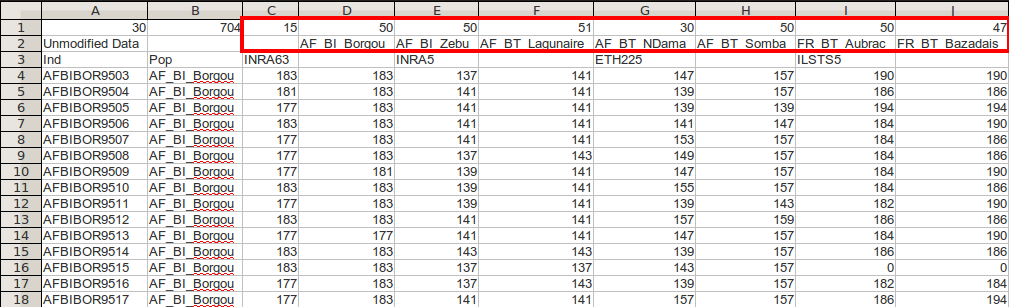
\includegraphics{unmod_dat}
\end{figure}

\newpage
All that \textit{poppr} needs from the first header row are the first three numbers (unless you are including regional data, but it's not terribly necessary with the hierarchical support \textit{poppr} provides.), which represent the number of loci, individuals, and populations, respectively. After that, you have counts of individuals per population in each subsequent cell. For \textit{poppr}, These cells don't matter because we already have that information in column 2.

If you have a large data set with many population levels, you can use the following shortcut by setting the number in the third cell to 1. The number in cell 4 is arbitrary (but must be there). In the following figure, it is set to the number of individuals in your data set, but can easily be replaced with any other number (perhaps your favorite number?). 

\begin{figure}[h!]
  \centering
  \caption{\footnotesize \footnotesize The first 15 individuals and 4 loci of the microbov data set. This is the same figure as above, however the populations and counts have been removed from the header row and the third number in the header has been replaced by 1.}
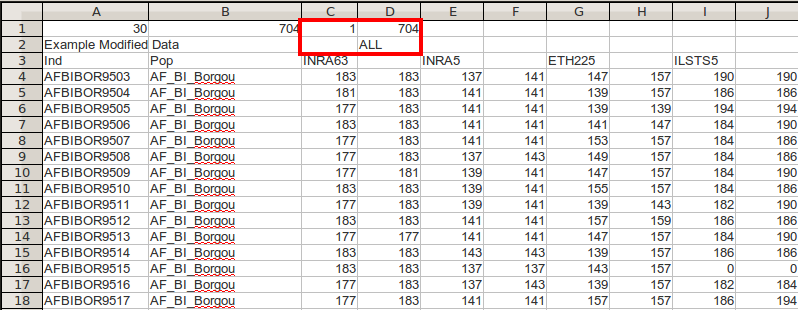
\includegraphics{mod_dat}
\end{figure}

\setkeys{Gin}{width=0.5\textwidth}

\subsubsection{Other ways of importing data}\label{intro:import:other}

\tab\tab \textit{Adegenet} already supports the import of FSTAT, Structure, Genpop, and Gentix formatted files, so if you have those formats, you can import them using the function \texttt{import2genind}. For sequence data, check if you can use \texttt{read.dna} from the \textit{ape} package to import your data. If you can, then you can use the \textit{adegenet} function \texttt{DNAbin2genind}. If you don't have any of these formats handy, you can still import your data using R's \texttt{read.table} along with \texttt{df2genind} from \textit{adegenet}. For more information, see \textit{adegenet}'s ``Getting Started" vignette.

\subsubsection{Function: genind2genalex}\label{intro:import:genind2genalex}

\tab\tab Of course, being able to export data is just as useful as being able to import it, so we have this handy little function that will write a GenAlEx formatted file to wherever you desire.\\ 
WARNING: This will overwrite any file that exists with the same name.
\begin{quote}
Default Command:\\
\texttt{genind2genalex(pop, filename = "genalex.csv", quiet = FALSE)}
\end{quote}
\begin{itemize}
  \item \texttt{pop -} a \texttt{genind} object.
  \item \texttt{filename -} This is where you specify where you want the file to go. If you simply type the file name, it will deposit the file in the directory R is currently in. If you don't know what directory you are in, you can type \texttt{getwd()} to find out.
  \item \texttt{quiet -} If this is set to \texttt{FALSE}, a message will be printed to the screen.
  \item \texttt{geo -} This is set to \texttt{FALSE} by default. If it is set to \texttt{TRUE}, then that means you have a data frame or matrix in the \texttt{@other} slot of your genind object that contains geographic coordinates for all individuals or all populations. Setting this to \texttt{TRUE} means that you want the resulting file to have two extra columns at the end of your file with geographic coordinates.
  \item \texttt{geodf -} The name of the data frame or matrix containing the geographic coordinates. The default is \texttt{geodf = "xy"}.
\end{itemize}

First, a simple example for the rootrot data we demonstrated in section 1.4.2:
\begin{Schunk}
\begin{Sinput}
> genind2genalex(rootrot, "~/Desktop/rootrot.csv")
\end{Sinput}
\end{Schunk}
\begin{Schunk}
\begin{Soutput}
Extracting the table ... Writing the table to ~/Desktop/rootrot.csv ... Done.
\end{Soutput}
\end{Schunk}

Now here's an example of exporting the nancycats data set into GenAlEx format with geographic information. If we look at the nancycats geographic information, we can see it's coordinates for each population, but not each individual:
\begin{Schunk}
\begin{Sinput}
> data(nancycats)
> nancycats@other$xy
\end{Sinput}
\begin{Soutput}
           x         y
P01 263.3498 171.10939
P02 183.5028 122.40790
P03 391.1050 254.70148
P04 458.6121  41.72336
P05 182.7769 219.08398
P06 335.2121 344.83557
P07 359.1662 375.36486
P08 271.3345  67.89132
P09 256.8169 150.02964
P10 270.6086  17.00917
P11 493.4544 237.25618
P12 305.4510  85.33663
P13 462.9674  86.79040
P14 429.5768 291.04587
P15 531.2003 115.13903
P16 407.8003  99.87438
P17 345.3745 251.79393
\end{Soutput}
\end{Schunk}
And we can export it easily:
\begin{Schunk}
\begin{Sinput}
> genind2genalex(nancycats, "~/Desktop/nancycats_pop_xy.csv")
\end{Sinput}
\end{Schunk}
\begin{Schunk}
\begin{Soutput}
Extracting the table ... Writing the table to ~/Desktop/nancycats_pop_xy.csv ... Done.
\end{Soutput}
\end{Schunk}
If we wanted to assign a geographic coordinate to each individual, we can simply use this little repetition trick knowing that there are 17 populations in the data set:
\begin{Schunk}
\begin{Sinput}
> nan2 <- nancycats
> nan2@other$xy <- nan2@other$xy[rep(1:17, table(pop(nan2))), ]
> head(nan2@other$xy)
\end{Sinput}
\begin{Soutput}
           x        y
P01 263.3498 171.1094
P01 263.3498 171.1094
P01 263.3498 171.1094
P01 263.3498 171.1094
P01 263.3498 171.1094
P01 263.3498 171.1094
\end{Soutput}
\end{Schunk}
Now we can export it to a different file.
\begin{Schunk}
\begin{Sinput}
> genind2genalex(nan2, "~/Desktop/nancycats_inds_xy.csv")
\end{Sinput}
\end{Schunk}
\begin{Schunk}
\begin{Soutput}
Extracting the table ... Writing the table to ~/Desktop/nancycats_inds_xy.csv ... Done.
\end{Soutput}
\end{Schunk}
%%%%%%%%%%%%%%%%%%%%%%%%%%%%%%%%%%%%%%%%%%%%%%%%%%%%%%%%%%%%%%%%%%%%%%%%%%%%%%%%
%%%%%%%%%%%%%%%%%%%%%%%%%%%%%%%%%%%%%%%%%%%%%%%%%%%%%%%%%%%%%%%%%%%%%%%%%%%%%%%%
%%%%%%%%%%%%%%%%%%%%%%%%%%%%%%%%%%%%%%%%%%%%%%%%%%%%%%%%%%%%%%%%%%%%%%%%%%%%%%%%
\subsection{Getting to know adegenet's genind object}\label{intro:genind}

\tab\tab Since \textit{poppr} was built around adegenet's framework, it is important to know how \textit{adegenet} stores data in the genind object, as that is the object used by \textit{poppr}. To create a genind object, \textit{adegenet} takes a data frame of genotypes (rows) across multiple loci (columns) and converts them into a matrix of individual allelic frequencies at each locus \cite{Jombart:2008}.

For example, if you had a data frame with 3 diploid individuals each with 3 loci that had 3, 4, and 5 allelic states respectively, the resulting \texttt{genind} object would contain a matrix that has 3 rows and 12 columns. 
\noindent Here's the example data frame:
\begin{Schunk}
\begin{Soutput}
   locus1  locus2  locus3
1 101/101 201/201 301/302
2 102/103 202/203 301/303
3 102/102 203/204 304/305
\end{Soutput}
\end{Schunk}
And the resulting matrix after importing to genind.
\begin{Schunk}
\begin{Soutput}
  L1.1 L1.2 L1.3 L2.1 L2.2 L2.3 L2.4 L3.1 L3.2 L3.3 L3.4 L3.5
1    1  0.0  0.0    1  0.0  0.0  0.0  0.5  0.5  0.0  0.0  0.0
2    0  0.5  0.5    0  0.5  0.5  0.0  0.5  0.0  0.5  0.0  0.0
3    0  1.0  0.0    0  0.0  0.5  0.5  0.0  0.0  0.0  0.5  0.5
\end{Soutput}
\end{Schunk}
The first three columns represent the alleles of locus 1, the next four represent locus 2, and the last five represent locus 3.

Do you see what I mean when I say individual allele frequencies at each locus? For a diploid individual, you only have three possible allele frequencies at each locus: 1, 0.5, or 0. Now, this is not the entire genind object, but it is the main feature. The object also has various elements associated with it that give you information about the population membership, the names of loci, individuals, and alleles among other things that \textit{poppr} uses to work \cite{Jombart:2008}. If you wish to know more, see the \textit{adegenet} ``Getting Started" manual. 

\subsubsection{The other slot}\label{intro:genind:other}

\tab\tab The element that you as a \textit{poppr} user needs to be concerned with is the ``other" slot. No, I'm not trying to be cryptic. If you look at an \textit{adegenet} object, you will see that it has several ``slots" (starting with ``@"). \cite{Jombart:2008} Let's start by recreating that data frame I showed you earlier.
\begin{Schunk}
\begin{Sinput}
> df <- data.frame(list(locus1=c("101/101", "102/103", "102/102"), 
+                       locus2=c("201/201", "202/203", "203/204"), 
+                       locus3=c("301/302", "301/303", "304/305")
+                       )
+                  )
> dfg <- df2genind(df, sep="/")
\end{Sinput}
\end{Schunk}
Next we will display the contents of the \texttt{genind} object \texttt{dfg}
\begin{Schunk}
\begin{Sinput}
> dfg
\end{Sinput}
\begin{Soutput}
   #####################
   ### Genind object ### 
   #####################
- genotypes of individuals - 

S4 class:  genind
@call: df2genind(X = df, sep = "/")

@tab:  3 x 12 matrix of genotypes

@ind.names: vector of  3 individual names
@loc.names: vector of  3 locus names
@loc.nall: number of alleles per locus
@loc.fac: locus factor for the  12 columns of @tab
@all.names: list of  3 components yielding allele names for each locus
@ploidy:  2
@type:  codom

Optionnal contents: 
@pop:  - empty -
@pop.names:  - empty -

@other: - empty -
\end{Soutput}
\end{Schunk}

The matrix containing our allelic frequencies is located in the \texttt{@tab} slot. All of the  slots below that have very specific properties related to the matrix in \texttt{@tab}, but the \texttt{@other} slot is more or less a grab bag, where you can place anything you want, even if it doesn't make sense!

Here, I'll give you an example of placing the genind object inside itself. Notice first, that the \texttt{@other} slot is empty and pay attention to the commands I use, noting that you can use either ``\$" or ``@" to access the slots.
\begin{Schunk}
\begin{Sinput}
> # First off, how big is the object?
> print(object.size(dfg), units="auto")
\end{Sinput}
\begin{Soutput}
8.5 Kb
\end{Soutput}
\begin{Sinput}
> dfg$other$dfg <- dfg
> dfg # we can now see that the @other slot is now filled.
\end{Sinput}
\begin{Soutput}
   #####################
   ### Genind object ### 
   #####################
- genotypes of individuals - 

S4 class:  genind
@call: df2genind(X = df, sep = "/")

@tab:  3 x 12 matrix of genotypes

@ind.names: vector of  3 individual names
@loc.names: vector of  3 locus names
@loc.nall: number of alleles per locus
@loc.fac: locus factor for the  12 columns of @tab
@all.names: list of  3 components yielding allele names for each locus
@ploidy:  2
@type:  codom

Optionnal contents: 
@pop:  - empty -
@pop.names:  - empty -

@other: a list containing: dfg 
\end{Soutput}
\begin{Sinput}
> dfg$other$dfg
\end{Sinput}
\begin{Soutput}
   #####################
   ### Genind object ### 
   #####################
- genotypes of individuals - 

S4 class:  genind
@call: df2genind(X = df, sep = "/")

@tab:  3 x 12 matrix of genotypes

@ind.names: vector of  3 individual names
@loc.names: vector of  3 locus names
@loc.nall: number of alleles per locus
@loc.fac: locus factor for the  12 columns of @tab
@all.names: list of  3 components yielding allele names for each locus
@ploidy:  2
@type:  codom

Optionnal contents: 
@pop:  - empty -
@pop.names:  - empty -

@other: - empty -
\end{Soutput}
\begin{Sinput}
> print(object.size(dfg), units="auto") # How big is it now?
\end{Sinput}
\begin{Soutput}
17.2 Kb
\end{Soutput}
\end{Schunk}
\begin{center}
   \fcolorbox{black}{light-gray}{
         \begin{minipage}[t]{0.8\textwidth}
{\large \textsc{What is the \# sign for?}}\\
This is called a comment. If you type something in R with the ``\#" sign in front of it, R will not interpret it.
        \end{minipage}
      }
\end{center}

And we can continue to do this until we reach the limit of our available memory. Why am I showing this silliness to you? For one thing I want to show you that you can stick anything you want into that slot and the object will not be hurt in any way. It's also important when considering how you are going to deal with the population structure of your genind object. For the \textit{poppr} functions \texttt{clonecorrect} (Section \ref{data.manip:cc:clonecorrect}) and \texttt{splitcombine} (Section \ref{data.manip:hier:splitcombine}) to work, a data frame of the population hierarchy must be present in the \texttt{@other} slot and it must have the same number of rows as individuals in the data set. There are several ways to go about this. If you know how to create a data frame or import data into R, the command is no more difficult than \texttt{obj\$other\$population\_hierarchy <- df}. If you do not know how to create a data frame or import data into R, you can visit Quick R at \url{http://www.statmethods.net/input/importingdata.html}.
\subsubsection{Setting the population factor \{adegenet's function: pop\}}\label{intro:genind:pop}

\tab\tab A genind object can contain several populations, and, if you have differing population structures, you might want to switch among them for different analyses. The tools you as the user would need, are the slot \texttt{@pop.names} and the \textit{adegenet} function \texttt{pop()}. I'll use the H3N2 data set packaged with \textit{adegenet} as an example.
\begin{Schunk}
\begin{Sinput}
> data(H3N2)
> H3N2
\end{Sinput}
\begin{Soutput}
   #####################
   ### Genind object ### 
   #####################
- genotypes of individuals - 

S4 class:  genind
@call: .local(x = x, i = i, j = j, drop = drop)

@tab:  1903 x 334 matrix of genotypes

@ind.names: vector of  1903 individual names
@loc.names: vector of  125 locus names
@loc.nall: number of alleles per locus
@loc.fac: locus factor for the  334 columns of @tab
@all.names: list of  125 components yielding allele names for each locus
@ploidy:  1
@type:  codom

Optionnal contents: 
@pop:  - empty -
@pop.names:  - empty -

@other: a list containing: x  xy  epid 
\end{Soutput}
\begin{Sinput}
> pop(H3N2)
\end{Sinput}
\begin{Soutput}
NULL
\end{Soutput}
\begin{Sinput}
> H3N2$pop.names
\end{Sinput}
\begin{Soutput}
NULL
\end{Soutput}
\end{Schunk}

Notice how both the pop and pop.names are empty. This means that the population information needs to be set. Notice, however that there are 1903 individuals in the data set and that the \texttt{@other} slot is not empty. Let's investigate an object in this slot.
\begin{Schunk}
\begin{Sinput}
> head(H3N2$other$x)
\end{Sinput}
\begin{Soutput}
         accession length  host segment subtype country year       Virus name
AB434107  AB434107   1701 Human  4 (HA)    H3N2   Japan 2002 Influenza Avirus
AB434108  AB434108   1701 Human  4 (HA)    H3N2   Japan 2002 Influenza Avirus
AB438242  AB438242    827 Human  4 (HA)    H3N2   Japan 2002 Influenza Avirus
AB438243  AB438243    827 Human  4 (HA)    H3N2   Japan 2002 Influenza Avirus
AB438244  AB438244    827 Human  4 (HA)    H3N2   Japan 2002 Influenza Avirus
AB438245  AB438245    827 Human  4 (HA)    H3N2   Japan 2002 Influenza Avirus
                           Misc info  Age Gender       date usePreciseLoc localisation
AB434107   (A/Morioka/34/2002(H3N2)) <NA>   <NA> 2002/02/25         FALSE        japan
AB434108   (A/Morioka/52/2002(H3N2)) <NA>   <NA> 2002/03/01         FALSE        japan
AB438242  (A/Niigata/F11/2002(H3N2)) <NA>   <NA> 2002/01/22         FALSE        japan
AB438243 (A/Niigata/F100/2002(H3N2)) <NA>   <NA> 2002/02/18         FALSE        japan
AB438244 (A/Niigata/F175/2002(H3N2)) <NA>   <NA> 2002/02/25         FALSE        japan
AB438245 (A/Niigata/F245/2002(H3N2)) <NA>   <NA> 2002/03/04         FALSE        japan
              lon      lat month
AB434107 137.2155 35.58418     2
AB434108 137.2155 35.58418     3
AB438242 137.2155 35.58418     1
AB438243 137.2155 35.58418     2
AB438244 137.2155 35.58418     2
AB438245 137.2155 35.58418     3
\end{Soutput}
\begin{Sinput}
> nrow(H3N2$other$x)
\end{Sinput}
\begin{Soutput}
[1] 1903
\end{Soutput}
\end{Schunk}
\begin{center}
   \fcolorbox{black}{light-gray}{
        \begin{minipage}[t]{0.8\textwidth}
{\large \textsc{What is head()?}}\\
\texttt{head()} is a command that will show you only the top portion of an R object. By default it will show you the first six elements (or rows of a data frame or matrix). This is so that you can quickly check the contents of an object.
        \end{minipage}
   }
\end{center}

We can see that it's a data frame containing a wealth of information that we could use to subset our data. So, let's start by setting the population structure by country. How do we do that? Well, the function \texttt{pop()} will allow us to set that structure using a vector that is the same length as the number of individuals in the data set. Since the number of rows in the data frame \texttt{x} meets that criteria, we can use any item in that data frame. Let's take a look.
\begin{Schunk}
\begin{Sinput}
> pop(H3N2) <- H3N2$other$x$country
> head(pop(H3N2))
\end{Sinput}
\begin{Soutput}
[1] Japan Japan Japan Japan Japan Japan
37 Levels: Japan USA Finland China South Korea Norway Taiwan France ... Algeria
\end{Soutput}
\begin{Sinput}
> H3N2$pop.names
\end{Sinput}
\begin{Soutput}
 [1] "Japan"          "USA"            "Finland"        "China"          "South Korea"   
 [6] "Norway"         "Taiwan"         "France"         "Latvia"         "Netherlands"   
[11] "Bulgaria"       "Turkey"         "United Kingdom" "Denmark"        "Austria"       
[16] "Canada"         "Italy"          "Russia"         "Bangladesh"     "Egypt"         
[21] "Germany"        "Romania"        "Ukraine"        "Czech Republic" "Greece"        
[26] "Iceland"        "Ireland"        "Sweden"         "Nepal"          "Saudi Arabia"  
[31] "Switzerland"    "Iran"           "Mongolia"       "Spain"          "Slovenia"      
[36] "Croatia"        "Algeria"       
\end{Soutput}
\end{Schunk}
Notice how useful the \texttt{@other} slot can be. We now have population structure in the data set and you now know how to set the population factor. The other slot will become useful later on when we are talking about multilocus genotypes.
%%%%%%%%%%%%%%%%%%%%%%%%%%%%%%%%%%%%%%%%%%%%%%%%%%%%%%%%%%%%%%%%%%%%%%%%%%%%%%%%
%
%%%%%%%%%%%%%%%%%%%%%%%%%%%%%%%%%%%%%%%%%%%%%%%%%%%%%%%%%%%%%%%%%%%%%%%%%%%%%%%%
%
%%%%%%%%%%%%%%%%%%%%%%%%%%%%%%%%%%%%%%%%%%%%%%%%%%%%%%%%%%%%%%%%%%%%%%%%%%%%%%%%
%
%%%%%%%%%%%%%%%%%%%%%%%%%%%%%%%%%%%%%%%%%%%%%%%%%%%%%%%%%%%%%%%%%%%%%%%%%%%%%%%%
\section{Data Manipulation}\label{data.manip}

\tab\tab One tedious aspect of population genetic analysis is the need for repeated data manipulation. \textit{Adegenet} has some functions for manipulating data that are limited to replacing missing data and dividing data into populations, loci, or by sample size \cite{Jombart:2008}. \textit{Poppr} includes novel functions for clone-censoring your data sets or sub-setting a genind object by specific populations.
%%%%%%%%%%%%%%%%%%%%%%%%%%%%%%%%%%%%%%%%%%%%%%%%%%%%%%%%%%%%%%%%%%%%%%%%%%%%%%%%
%%%%%%%%%%%%%%%%%%%%%%%%%%%%%%%%%%%%%%%%%%%%%%%%%%%%%%%%%%%%%%%%%%%%%%%%%%%%%%%%
%%%%%%%%%%%%%%%%%%%%%%%%%%%%%%%%%%%%%%%%%%%%%%%%%%%%%%%%%%%%%%%%%%%%%%%%%%%%%%%%
\subsection{Inside the golden days of missing data \{replace or remove missing data\}}\label{data.manip:missing}

\tab\tab A data set without missing data is always ideal, but often not achievable. Many functions in \textit{adegenet} cannot handle missing data and thus the function \texttt{na.replace} exists \cite{Jombart:2008}. It will replace missing data with with either ``0" representing a mysterious extra allele in the data set resulting in more diversity or the mean of allelic frequencies at the locus. There is no set method, however, for simply removing missing data from analyses, which is why the \textit{poppr} function \texttt{missingno} (see below) exists. If the name makes you uneasy it's because it should. Missing data can mean different things based on your data type. For microsatellites, missing data might represent any source of error that could cause a PCR product to not amplify in gel electrophoresis, which may or may not be biologically relevant. For a DNA alignment, missing data could mean something as simple as an insertion or deletion, which is biologically relevant. The choice to exclude or estimate data has very different implications for the type of data you have.
\subsubsection{Function: missingno}\label{data.manip:missing:missingno}

\tab\tab \texttt{missingno} is a function that serves partially as a wrapper for adegenet's \texttt{na.replace} to replace missing data and as a way to exclude specific areas that contain systematic missing data.  
\begin{quote}
Default Command:\\
\texttt{missingno(pop, type = "loci", cutoff = 0.05, quiet = FALSE)}
\end{quote}
\begin{itemize}
  \item \texttt{pop -} a \texttt{genind} object.
  \item \texttt{type -} This could be one of four options:
    \begin{description}
      \item[ ``mean"] This replaces missing data with the mean allele frequencies in the entire data set.
      \item[ ``zero" or ``0"] This replaces missing data with zero, signifying a new allele.
      \item[ ``loci"] This is to be used for a data set that has systematic problems with certain loci that contain null alleles or simply failed to amplify. This will remove loci with a defined threshold of missing data from the data set.
      \item[ ``geno"] This is to be used for genotypes (individuals) in your data set where many null alleles are present. Individuals with a defined threshold missing data will be removed.
    \end{description}
    \item \texttt{cutoff -} This is a numeric value from 0 to 1 indicating the percent allowable missing data for either loci or genotypes. If you have, for example, two loci containing missing 5\% and 10\% missing data, respectively and you set \texttt{cutoff = 0.05}, \texttt{missingno} will remove the second locus. Percent missing data for genotypes is considered the percent missing loci over number of total loci. 
    \item \texttt{quiet -} When this is set to \texttt{FALSE}, the number of missing values replaced will be printed to screen if the method is ``zero" or ``mean". It will print the number of loci or individuals removed if the method is ``loci" or ``geno".
\end{itemize}

Of course, seeing is believing. Let's take a look at what this does by focusing in on areas with missing data. Note that I will be using some sub-setting functions here that are described in adegenet's \textit{Getting Started} vignette. First, let's take a look at what the missing data in R looks like as well as how many loci and individuals the data set nancycats contains. We need to first tell R to look in its library for the package \textit{poppr}.
\begin{Schunk}
\begin{Sinput}
> library(poppr)
\end{Sinput}
\end{Schunk}
Next, we'll initialize the \textit{adegenet} data set nancycats and load it into memory.
\begin{Schunk}
\begin{Sinput}
> data(nancycats)
\end{Sinput}
\end{Schunk}
Now, we'll take a quick look at the nancycats data set using \textit{adegenet}'s \texttt{summary()} \index{summary} function:
\begin{Schunk}
\begin{Sinput}
> summary(nancycats)
\end{Sinput}
\begin{Soutput}
 # Total number of genotypes:  237 

 # Population sample sizes:  
 1  2  3  4  5  6  7  8  9 10 11 12 13 14 15 16 17 
10 22 12 23 15 11 14 10  9 11 20 14 13 17 11 12 13 

 # Number of alleles per locus:  
L1 L2 L3 L4 L5 L6 L7 L8 L9 
16 11 10  9 12  8 12 12 18 

 # Number of alleles per population:  
01 02 03 04 05 06 07 08 09 10 11 12 13 14 15 16 17 
36 53 50 67 48 56 42 54 43 46 70 52 44 61 42 40 35 

 # Percentage of missing data:  
[1] 2.344116

 # Observed heterozygosity:  
       L1        L2        L3        L4        L5        L6        L7        L8        L9 
0.6682028 0.6666667 0.6793249 0.7083333 0.6329114 0.5654008 0.6497890 0.6184211 0.4514768 

 # Expected heterozygosity:  
       L1        L2        L3        L4        L5        L6        L7        L8        L9 
0.8657224 0.7928751 0.7953319 0.7603095 0.8702576 0.6884669 0.8157881 0.7603493 0.6062686 
\end{Soutput}
\end{Schunk}

We can see here a lot of summary statistics about nancycats. Here we can see that there are 17 populations, 237 individuals, and 9 loci. Nancycats also has a little over 2.3\% missing data. Let's take a look at the names of the loci and the structure of the data. In order to save space, I will only show you the first five individuals (rows) and a portion of the alleles in the first locus (columns).
\begin{Schunk}
\begin{Sinput}
> nancycats$loc.names # Names of the loci
\end{Sinput}
\begin{Soutput}
     L1      L2      L3      L4      L5      L6      L7      L8      L9 
 "fca8" "fca23" "fca43" "fca45" "fca77" "fca78" "fca90" "fca96" "fca37" 
\end{Soutput}
\begin{Sinput}
> nancycats$tab[1:5, 8:13]
\end{Sinput}
\begin{Soutput}
    L1.08 L1.09 L1.10 L1.11 L1.12 L1.13
001    NA    NA    NA    NA    NA    NA
002    NA    NA    NA    NA    NA    NA
003   0.0   0.5     0     0     0   0.5
004   0.5   0.5     0     0     0   0.0
005   0.5   0.5     0     0     0   0.0
\end{Soutput}
\end{Schunk}

When looking at this data set, recall how a \texttt{genind} object is formatted. You have a matrix of 0's, 1's and 0.5's. For diploids, if you see 0.5, that means it is heterozygous at that allele, and a 1 means it's homozygous. Here we see three heterozygotes and two individuals with missing data (indicated by NA). Now, there are more places with missing data in the data set, but I'm only showing a little bit at one locus so it's easier to digest. Let's first replace it by zero and mean, respectively.
\begin{Schunk}
\begin{Sinput}
> nanzero <- missingno(nancycats, type = "zero")
\end{Sinput}
\begin{Soutput}
 Replaced 617 missing values 
\end{Soutput}
\begin{Sinput}
> nanmean <- missingno(nancycats, type = "mean")
\end{Sinput}
\begin{Soutput}
 Replaced 617 missing values 
\end{Soutput}
\begin{Sinput}
> nanzero$tab[1:5, 8:13]
\end{Sinput}
\begin{Soutput}
    L1.08 L1.09 L1.10 L1.11 L1.12 L1.13
001   0.0   0.0     0     0     0   0.0
002   0.0   0.0     0     0     0   0.0
003   0.0   0.5     0     0     0   0.5
004   0.5   0.5     0     0     0   0.0
005   0.5   0.5     0     0     0   0.0
\end{Soutput}
\begin{Sinput}
> nanmean$tab[1:5, 8:13]
\end{Sinput}
\begin{Soutput}
         L1.08     L1.09     L1.10      L1.11      L1.12     L1.13
001 0.07603687 0.2419355 0.1912442 0.06221198 0.09447005 0.1013825
002 0.07603687 0.2419355 0.1912442 0.06221198 0.09447005 0.1013825
003 0.00000000 0.5000000 0.0000000 0.00000000 0.00000000 0.5000000
004 0.50000000 0.5000000 0.0000000 0.00000000 0.00000000 0.0000000
005 0.50000000 0.5000000 0.0000000 0.00000000 0.00000000 0.0000000
\end{Soutput}
\end{Schunk}
You notice how the values of NA changed, yet the basic structure stayed the same. These are the replacement options from adegenet. Let's look at the same example with the exclusion options (set to the default cutoff of 5\%).
\begin{Schunk}
\begin{Sinput}
> nanloci <-  missingno(nancycats, "loci")
\end{Sinput}
\begin{Soutput}
 Found 617 missing values.
 2 loci contained missing values greater than 5%.
 Removing 2 loci : fca8 fca45 
\end{Soutput}
\begin{Sinput}
> nangeno <-  missingno(nancycats, "geno")
\end{Sinput}
\begin{Soutput}
 Found 617 missing values.
 38 genotypes contained missing values greater than 5%.
 Removing 38 genotypes : N215 N216 N188 N189 N190 N191 N192 N302 N304 N310 
N195 N197 N198 N199 N200 N201 N206 N182 N184 N186 N298 N299 N300 N301 N303 N282 
N283 N288 N291 N292 N293 N294 N295 N296 N297 N281 N289 N290 
\end{Soutput}
\begin{Sinput}
> nanloci$tab[1:5, 8:13]
\end{Sinput}
\begin{Soutput}
    L1.08 L1.09 L1.10 L1.11 L2.01 L2.02
001     0   0.5     0     0     0     0
002     0   1.0     0     0     0     0
003     0   0.5     0     0     0     0
004     0   0.0     0     0     0     0
005     0   0.5     0     0     0     0
\end{Soutput}
\end{Schunk}

Notice how we now see columns named ``L2.01" and ``L2.02". This is showing us another locus because we have removed the first. Recall from the summary table that the first locus had 16 alleles, and the second had 11. Now that we've removed loci containing missing data, all others have shifted over.\\
Let's look at the loci names and number of individuals.
\begin{Schunk}
\begin{Sinput}
> length(nanloci$ind.names) # Individuals
\end{Sinput}
\begin{Soutput}
[1] 237
\end{Soutput}
\begin{Sinput}
> nanloci$loc.names # Names of the loci
\end{Sinput}
\begin{Soutput}
     L1      L2      L3      L4      L5      L6      L7 
"fca23" "fca43" "fca77" "fca78" "fca90" "fca96" "fca37" 
\end{Soutput}
\end{Schunk}
You can see that the number of individuals stayed the same but the loci ``fca8", ``fca45", and ``fca96" were removed.\\
Let's look at what happened when we removed individuals.
\begin{Schunk}
\begin{Sinput}
> nangeno$tab[1:5, 8:13]
\end{Sinput}
\begin{Soutput}
    L1.08 L1.09 L1.10 L1.11 L1.12 L1.13
001   0.0   0.5     0     0     0   0.5
002   0.5   0.5     0     0     0   0.0
003   0.5   0.5     0     0     0   0.0
004   0.0   0.5     0     0     0   0.5
005   0.0   1.0     0     0     0   0.0
\end{Soutput}
\begin{Sinput}
> length(nangeno$ind.names) # Individuals
\end{Sinput}
\begin{Soutput}
[1] 199
\end{Soutput}
\begin{Sinput}
> nangeno$loc.names # Names of the loci
\end{Sinput}
\begin{Soutput}
     L1      L2      L3      L4      L5      L6      L7      L8      L9 
 "fca8" "fca23" "fca43" "fca45" "fca77" "fca78" "fca90" "fca96" "fca37" 
\end{Soutput}
\end{Schunk}

We can see here that the number of individuals decreased, yet we have the same number of loci. Notice how the frequency matrix changes in both scenarios? In the scenario with ``loci", we removed several columns of the data set, and so with our sub-setting, we see alleles from the second locus. In the scenario with ``geno", we removed several rows of the data set so we see other individuals in our sub-setting.
%%%%%%%%%%%%%%%%%%%%%%%%%%%%%%%%%%%%%%%%%%%%%%%%%%%%%%%%%%%%%%%%%%%%%%%%%%%%%%%%
%%%%%%%%%%%%%%%%%%%%%%%%%%%%%%%%%%%%%%%%%%%%%%%%%%%%%%%%%%%%%%%%%%%%%%%%%%%%%%%%
%%%%%%%%%%%%%%%%%%%%%%%%%%%%%%%%%%%%%%%%%%%%%%%%%%%%%%%%%%%%%%%%%%%%%%%%%%%%%%%%
\subsection{Can you take me hier(archy)? \{population hierarchy construction\}}\label{data.manip:hier}

\tab\tab Remember all that fuss we made about the \texttt{@other} slot above in section \ref{intro:genind:other}? The way you can achieve hierarchical analysis in \textit{poppr} is through a data frame in that slot. Many of the file formats that \textit{adegenet} and \textit{poppr} can import do not allow for more than two hierarchies. If you need more levels, you have a couple of choices: 
\begin{enumerate}
  \item Import them into R as a data frame with each column being a separate hierarchical element.
  \item Collapse them into a single population factor so that you can trick these file formats into taking multiple population hierarchies (eg. instead of ``Pop1", ``Subpop1", ``Subsubpop1", you would have ``Pop1\_Subpop1\_Subsubpop1"). 
\end{enumerate}
Whichever choice you make, The \textit{poppr} function \texttt{splitcombine} can help you divide and combine those factors in any way you can think of.
\subsubsection{Function: splitcombine}\label{data.manip:hier:splitcombine}

\tab\tab This function will allow you to combine your population hierarchies in ways meaningful to your data without needing to know R programming. It can either split a vector of combined population hierarchies or it can combine columns of a data frame containing population hierarchies (Note that it will only split the first column of the data frame if you choose \texttt{method = 1}).
\begin{quote}
Default Command:\\
\texttt{splitcombine(pop, method = 1, dfname = "population\_hierarchy", sep = "\_", hier = c(1), setpopulation = TRUE, fixed = TRUE)}
\end{quote}
\begin{itemize}
  \item \texttt{pop -} a \texttt{genind} object with a data frame in the \texttt{@other} slot.
  \item \texttt{method -} An integer indicating what you want to do on your data frame:
  \begin{enumerate}
    \item \textbf{split} Any populations combined using a common separator in your data frame. So, a population hierarchy of ``Pop1\_Subpop1\_Subsubpop1" would be split into a data frame containing the columns ``Pop1", ``Subpop1", ``Subsubpop1". Since it will split the population factor, it needs only to be used once. 
    \item \textbf{combine} If you have your population hierarchy split into a data frame, you can do the exact opposite of method 1 and combine separate elements into one.
  \end{enumerate}
  \item \texttt{dfname -} This is the name of the data frame containing your population factor. Note that you are not limited to one data frame in your genind object. If you do not have that data frame in the \texttt{@other} slot, a warning will be returned and nothing will happen.
  \item \texttt{sep -} A separation factor you want to separate your populations with. Note, that you can choose whatever you want, but be careful because some characters have special meanings (regular expressions) in R and could give you incorrect results (``\_" is the suggested default).
  \item \texttt{hier -} This can be a vector of words or numbers referring to what you want to name your population hierarchies in \texttt{method = 1}, or specific column names in your data frame in \texttt{method = 2}. 
  \item \texttt{setpopulation -} if \texttt{TRUE} (default), this will automatically set the population factor to either the highest population factor (with \texttt{method = 1}, split) or the combined population hierarchy (with \texttt{method = 2}, combine). if this is set to \texttt{FALSE}, the population factor will not be set.
  \item \texttt{fixed -} This is an option to be passed onto the \textit{base} function \texttt{strsplit}. For those not familiar with regular expressions, it will tell R whether or not the character in \texttt{split} should be treated as a special character or not. If you don't know regular expressions, don't touch it.
\end{itemize}

Let's give an example using AFLP data of different populations of \textit{A. euteiches} collected in Washington and Oregon. \cite{Grunwald:2006}
\begin{Schunk}
\begin{Sinput}
> Aeut <- read.genalex(system.file("files/rootrot.csv", package="poppr"))
> summary(Aeut)
\end{Sinput}
\begin{Soutput}
 # Total number of genotypes:  187 

 # Population sample sizes:  
    Athena_1     Athena_2     Athena_3     Athena_4     Athena_5     Athena_6 
           9           12           10           13           10            5 
    Athena_7     Athena_8     Athena_9    Athena_10 Mt. Vernon_1 Mt. Vernon_2 
          11            8           10            9           10            6 
Mt. Vernon_3 Mt. Vernon_4 Mt. Vernon_5 Mt. Vernon_6 Mt. Vernon_7 Mt. Vernon_8 
           8           12           17           12           12           13 

 # Percentage of missing data:  
[1] 0
\end{Soutput}
\end{Schunk}
\begin{center}
   \fcolorbox{black}{light-gray}{
         \begin{minipage}[t]{0.8\textwidth}
{\large \textsc{Does this summary seem a little lacking?}}\\
The data that we have here is presence absence data. This means that many of the functions that \textit{adegenet} uses to calculate heterozygosity and number of alleles are slightly useless in this regard.
        \end{minipage}
      }
\end{center}
Notice that we have 18 different ``populations" here, but they are really a hierarchy. Let's say we want to analyze the diversity statistics of the two overall populations. Take a look at how the combined population factor is kept in the data frame.
\begin{Schunk}
\begin{Sinput}
> head(Aeut$other$population_hierarchy)
\end{Sinput}
\begin{Soutput}
       Pop
1 Athena_1
2 Athena_1
3 Athena_1
4 Athena_1
5 Athena_1
6 Athena_1
\end{Soutput}
\end{Schunk}
We'll use \texttt{splitcombine} to split that into a population and sub-population and set the population factor to the population.
\begin{center}
   \fcolorbox{black}{light-gray}{
         \begin{minipage}[t]{0.8\textwidth}
{\large \textsc{Important point about splitcombine}}\\
Ideally, method split should only be used once after you read in your data. The reason for this is that when you select this method, it will look in the first column of your data frame to choose the combined population factor to split.
If you do not name your hierarchy or if you attempt to give your hierarchy too many names, it will automatically name the columns ``h1", ``h2", etc. 
        \end{minipage}
      }
\end{center}
\begin{Schunk}
\begin{Sinput}
> Aeut.pop <- splitcombine(Aeut, method=1, dfname="population_hierarchy", hier=c("Pop", "Subpop"), setpopulation=TRUE)
> head(Aeut.pop$other$population_hierarchy)
\end{Sinput}
\begin{Soutput}
  Pop_Subpop    Pop Subpop
1   Athena_1 Athena      1
2   Athena_1 Athena      1
3   Athena_1 Athena      1
4   Athena_1 Athena      1
5   Athena_1 Athena      1
6   Athena_1 Athena      1
\end{Soutput}
\begin{Sinput}
> summary(Aeut.pop)
\end{Sinput}
\begin{Soutput}
 # Total number of genotypes:  187 

 # Population sample sizes:  
    Athena Mt. Vernon 
        97         90 

 # Percentage of missing data:  
[1] 0
\end{Soutput}
\end{Schunk}

Now we can see that we have a data frame with all of our population factors separated, and we still have our original combined hierarchy, but it is now called ``Pop\_Subpop". This allows you to keep track of what you named your population hierarchies. We can now run the function \texttt{poppr} to get a diversity analysis.
\begin{Schunk}
\begin{Sinput}
> poppr(Aeut.pop, quiet=TRUE)
\end{Sinput}
\begin{Soutput}
         Pop   N MLG   eMLG    SE     H      G  Hexp   E.5     Ia rbarD        File
1     Athena  97  70 65.981 1.246 4.063 42.193 0.986 0.721  2.906 0.072 rootrot.csv
2 Mt. Vernon  90  50 50.000 0.000 3.668 28.723 0.976 0.726 13.302 0.282 rootrot.csv
3      Total 187 119 68.453 2.989 4.558 68.972 0.991 0.720 14.371 0.271 rootrot.csv
\end{Soutput}
\end{Schunk}
%\newpage
It's as simple as that. Now, let's take a look at the same data set, except the input file is a GenAlEx file that has been formatted with Regional data (See section \ref{intro:import:read.genalex} for details). First, let's see how the data set is laid out:

\setkeys{Gin}{width=0.9\textwidth}

\begin{figure}[h!]
  \centering
  \caption{\footnotesize \footnotesize Part of the rootrot2.csv data set. Note the last two columns denoting the Regions and the number of individuals per region.}
  \label{rootrot2_csv}
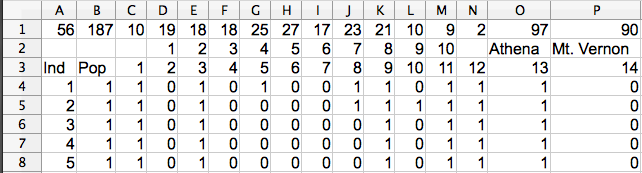
\includegraphics{rootrot2}
\end{figure}
\setkeys{Gin}{width=0.5\textwidth}

% We can reverse it by simply changing the method.
\begin{center}
   \fcolorbox{black}{light-gray}{
         \begin{minipage}[t]{0.8\textwidth}
{\large \textsc{The amazing disappearing options!}}\\
Notice that I'm not writing in many of the options? This is because they have defaults. Since the data frame in my \texttt{@other} slot is called ``population hierarchy", I don't have to specify that every time I do the function call, and that saves a lot of typing! 
% Also, since the hierarchy has already been split into its components, I can now index the data frame by column number. So, since I want to combine the ``Pop" and ``Subpop" components, I will tell the function to use columns 2 through 3.
        \end{minipage}
      }
\end{center}

We'll import our data using \texttt{read.genalex} and take a look at the population hierarchy.
\begin{Schunk}
\begin{Sinput}
> Aeut2 <- read.genalex(system.file("files/rootrot2.csv", package="poppr"), region=TRUE)
> head(Aeut2@other$population_hierarchy)
\end{Sinput}
\begin{Soutput}
  Pop Region
1   1 Athena
2   1 Athena
3   1 Athena
4   1 Athena
5   1 Athena
6   1 Athena
\end{Soutput}
\begin{Sinput}
> summary(Aeut2)
\end{Sinput}
\begin{Soutput}
 # Total number of genotypes:  187 

 # Population sample sizes:  
 1  2  3  4  5  6  7  8  9 10 
19 18 18 25 27 17 23 21 10  9 

 # Percentage of missing data:  
[1] 0
\end{Soutput}
\end{Schunk}
What we see is that we have both of the population factors, but the names have changed and they are not combined. Note that since we specified ``Athena" and ``Mt. Vernon" as regions, the other level of the hierarchy was set as the population factor. We'll use \texttt{splitcombine} to combine both of these in the proper order. Note that we can use the indexes of the data frame columns to index these.

\begin{Schunk}
\begin{Sinput}
> Aeut2.combine <- splitcombine(Aeut2, method=2, hier=2:1)
> head(Aeut2.combine@other$population_hierarchy)
\end{Sinput}
\begin{Soutput}
  Pop Region Region_Pop
1   1 Athena   Athena_1
2   1 Athena   Athena_1
3   1 Athena   Athena_1
4   1 Athena   Athena_1
5   1 Athena   Athena_1
6   1 Athena   Athena_1
\end{Soutput}
\begin{Sinput}
> summary(Aeut2.combine)
\end{Sinput}
\begin{Soutput}
 # Total number of genotypes:  187 

 # Population sample sizes:  
    Athena_1     Athena_2     Athena_3     Athena_4     Athena_5     Athena_6 
           9           12           10           13           10            5 
    Athena_7     Athena_8     Athena_9    Athena_10 Mt. Vernon_1 Mt. Vernon_2 
          11            8           10            9           10            6 
Mt. Vernon_3 Mt. Vernon_4 Mt. Vernon_5 Mt. Vernon_6 Mt. Vernon_7 Mt. Vernon_8 
           8           12           17           12           12           13 

 # Percentage of missing data:  
[1] 0
\end{Soutput}
\end{Schunk}
% <<splitcombine_combine>>=
% Aeut.combine <- splitcombine(Aeut.pop, method=2, hier=2:3)
% head(Aeut.combine$other$population_hierarchy)
% summary(Aeut.combine)
% @
% 
% Let's imagine for a second that these ``hierarchies" are not actually hierarchical, but rather they represent independent variables (For example: the ``Subpop" factor could represent months of the year). In this case, we would want to only analyze the ``Subpop" factor. We can do this by using \texttt{splitcombine} with only one hierarchical level.
% <<splitcombine_subpop>>=
% Aeut.subpop <- splitcombine(Aeut.pop, method=2, hier="Subpop")
% summary(Aeut.subpop)
% poppr(Aeut.subpop, quiet=TRUE)
% @
Having these hierarchies in your data set is important when it comes to clone-censoring your data set (see section \ref{data.manip:cc} \textit{Attack of the Clone Correction}).
%%%%%%%%%%%%%%%%%%%%%%%%%%%%%%%%%%%%%%%%%%%%%%%%%%%%%%%%%%%%%%%%%%%%%%%%%%%%%%%%
%%%%%%%%%%%%%%%%%%%%%%%%%%%%%%%%%%%%%%%%%%%%%%%%%%%%%%%%%%%%%%%%%%%%%%%%%%%%%%%%
%%%%%%%%%%%%%%%%%%%%%%%%%%%%%%%%%%%%%%%%%%%%%%%%%%%%%%%%%%%%%%%%%%%%%%%%%%%%%%%%
\subsection{Divide (populations) and conquer (your analysis) \{extract populations\}}\label{data.manip:divide}

\tab\tab As I've mentioned before, \textit{adegenet} has many ways of sub-setting the data, but you cannot easily subset a \texttt{genind} object by population in an efficient way. \textit{Poppr} allows sub-setting a population from a \texttt{genind} object with one command.
\subsubsection{Function: popsub}\label{data.manip:divide:popsub}

\tab\tab The command \texttt{popsub} is powerful in that it allows you to choose exactly what populations you choose to include or exclude from your analyses. As with many R functions, you can easily use this within a function to avoid creating a new variable to keep track of.  
\begin{quote}
Default Command:\\
\texttt{popsub(pop, sublist = "ALL", blacklist = NULL, mat = NULL)}
\end{quote}
\begin{itemize}
  \item \texttt{pop -} a \texttt{genind} object.
  \item \texttt{sublist -} The vector of populations or integers representing the populations in your data set you wish to retain. For example: \texttt{sublist = c("pop\_z", "pop\_y")} or \texttt{sublist = 1:2}.
  \item \texttt{blacklist -} The vector of populations or integers representing the populations in your data set you wish to exclude. This can take the same type of arguments as sublist, and can be used in conjunction with sublist for when you want a range of populations, but know that there is one in there that you do not want to analyze. For example: \texttt{sublist = 1:15, blacklist = "pop\_x"}.
  One very useful thing about the blacklist is that it allows the user to be extremely paranoid about the data. You can set the blacklist to contain populations that are not even in your data set and it will still work!
  \item \texttt{mat -} (see section \ref{mlg}, \textit{Multilocus Genotype Analysis} for more information) This is where you would put a matrix that's produced by \texttt{mlg.table} to be subsetted instead of the genind object. If you do this, the matrix will return with only the rows equal to your populations and only the multilocus genotypes (columns) pertaining to those populations. 
\end{itemize}

To demonstrate this tool, let's revisit the H3N2 data set. Let's say we wanted to analyze only the data in North America. To make sure we are all on the same page, we will reset the population factor to ``country". Remember that this is located in a data frame in the \texttt{@other} slot called ``x".
\begin{Schunk}
\begin{Sinput}
> data(H3N2)
> pop(H3N2) <- H3N2$other$x$country
> H3N2$pop.names # Only two countries from North America.
\end{Sinput}
\begin{Soutput}
 [1] "Japan"          "USA"            "Finland"        "China"          "South Korea"   
 [6] "Norway"         "Taiwan"         "France"         "Latvia"         "Netherlands"   
[11] "Bulgaria"       "Turkey"         "United Kingdom" "Denmark"        "Austria"       
[16] "Canada"         "Italy"          "Russia"         "Bangladesh"     "Egypt"         
[21] "Germany"        "Romania"        "Ukraine"        "Czech Republic" "Greece"        
[26] "Iceland"        "Ireland"        "Sweden"         "Nepal"          "Saudi Arabia"  
[31] "Switzerland"    "Iran"           "Mongolia"       "Spain"          "Slovenia"      
[36] "Croatia"        "Algeria"       
\end{Soutput}
\begin{Sinput}
> H.na <- popsub(H3N2, sublist=c("USA", "Canada"))
> H.na$pop.names
\end{Sinput}
\begin{Soutput}
      P1       P2 
   "USA" "Canada" 
\end{Soutput}
\end{Schunk}
Since this is a larger data set, running the \texttt{summary} function might take a few seconds longer than we want it to. If we want to see the population size, we can use the \textit{adegenet} function \texttt{nInd()}:
\begin{Schunk}
\begin{Sinput}
> nInd(H.na)
\end{Sinput}
\begin{Soutput}
[1] 665
\end{Soutput}
\begin{Sinput}
> nInd(H3N2)
\end{Sinput}
\begin{Soutput}
[1] 1903
\end{Soutput}
\end{Schunk}
You can see that the population factors are correct and that the size of the data set is considerably smaller. Let's see the data set without the North American countries.
\begin{Schunk}
\begin{Sinput}
> H.minus.na <- popsub(H3N2, blacklist=c("USA", "Canada"))
> H.minus.na$pop.names
\end{Sinput}
\begin{Soutput}
             P01              P02              P03              P04              P05 
         "Japan"        "Finland"          "China"    "South Korea"         "Norway" 
             P06              P07              P08              P09              P10 
        "Taiwan"         "France"         "Latvia"    "Netherlands"       "Bulgaria" 
             P11              P12              P13              P14              P15 
        "Turkey" "United Kingdom"        "Denmark"        "Austria"          "Italy" 
             P16              P17              P18              P19              P20 
        "Russia"     "Bangladesh"          "Egypt"        "Germany"        "Romania" 
             P21              P22              P23              P24              P25 
       "Ukraine" "Czech Republic"         "Greece"        "Iceland"        "Ireland" 
             P26              P27              P28              P29              P30 
        "Sweden"          "Nepal"   "Saudi Arabia"    "Switzerland"           "Iran" 
             P31              P32              P33              P34              P35 
      "Mongolia"          "Spain"       "Slovenia"        "Croatia"        "Algeria" 
\end{Soutput}
\end{Schunk}
Let's make sure that the number of individuals in both data sets added up equals the number of individuals in our original data set:
\begin{Schunk}
\begin{Sinput}
> (nInd(H.minus.na) + nInd(H.na)) == nInd(H3N2)
\end{Sinput}
\begin{Soutput}
[1] TRUE
\end{Soutput}
\end{Schunk}

Now we have data sets with and without North America. Let's try something a bit more challenging. Let's say that we want The first 10 populations in alphabetical order, but we know that we still don't want any countries in North America. We can easily do this by using the \textit{base} function \texttt{sort}.
\begin{Schunk}
\begin{Sinput}
> Hsort <- sort(H3N2$pop.names)[1:10]
> Hsort
\end{Sinput}
\begin{Soutput}
 [1] "Algeria"        "Austria"        "Bangladesh"     "Bulgaria"       "Canada"        
 [6] "China"          "Croatia"        "Czech Republic" "Denmark"        "Egypt"         
\end{Soutput}
\begin{Sinput}
> H.alph <- popsub(H3N2, sublist=Hsort, blacklist=c("USA", "Canada"))
> H.alph$pop.names
\end{Sinput}
\begin{Soutput}
              P1               P2               P3               P4               P5 
         "China"       "Bulgaria"        "Denmark"        "Austria"     "Bangladesh" 
              P6               P7               P8               P9 
         "Egypt" "Czech Republic"        "Croatia"        "Algeria" 
\end{Soutput}
\end{Schunk}
And that, is how you subset your data with poppr!
%%%%%%%%%%%%%%%%%%%%%%%%%%%%%%%%%%%%%%%%%%%%%%%%%%%%%%%%%%%%%%%%%%%%%%%%%%%%%%%%
%%%%%%%%%%%%%%%%%%%%%%%%%%%%%%%%%%%%%%%%%%%%%%%%%%%%%%%%%%%%%%%%%%%%%%%%%%%%%%%%
%%%%%%%%%%%%%%%%%%%%%%%%%%%%%%%%%%%%%%%%%%%%%%%%%%%%%%%%%%%%%%%%%%%%%%%%%%%%%%%%
\subsection{Attack of the clone correction \{clone-censor data sets\}}\label{data.manip:cc}

\tab\tab Clone correction refers to the ability of keeping one observation per clone in a given population (or sub-population). Clone correcting can be hazardous if its done by hand (even on small data sets) and it requires a defined population hierarchy to get relevant results. \textit{Poppr} has a clone correcting function that is able to correct at the lowest level of any defined population hierarchy. Note that clone correction in \textit{poppr} is sensitive to missing data, as it treats all missing data as a single extra allele.
\subsubsection{Function: clonecorrect}\label{data.manip:cc:clonecorrect}

\tab\tab This function will return a clone corrected data set corrected for the lowest population level. Population levels are specified with the \texttt{hier} flag. You can choose to combine the population hierarchy to analyze at the lowest population level by choosing \texttt{combine = TRUE}.
\begin{quote}
Default Command:\\
\texttt{clonecorrect(pop, hier = c(1), dfname = "population\_hierarchy", combine = FALSE, keep = 1)}
\end{quote}
\begin{itemize}
  \item \texttt{pop -} a \texttt{genind} object that has a population hierarchy data frame in the \texttt{@other} slot. Note, the \texttt{genind} object does not necessarily require a population factor to begin with. 
  \item \texttt{hier -} This can be a vector of words or numbers referring to specific column names in your data frame in the \texttt{@other} slot.
  \item \texttt{dfname -} The name of a data frame you have in the \texttt{@other} slot with the population factors.
  \item \texttt{combine -} Do you want to combine the population hierarchy? If it's set to \texttt{FALSE} (default), you will be returned a genind object with the top most hierarchical level as a population factor. 
  \item \texttt{keep -} This flag is to be used if you set \texttt{combine = FALSE}. This will tell clone correct to return a specific combination of your hierarchy. For example, imagine a hierarchy that needs to be clone corrected at three levels: \textit{Population} by \textit{Year} by \textit{Month}. If you wanted to only run an analysis on the \textit{Population} level, you would set \texttt{keep = 1} since \textit{Population} is the first level of the hierarchy. On the other hand, if you wanted to run analysis on \textit{Year} by \textit{Month}, you would set \texttt{keep = 2:3} since those are the second and third levels of the hierarchy. 
\end{itemize}

Let's look at ways to clone-correct our data. We'll look at our \textit{A. euteichies} data since that data set is known to include clonal populations \cite{Grunwald:2006}. Notice that I am not including the options \texttt{dfname} and \texttt{combine} because the default arguments suit my needs.
\begin{Schunk}
\begin{Sinput}
> data(Aeut)
> A.cc <- clonecorrect(Aeut,  hier=c("Pop", "Subpop"), keep=1)
> poppr(A.cc, quiet=TRUE)
\end{Sinput}
\begin{Soutput}
         Pop   N MLG   eMLG    SE     H      G  Hexp   E.5     Ia rbarD        File
1     Athena  76  70 60.621 1.017 4.221 65.636 0.998 0.963  2.535 0.062 rootrot.csv
2 Mt. Vernon  65  50 50.000 0.000 3.796 36.739 0.988 0.821 14.310 0.298 rootrot.csv
3      Total 141 119 59.629 1.854 4.705 96.980 0.997 0.876 13.802 0.260 rootrot.csv
\end{Soutput}
\end{Schunk}
Now let's compare the clone corrected analysis to the uncorrected data set:
\begin{Schunk}
\begin{Sinput}
> poppr(Aeut, quiet=TRUE)
\end{Sinput}
\begin{Soutput}
         Pop   N MLG   eMLG    SE     H      G  Hexp   E.5     Ia rbarD        File
1     Athena  97  70 65.981 1.246 4.063 42.193 0.986 0.721  2.906 0.072 rootrot.csv
2 Mt. Vernon  90  50 50.000 0.000 3.668 28.723 0.976 0.726 13.302 0.282 rootrot.csv
3      Total 187 119 68.453 2.989 4.558 68.972 0.991 0.720 14.371 0.271 rootrot.csv
\end{Soutput}
\end{Schunk}

As you can see from the summary tables, everything all sub-populations have been clone censored to the sub population level with respect to the population hierarchy. Notice how the observed number of individuals \texttt{(N)} decreases in the clone corrected data set.

\subsection{Every day I'm shuffling (data sets)  \{permutations and bootstrap resampling\}}\label{data.manip:shuffle}

\tab\tab A common null hypothesis for populations with mixed reproductive modes is panmixia, or to put it simply: lots of sex. A handy way to test for that is permutation analysis to assess random linkage among loci whereupon you randomly shuffle your data. \textit{Poppr} uses randomly shuffled data sets in order to calculate P-values for the index of association ($I_A$ and $\bar r_d$) \cite{Agapow:2001}. Since there might be other tests where a permutation analysis would be pertinent, a shuffler for \texttt{genind} objects was created with four shuffling schemes: two schemes shuffling without replacement and two shuffling with replacement. Details below.
\subsubsection{Function: shufflepop}\label{data.manip:shuffle:shufflepop}
\begin{quote}
Default Command:\\
\texttt{shufflepop(pop, method = 1)}
\end{quote}
\begin{itemize}
  \item \texttt{pop -} a \texttt{genind} object.
  \item \texttt{method -} a number indicating the method of sampling you wish to use. 
  The following methods are available for use:
  \begin{enumerate}
    \item \textbf{Multilocus permutation} This is called Multilocus permutation because it does the same thing as the permutation analysis in the program \textit{multilocus} by Paul Agapow and Austin Burt \cite{Agapow:2001}. This will shuffle the genotypes at each locus. For example, a single diploid locus with four alleles (1, 2, 3, 4) with the frequencies of 0.1, 0.2, 0.3, and 0.4, respectively:
\begin{Schunk}
\begin{Soutput}
     [,1] [,2]
[1,]    4    4
[2,]    4    1
[3,]    4    3
[4,]    2    2
[5,]    3    3
\end{Soutput}
\end{Schunk}
might become:
\begin{Schunk}
\begin{Soutput}
     [,1] [,2]
[1,]    3    3
[2,]    4    1
[3,]    2    2
[4,]    4    4
[5,]    4    3
\end{Soutput}
\end{Schunk}

Note that you have the same genotypes after shuffling, so at each locus, you will maintain the same allelic frequencies and heterozygosity. So, in this sample, you will only see a homozygote with allele 2. This also ensures that the P-values associated with $I_A$ and $\bar r_d$ are exactly the same (for an explanation, see the end of section \ref{index:iard:ia} of this manual). Unfortunately, if you are trying to simulate a sexual population, this does not make much biological sense as it assumes that alleles are not independently assorting within individuals.
    \item \textbf{Permute Alleles} This is a sampling scheme that will permute alleles within the locus. So, using our example above, our resampling might become:
\begin{Schunk}
\begin{Soutput}
     [,1] [,2]
[1,]    3    2
[2,]    2    4
[3,]    1    3
[4,]    4    3
[5,]    4    4
\end{Soutput}
\end{Schunk}
As you can see, The heterozygosity has changed, yet the allelic frequencies remain the same. Overall this would show you, for example, what would happen if the sample you had underwent panmixis within this sample itself. 
    \item \textbf{Parametric Bootstrap} The previous two schemes reshuffled the observed sample, but the parametric bootstrap uses the allelic frequencies as estimates of what the true allelic frequencies are and uses those as probabilities for each allele when resampling the data with replacement. Here are two samples to show you what I mean.
\begin{Schunk}
\begin{Soutput}
First Sample
\end{Soutput}
\begin{Soutput}
     [,1] [,2]
[1,]    1    3
[2,]    3    3
[3,]    3    2
[4,]    4    4
[5,]    4    2
\end{Soutput}
\begin{Soutput}
Second Sample
\end{Soutput}
\begin{Soutput}
     [,1] [,2]
[1,]    3    4
[2,]    2    3
[3,]    4    2
[4,]    4    4
[5,]    4    2
\end{Soutput}
\end{Schunk}

Notice how the heterozygosity has changed along with the allelic frequencies. The frequencies for alleles 3 and 4 have switched in the first data set, and we've lost allele 1 in the second data set purely by chance! This type of sampling scheme attempts to show you what the true population would look like if it were panmictic and your original sample gave you a basis for estimating expected allele frequencies. Since estimates are made from the observed allele frequencies, small samples will produce skewed results.
    \item \textbf{Non-Parametric Bootstrap} The final method is sampling with replacement, but with no assumption about the distribution of the alleles. 
\begin{Schunk}
\begin{Soutput}
     [,1] [,2]
[1,]    1    3
[2,]    3    3
[3,]    3    1
[4,]    2    2
[5,]    3    1
\end{Soutput}
\end{Schunk}
Again, heterozygosity and allele frequencies are not maintained, but now all of the alleles have a 1 in 4 chance of being chosen.
  \end{enumerate}
\end{itemize}
These shuffling schemes have been implemented for the index of association, but there may be other summary statistics you can use \texttt{shufflepop} for. All you have to do is use the function \texttt{replicate}. Let's use $I_A$ as an example:
\begin{Schunk}
\begin{Sinput}
> data(nancycats)
> nan1 <- popsub(nancycats, 1)
> ia(nan1)
\end{Sinput}
\begin{Soutput}
        Ia      rbarD 
0.16564272 0.02105965 
\end{Soutput}
\begin{Sinput}
> replicate(10, ia(shufflepop(nan1, method = 3), quiet=TRUE))
\end{Sinput}
\begin{Soutput}
             [,1]        [,2]        [,3]        [,4]        [,5]        [,6]       [,7]
Ia    0.015572859 0.078727506 -0.10168980 -0.30046022 -0.26021576 -0.25668449 0.25675321
rbarD 0.001964457 0.009966246 -0.01284299 -0.03823542 -0.03314723 -0.03298552 0.03244442
             [,8]        [,9]        [,10]
Ia    -0.28757799 -0.10313192 -0.071845794
rbarD -0.03681791 -0.01306466 -0.009271283
\end{Soutput}
\end{Schunk}
You could use this method to replicate the resampling 999 times and then create a histogram to visualize a distribution of what would happen under different assumptions of panmixia.

\subsection{Cut It Out!  \{removing uninformative loci\}}\label{data.manip:informloci}
 \tab\tab Phylogenetically uninformative loci are those that have only one sample differentiating from the rest. This can lead to biased results when using multilocus analyses such as the index of association (See \ref{index:iard} and \ref{summary}). These nuisance loci can be removed with the following function.
\subsubsection{Function: informloci}\label{data.manip:informloci:informloci}
\begin{quote}
Default Command:\\
\texttt{informloci(pop, cutoff = 2/nInd(pop), quiet = FALSE)}
\end{quote}
  \begin{itemize}
    \item \texttt{pop -} a \texttt{genind} object.
    \item \texttt{cutoff -} this represents the minimum fraction of individuals needed for a locus to be considered informative. The default is set to $2/n$ with $n$ being the number of individuals in the data set (represented by the \textit{adegenet} function \texttt{nInd}). Essentially, this means that any locus with fewer than 2 observations differing will be removed. The user can also specify a fraction of observations for the cutoff (eg. 0.05).
    \item \texttt{quiet -} if \texttt{TRUE}, nothing will be printed to the screen, if \texttt{FALSE}, the cutoff value in percentage and number of individuals will be printed as well as the names of the uninfomrative loci found. 
  \end{itemize}

Here's a quick example.
\begin{Schunk}
\begin{Sinput}
> data(H3N2)
> H.five <- informloci(H3N2, cutoff = 0.05)
\end{Sinput}
\end{Schunk}
\begin{Schunk}
\begin{Soutput}
cutoff value: 5 percent ( 95 individuals ).
 47 uninfomative loci found: 157 
177 233 243 262 267 280 303 313 327 357 382 384 399 412 418 424 425 429 433 451 
470 529 546 555 557 564 576 592 595 597 602 612 627 642 647 648 654 658 663 667 
681 717 806 824 837 882
\end{Soutput}
\end{Schunk}
Now what happens when you have all informative loci:
\begin{Schunk}
\begin{Sinput}
> data(nancycats)
> naninform <- informloci(nancycats, cutoff = 0.05)
\end{Sinput}
\begin{Soutput}
cutoff value: 5 percent ( 12 individuals ).
No sites found with fewer than 12 different individuals.
\end{Soutput}
\end{Schunk}

%%%%%%%%%%%%%%%%%%%%%%%%%%%%%%%%%%%%%%%%%%%%%%%%%%%%%%%%%%%%%%%%%%%%%%%%%%%%%%%%
%%%%%%%%%%%%%%%%%%%%%%%%%%%%%%%%%%%%%%%%%%%%%%%%%%%%%%%%%%%%%%%%%%%%%%%%%%%%%%%%
%%%%%%%%%%%%%%%%%%%%%%%%%%%%%%%%%%%%%%%%%%%%%%%%%%%%%%%%%%%%%%%%%%%%%%%%%%%%%%%%
\section{Multilocus Genotype Analysis}\label{mlg}

\tab\tab In populations with mixed sexual and clonal reproduction, it is not uncommon to have multiple samples from the same population have the same genotype across multiple loci (multilocus genotype, MLG). Here, we introduce tools for tracking MLGs within and across populations in \texttt{genind} objects from the \textit{adegenet} package. We will be using SNP data from isolates of the H3N2 virus from 2002 to 2006.
\subsection{Just a peek \{How many multilocus genotypes are in our data set?\}}\label{mlg:mlg}

\tab\tab First, let's take a quick look at how many Multilocus Genotypes are present within the H3N2 data set using the \texttt{mlg} function. This will tell us if any MLG analysis is needed.
\subsubsection{Function: mlg}\label{mlg:mlg:mlg}

\tab\tab The function \texttt{mlg} allows for the counting of the number of MLGs in a \texttt{genind} object. This is a very simple command for quick reference to determine if your data set needs further multilocus genotype analysis.
\begin{quote}
Default Command:\\
\texttt{mlg(pop, quiet = FALSE)}
\end{quote}
  \begin{itemize}
    \item \texttt{pop -} a \texttt{genind} object.
    \item \texttt{quiet -} if \texttt{TRUE}, the number of individuals and multilocus genotypes will be printed to the screen, if \texttt{FALSE}, nothing will be printed to the screen and the number of multilocus genotypes will be reported.
  \end{itemize}
\begin{Schunk}
\begin{Sinput}
> data(H3N2)
> mlg(H3N2, quiet=FALSE)
\end{Sinput}
\begin{Soutput}
#############################
# Number of Individuals: 1903 
# Number of MLG: 752 
#############################
[1] 752
\end{Soutput}
\end{Schunk}
We can see that since the number of individuals exceeds the number of multilocus genotypes, this data set contains clones. Let's take a look at where those clones are with respect to populations.
\subsection{Clone-ing around \{MLGs across populations\}}\label{mlg:cross}

\tab\tab Since you have the ability to change the population structure of your data set freely, it is quite possible to see some of the same MLGs across different populations. Tracking them by hand can be a nightmare with large data sets. Luckily, \texttt{mlg.crosspop} has you covered in that regard.
\subsubsection{Function: mlg.crosspop}\label{mlg:cross:mlg.crosspop}

\tab\tab Analyze the MLGs that cross populations within your data set. This has three output modes. The default one gives a list of MLGs, and for each MLG, it gives a named numeric vector indicating the abundance of that MLG in each population. Alternate outputs are described with \texttt{indexreturn} and \texttt{df}.
\begin{quote}
Default Command:\\
\texttt{mlg.crosspop(pop, sublist = "ALL", blacklist = NULL, mlgsub = NULL, indexreturn = FALSE, df = FALSE, quiet = FALSE)}
\end{quote}
  \begin{itemize}
    \item \texttt{pop -} a \texttt{genind} object.
    \item \texttt{sublist -} see \texttt{mlg.table}, Section \ref{mlg:table:mlg.table}. Analyze specified populations.
    \item \texttt{blacklist -} see \texttt{mlg.table}, Section \ref{mlg:table:mlg.table}. Do not include specified populations.
    \item \texttt{mlgsub -} see \texttt{mlg.table}, Section \ref{mlg:table:mlg.table}. Only analyze specified MLGs. The vector for this flag can be produced by this function as you will see later in this vignette.
    \item \texttt{indexreturn -} return a vector of indices of MLGs. (You can use these in the \texttt{mlgsub} flag, or you can use them to subset the columns of an MLG table). 
    \item \texttt{df -} return a data frame containing the MLGs, the populations they cross, and the number of copies you find in each population. This is useful for making graphs in \textit{ggplot2}.
    \item \texttt{quiet -} \texttt{TRUE} or \texttt{FALSE}. Should the populations be printed to screen as they are processed? (will print nothing if \texttt{indexreturn} is \texttt{TRUE})
  \end{itemize}
  
We can see what Multilocus Genotypes cross different populations and then give a vector that shows how many populations each multi-population MLG crosses.
\begin{Schunk}
\begin{Sinput}
> pop(H3N2) <- H3N2$other$x$country
> H.dup <- mlg.crosspop(H3N2, quiet=TRUE)
\end{Sinput}
\end{Schunk}
Here is a snippet of what the output looks like when \texttt{quiet} is \texttt{FALSE}. It will print out the MLG name, the total number of individuals that make up that MLG, and the populations where that MLG can be found.
\begin{Schunk}
\begin{Soutput}
MLG.3: (12 inds) USA Denmark
MLG.9: (16 inds) Japan USA Finland Denmark
MLG.31: (9 inds) Japan Canada
MLG.75: (23 inds) Japan USA Finland Norway Denmark Austria Russia Ireland
MLG.80: (2 inds) USA Denmark
MLG.86: (7 inds) Denmark Austria
MLG.95: (2 inds) USA Bangladesh
MLG.97: (8 inds) USA Austria Bangladesh Romania
MLG.104: (3 inds) USA France
MLG.110: (16 inds) Japan USA China
\end{Soutput}
\end{Schunk}
The output of this function is a list of MLGs, each containing a vector indicating the number of copies in each population. We'll count the number of populations each MLG crosses using the function \texttt{sapply} with \texttt{length}.
\begin{Schunk}
\begin{Sinput}
> head(H.dup)
\end{Sinput}
\begin{Soutput}
$MLG.3
    USA Denmark 
      4       8 

$MLG.9
  Japan     USA Finland Denmark 
      1      13       1       1 

$MLG.31
 Japan Canada 
     2      7 

$MLG.75
  Japan     USA Finland  Norway Denmark Austria  Russia Ireland 
      2       8       2       1       6       2       1       1 

$MLG.80
    USA Denmark 
      1       1 

$MLG.86
Denmark Austria 
      3       4 
\end{Soutput}
\begin{Sinput}
> H.num <- sapply(H.dup, length) # count the number of populations each MLG crosses.
> H.num
\end{Sinput}
\begin{Soutput}
  MLG.3   MLG.9  MLG.31  MLG.75  MLG.80  MLG.86  MLG.95  MLG.97 MLG.104 MLG.110 MLG.119 
      2       4       2       8       2       2       2       4       2       3       2 
MLG.149 MLG.158 MLG.163 MLG.205 MLG.206 MLG.207 MLG.210 MLG.213 MLG.221 MLG.224 MLG.227 
      2       6       2       2       3       2       2       4       2       3       3 
MLG.234 MLG.241 MLG.244 MLG.246 MLG.252 MLG.253 MLG.258 MLG.274 MLG.277 MLG.283 MLG.285 
      6       3       2      10       2       9       2       5       3       3       2 
MLG.290 MLG.291 MLG.314 MLG.315 MLG.317 MLG.321 MLG.325 MLG.326 MLG.334 MLG.344 MLG.350 
      3       2       2       3       3       2       2       2       2       2       2 
MLG.368 MLG.370 MLG.381 MLG.401 MLG.405 MLG.417 MLG.439 MLG.453 MLG.461 MLG.471 MLG.508 
      3       2       3       3       3       5       2       2       3       2       3 
MLG.529 MLG.530 MLG.540 MLG.548 MLG.552 MLG.556 MLG.570 MLG.578 MLG.580 MLG.582 MLG.589 
      5       3       3       2       2       2       2       2       2       2       2 
MLG.597 MLG.605 MLG.611 MLG.615 MLG.619 MLG.620 MLG.621 
      2       3       2       2       2       4       2 
\end{Soutput}
\end{Schunk}
%\newpage
\subsection{Bringing something to the table \{producing MLG tables and graphs\}}\label{mlg:table}

We can also create a table of multilocus genotypes per population as well as bar graphs to give us a visual representation of the data. This is achieved through the function \texttt{mlg.table}
\subsubsection{Function: mlg.table}\label{mlg:table:mlg.table}

\tab\tab Produce a matrix containing counts of MLGs (columns) per population (rows). If there is no population structure to your data set, a vector will be produced instead.
\begin{quote}
Default Command:\\
\texttt{mlg.table(pop, sublist = "ALL", blacklist = NULL, mlgsub = NULL, bar = TRUE, total = FALSE, quiet = FALSE)}
\end{quote}
  \begin{itemize}
    \item \texttt{pop -} a \texttt{genind} object.
    \item \texttt{sublist -} a vector indicating which specific populations you want to produce a table for. This can be a numeric or character vector. See section \ref{data.manip:divide:popsub} for details.
    \item \texttt{blacklist -} a vector indicating which specific populations you do not want to include in your table. This can be a numeric or character vector, and does not necessarily have to be the same type as \texttt{sublist}. eg. \texttt{sublist=1:10, blacklist="USA"}. See section \ref{data.manip:divide:popsub} for details.
    \item \texttt{mlgsub -} a vector containing the indices of MLGs you wish to subset your table with. 
    \item \texttt{bar -} \texttt{TRUE} or \texttt{FALSE}. If  \texttt{TRUE}, a bar plot will be printed for each population with more than one individual. 
    \item \texttt{total -} \texttt{TRUE} or \texttt{FALSE}. Should the entire data set be included in the table? This is equivalent to evoking \texttt{colSums} on the table.
    \item \texttt{quiet -} \texttt{TRUE} or \texttt{FALSE}. When \texttt{bar} is \texttt{TRUE}, should the populations be printed to screen as they are processed?
  \end{itemize}
\begin{Schunk}
\begin{Sinput}
> H.tab <- mlg.table(H3N2, quiet=TRUE, bar=TRUE)
> H.tab[1:10, 1:10] # Showing the first 10 columns and rows of the table.
\end{Sinput}
\end{Schunk}
\begin{Schunk}
\begin{Soutput}
            MLG.1 MLG.2 MLG.3 MLG.4 MLG.5 MLG.6 MLG.7 MLG.8 MLG.9 MLG.10
Japan           0     0     0     0     0     0     1     2     1      0
USA             0     2     4     1     1     0     0     0    13      0
Finland         0     0     0     0     0     0     0     0     1      0
China           0     0     0     0     0     0     0     0     0      0
South Korea     0     0     0     0     0     1     0     0     0      0
Norway          1     0     0     0     0     0     0     0     0      0
Taiwan          0     0     0     0     0     0     0     0     0      0
France          0     0     0     0     0     0     0     0     0      0
Latvia          0     0     0     0     0     0     0     0     0      0
Netherlands     0     0     0     0     0     0     0     0     0      0
\end{Soutput}
\end{Schunk}
\begin{figure}[h!]
  \centering
  \caption{\footnotesize An example of a bar-chart produced by \texttt{mlg.table}. Note that this data set would produce several such charts.}
  \label{nortable}
\includegraphics{poppr_manual-mlgbarplot}
\end{figure}
\newpage

The MLG table is not restricted for use with just \textit{Poppr}. One of the main advantages of the function \texttt{mlg.table} is that it allows easy access to diversity functions present in the package \textit{vegan} \cite{vegan}. One very simple example is to create a rarefaction curve for each population in your data set giving the number of expected MLGs for a given sample size. For more information, type \texttt{help("diversity", package="vegan")} in your R console.

For the sake of a simple example, instead of drawing a curve for each of the 37 countries represented in this sample, let's change the population structure to be the different years of the epidemics. 
\begin{Schunk}
\begin{Sinput}
> H.year <- H3N2
> pop(H.year) <- H.year$other$x$year
> summary(H.year) # Check the data to make sure it's correct.
\end{Sinput}
\begin{Soutput}
 # Total number of genotypes:  1903 

 # Population sample sizes:  
2002 2003 2004 2005 2006 
 158  415  399  469  462 

 # Number of alleles per locus:  
L001 L002 L003 L004 L005 L006 L007 L008 L009 L010 L011 L012 L013 L014 L015 L016 L017 L018 
   3    3    4    2    4    2    3    2    4    3    4    2    4    3    2    2    3    3 
L019 L020 L021 L022 L023 L024 L025 L026 L027 L028 L029 L030 L031 L032 L033 L034 L035 L036 
   2    2    3    3    3    2    2    2    2    2    2    2    2    2    2    4    4    3 
L037 L038 L039 L040 L041 L042 L043 L044 L045 L046 L047 L048 L049 L050 L051 L052 L053 L054 
   3    3    4    2    2    2    4    3    2    3    4    2    3    2    3    2    2    2 
L055 L056 L057 L058 L059 L060 L061 L062 L063 L064 L065 L066 L067 L068 L069 L070 L071 L072 
   4    2    2    2    2    2    2    2    4    4    4    3    3    2    3    4    3    2 
L073 L074 L075 L076 L077 L078 L079 L080 L081 L082 L083 L084 L085 L086 L087 L088 L089 L090 
   3    3    3    3    2    3    2    4    2    3    2    2    3    3    3    3    2    2 
L091 L092 L093 L094 L095 L096 L097 L098 L099 L100 L101 L102 L103 L104 L105 L106 L107 L108 
   2    2    3    2    3    2    3    2    3    2    3    3    2    2    2    3    2    2 
L109 L110 L111 L112 L113 L114 L115 L116 L117 L118 L119 L120 L121 L122 L123 L124 L125 
   2    3    3    3    2    2    3    3    3    3    4    2    3    3    4    3    2 

 # Number of alleles per population:  
  1   2   3   4   5 
203 255 232 262 240 

 # Percentage of missing data:  
[1] 2.363426

 # Observed heterozygosity:  
[1] 0

 # Expected heterozygosity:  
[1] 0
\end{Soutput}
\end{Schunk}
\begin{Schunk}
\begin{Sinput}
> library(vegan)
> H.year <- mlg.table(H.year, bar=FALSE)
> rarecurve(H.year, ylab="Multilocus genotypes expected", sample=min(rowSums(H.year)))
\end{Sinput}
\end{Schunk}
\begin{figure}[h!]
  \centering
  \caption{\footnotesize An example of a rarefaction curve produced using a MLG table.}
  \label{rarecurve}
\includegraphics{poppr_manual-mlgrareplot}
\end{figure}
\newpage

The minimum value from the \textit{base} function \texttt{rowSums()} of the table represents the minimum common sample size of all populations. Setting the ``sample" flag draws the horizontal and vertical lines you see on the graph. The intersections of these lines correspond to the numbers you would find if you ran the function \texttt{poppr} on this data set (under the column ``\texttt{eMLG}").
%%%%%%%%%%%%%%%%%%%%%%%%%%%%%%%%%%%%%%%%%%%%%%%%%%%%%%%%%%%%%%%%%%%%%%%%%%%%%%%%
%%%%%%%%%%%%%%%%%%%%%%%%%%%%%%%%%%%%%%%%%%%%%%%%%%%%%%%%%%%%%%%%%%%%%%%%%%%%%%%%
\subsection{Getting into the mix \{combining MLG functions\}}\label{mlg:mix}

\tab\tab Alone, the different functionalities are neat. Combined, we can create interesting data sets. Let's say we wanted to know which MLGs were duplicated across the regions of the United Kingdom, Germany, Netherlands, and Norway. All we have to do is use the \texttt{sublist} flag in the function:
\begin{Schunk}
\begin{Sinput}
> UGNN.list <- c("United Kingdom", "Germany", "Netherlands", "Norway")
> UGNN <- mlg.crosspop(H3N2, sublist=UGNN.list, indexreturn=TRUE)
\end{Sinput}
\end{Schunk}
OK, the output tells us that there are three MLGs that are crossing between these
populations, but we do not know how many are in each. We can easily find that out if we subset our original table, \texttt{H.tab}. 

\begin{Schunk}
\begin{Sinput}
> UGNN # Note that we have three numbers here. This will index the columns for us.
\end{Sinput}
\begin{Soutput}
MLG.315 MLG.317 MLG.620 
    315     317     620 
\end{Soutput}
\begin{Sinput}
> UGNN.list # And let's not forget that we have the population names.
\end{Sinput}
\begin{Soutput}
[1] "United Kingdom" "Germany"        "Netherlands"    "Norway"        
\end{Soutput}
\begin{Sinput}
> H.tab[UGNN.list, UGNN]
\end{Sinput}
\begin{Soutput}
               MLG.315 MLG.317 MLG.620
United Kingdom       1       0       0
Germany              0       1       1
Netherlands          0       0       0
Norway               2       3       1
\end{Soutput}
\end{Schunk}

Now we can see that Norway has a higher incidence of nearly all of these MLGs. 
We can go even further and subset the original data set to only give us those MLGs by utilizing the function \texttt{mlg.vector}:
\subsubsection{Function: mlg.vector}\label{mlg:mix:mlg.vector}

\tab\tab This function is the backbone for \texttt{mlg.table} and \texttt{mlg.crosspop}, and is The function that determines what your MLGs are. This is quite useful for sub-setting the data set to only contain the MLGs of interest. The numbers in the vector correspond to the number of columns in a matrix produced by \texttt{mlg.table}. It is important to remember that this is also sensitive to missing data and will treat it as a single extra allele. 
\begin{quote}
Default Command:\\
\texttt{mlg.vector(pop)}
\end{quote}
  \begin{itemize}
    \item \texttt{pop -} a \texttt{genind} object.
  \end{itemize}
\begin{Schunk}
\begin{Sinput}
> H.vec <- mlg.vector(H3N2)
> H.sub <- H3N2[H.vec %in% UGNN, ]
> mlg.table(H.sub, bar=FALSE)
\end{Sinput}
\begin{Soutput}
               MLG.1 MLG.2 MLG.3
Austria            0     0     7
Germany            0     1     1
Greece             0     0     1
Norway             2     3     1
Japan              4     1     0
United Kingdom     1     0     0
\end{Soutput}
\end{Schunk}
You can also do the same thing using the mlgsub flag.
\begin{Schunk}
\begin{Sinput}
> mlg.table(H3N2, mlgsub=UGNN, bar=TRUE)
\end{Sinput}
\end{Schunk}
\begin{Schunk}
\begin{Soutput}
               MLG.315 MLG.317 MLG.620
Japan                4       1       0
Norway               2       3       1
United Kingdom       1       0       0
Austria              0       0       7
Germany              0       1       1
Greece               0       0       1
\end{Soutput}
\end{Schunk}
And we can see where exactly these three MLGs fall within our data set.
\begin{figure}[h!]
  \centering
  \caption{\footnotesize An example of the same bar-chart as \textit{Figure 1}, but focusing on three MLGs.}
  \label{nortable2}
\includegraphics{poppr_manual-subnor}
\end{figure}
\\
\newpage
Now, you might notice that the MLG vector no longer matches up with our data after we subset it.
\begin{Schunk}
\begin{Sinput}
> H.vec[1:22]
\end{Sinput}
\begin{Soutput}
 [1] 605 605 672 675 674 673 670 671 670 678 678 678 678 582 615 580 581 570 615 582 582
[22] 592
\end{Soutput}
\begin{Sinput}
> mlg.vector(H.sub)
\end{Sinput}
\begin{Soutput}
 [1] 3 3 3 3 3 3 3 3 3 3 2 1 1 2 2 1 2 1 1 1 1 2
\end{Soutput}
\end{Schunk}
Well, this is unfortunate because it means that we can't compare any subsetted data with non-subsetted data. Luckily, there's a little trick we can do using our old friend, the \texttt{@other} slot.
If we place the MLG vector in the \texttt{@other} slot of our original data set, it will be subsetted along with the data.
\begin{Schunk}
\begin{Sinput}
> H3N2@other$MLG.vector <- H.vec
> H.sub <- H3N2[H.vec %in% UGNN, ]
> H.sub@other$MLG.vector
\end{Sinput}
\begin{Soutput}
 [1] 620 620 620 620 620 620 620 620 620 620 317 315 315 317 317 315 317 315 315 315 315
[22] 317
\end{Soutput}
\end{Schunk}
Magic!\\
%\newpage

So, we've gotten this far, yet we haven't actually seen what the genotypes look like! For analyses where the genotypic signature is important, this is a crucial identification step. Lucky for us, the \texttt{genind} object retains all of the genotypic information and can be accessed using the \texttt{genind2df} function. Let's take a look at the three genotypes we specified above utilizing the vector of MLGs we created above, \texttt{H.vec}.
\begin{Schunk}
\begin{Sinput}
> H.df <- genind2df(H3N2)
> H.df[H.vec %in% UGNN, 1:15] # Showing only 15 columns becaus it is a large dataset.
\end{Sinput}
\end{Schunk}
\begin{Schunk}
\begin{Soutput}
                    pop 6 17 39 42 45 51 60 72 73 90 108 123 129 134
CY026119        Austria a  a  g  c  g  c  g  g  c  g   a   g   t   g
CY026120        Austria a  a  g  c  g  c  g  g  c  g   a   g   t   g
CY026121        Austria a  a  g  c  g  c  g  g  c  g   a   g   t   g
CY026122        Austria a  a  g  c  g  c  g  g  c  g   a   g   t   g
CY026131        Austria a  a  g  c  g  c  g  g  c  g   a   g   t   g
CY026132        Austria a  a  g  c  g  c  g  g  c  g   a   g   t   g
CY026135        Austria a  a  g  c  g  c  g  g  c  g   a   g   t   g
EU502462        Germany a  a  g  c  g  c  g  g  c  g   a   g   t   g
EU502463         Greece a  a  g  c  g  c  g  g  c  g   a   g   t   g
EU502464         Norway a  a  g  c  g  c  g  g  c  g   a   g   t   g
EU501513          Japan a  a  g  c  t  c  a  g  a  g   t   g   t   g
AB243868          Japan a  a  g  c  t  c  a  g  a  g   t   g   t   g
DQ883618         Norway a  a  g  c  t  c  a  g  a  g   t   g   t   g
DQ883619         Norway a  a  g  c  t  c  a  g  a  g   t   g   t   g
DQ883620         Norway a  a  g  c  t  c  a  g  a  g   t   g   t   g
DQ883628         Norway a  a  g  c  t  c  a  g  a  g   t   g   t   g
EU501609        Germany a  a  g  c  t  c  a  g  a  g   t   g   t   g
EU501642          Japan a  a  g  c  t  c  a  g  a  g   t   g   t   g
EU501643          Japan a  a  g  c  t  c  a  g  a  g   t   g   t   g
EU501735 United Kingdom a  a  g  c  t  c  a  g  a  g   t   g   t   g
EU501742          Japan a  a  g  c  t  c  a  g  a  g   t   g   t   g
EU502513         Norway a  a  g  c  t  c  a  g  a  g   t   g   t   g
\end{Soutput}
\end{Schunk}
Notice that there seems to be a clear separation between the SNPs of the first 10 isolates and the rest? This is no coincidence. Take a look at the output of our sub-setting.
\begin{Schunk}
\begin{Sinput}
> UGNN
\end{Sinput}
\begin{Soutput}
MLG.315 MLG.317 MLG.620 
    315     317     620 
\end{Soutput}
\begin{Sinput}
> H.vec[H.vec %in% UGNN]
\end{Sinput}
\begin{Soutput}
 [1] 620 620 620 620 620 620 620 620 620 620 317 315 315 317 317 315 317 315 315 315 315
[22] 317
\end{Soutput}
\end{Schunk}

We have the MLGs 315, 317, and 620, and the result of the sub-setting shows us that 620 occurs earlier in our data set, and that MLGs 315 and 317 are mixed in together. The reason why we do not see a mixture of three different sets of SNP calls in our little window is because \texttt{mlg.vector} creates the MLGs by first concatenating and then sorting the genotypes. This way, the closer two MLG indexes are to each other, the fewer differences they will have between one another. 
%%%%%%%%%%%%%%%%%%%%%%%%%%%%%%%%%%%%%%%%%%%%%%%%%%%%%%%%%%%%%%%%%%%%%%%%%%%%%%%%
%%%%%%%%%%%%%%%%%%%%%%%%%%%%%%%%%%%%%%%%%%%%%%%%%%%%%%%%%%%%%%%%%%%%%%%%%%%%%%%%
\subsection{Do you see what I see? \{alternative data visualization\}}\label{mlg:alt.vis}

\tab\tab The graphs that are output by \textit{poppr} are simply aids for the user to make data analysis easier. We want to better visualize how these MLGs cross populations by MLG or population. We also want to see exactly what MLGs are in which populations, and how prevalent they are. As the package \textit{ggplot2} is based on data frames, we have to give ourselves a data frame to work with. We can do this using the \texttt{df = TRUE} flag.
\begin{Schunk}
\begin{Sinput}
> df <- mlg.crosspop(H3N2, df=TRUE, quiet=TRUE)
> names(df)
\end{Sinput}
\begin{Soutput}
[1] "MLG"        "Population" "Count"     
\end{Soutput}
\end{Schunk}
Now that we have our data frame, we can do a couple of things. We can first see where the most omnipresent MLG occurs. After that, we will plot the top ten MLGs using ggplot2.
\begin{Schunk}
\begin{Sinput}
> H.max <- names(sort(H.num, decreasing=TRUE)[1:10])
> # Showing the data frame by the largest MLG complex.
> df[df$MLG %in% H.max[1], ]
\end{Sinput}
\begin{Soutput}
       MLG  Population Count
76 MLG.246       Japan     3
77 MLG.246         USA     8
78 MLG.246       China     4
79 MLG.246      Norway     1
80 MLG.246     Austria     6
81 MLG.246      Russia     1
82 MLG.246       Egypt     1
83 MLG.246     Iceland     1
84 MLG.246       Nepal    15
85 MLG.246 Switzerland     1
\end{Soutput}
\end{Schunk}
And now we can visualize the largest ten MLG complexes using \textit{ggplot2}'s \texttt{qplot} function.
\begin{figure}[h]
  \centering
  \caption{\footnotesize An example of the versatility of the MLG information.}
  \label{mlgtable2}
\begin{Schunk}
\begin{Sinput}
> df2 <- df[df$MLG %in% H.max, ]
> library(ggplot2)
> qplot(y=MLG, x=Population, data=df2, color=Count, size=Count) +
+   theme(axis.text.x = element_text(size = 10, angle = -45, hjust = 0))
\end{Sinput}
\end{Schunk}
\includegraphics{poppr_manual-ggplotchart}
\end{figure}
%%%%%%%%%%%%%%%%%%%%%%%%%%%%%%%%%%%%%%%%%%%%%%%%%%%%%%%%%%%%%%%%%%%%%%%%%%%%%%%%
%%%%%%%%%%%%%%%%%%%%%%%%%%%%%%%%%%%%%%%%%%%%%%%%%%%%%%%%%%%%%%%%%%%%%%%%%%%%%%%%
%%%%%%%%%%%%%%%%%%%%%%%%%%%%%%%%%%%%%%%%%%%%%%%%%%%%%%%%%%%%%%%%%%%%%%%%%%%%%%%%
%%%%%%%%%%%%%%%%%%%%%%%%%%%%%%%%%%%%%%%%%%%%%%%%%%%%%%%%%%%%%%%%%%%%%%%%%%%%%%%%
\section{Index and Distance Calculations}\label{index}
\subsection{The missing linkage disequilibrium \{calculating the index of association, $I_A$ and $\bar r_d$\}}\label{index:iard}

\tab\tab The index of association was originally developed as a measure of multilocus linkage disequilibrium \cite{Brown:1980} and was found to be able to detect signatures of sexual reproduction and population structure \cite{Brown:1980, Smith:1993}. Unfotunately, $I_A$ was found to increase with the number of loci, and was not suitable to comparisons across studies \cite{Agapow:2001}. To remedy this, $\bar{r}_d$ was developed that corrects for this scaling and forces the index to lie between 0 (linkage equilibrium) and 1 (full disequilibrium). $I_A$ has previously been implemented in a couple of programs including \textit{multilocus} \cite{Agapow:2001} and \textit{LIAN} \cite{Haubold:2000}. While both of these programs are still available for download, \textit{multilocus} is no longer actively supported, and \textit{LIAN}, despite its speed, is only appropriate for haplotypic data. Both of these programs each require one specific file format, and, until recently\footnote{LIAN 3.6 allows the user to run multiple contiguous data sets within a single file or across multiple files. It is impossible to run MULTILOCUS in batch.}, neither of these programs had an internal ability to run in batch across multiple populations within a file or multiple files within a directory in the same way that poppr can (see footnote).

It is important to note that for this algorithm, all missing values are treated in the same way as \textit{multilocus} in that all missing alleles are imputed to be the same as the alleles they are being compared to. Depending on the percent missing data in your data set, this might influence the statistic. If you have a lot of missing data, consider using the \texttt{missing} flag in this function.
\subsubsection{Function: ia}\label{index:iard:ia}

\tab\tab This function is a quick look at a single data set. It can do almost everything that \texttt{poppr} can do except for sorting through populations.
\begin{quote}
Default Command:\\
\texttt{ia(pop, sample = 0, method = 1, quiet = FALSE, missing = "ignore", 
    hist = TRUE)}
\end{quote}
\begin{itemize}
  \item \texttt{pop -} a \texttt{genind} object.
  \item \texttt{sample -} You should use this flag whenever you want to reshuffle your data set. Indicate how many times you want to reshuffle your data set to obtain a P-value. 
  \item \texttt{method -} a number from 1 to 4 indicating the sampling method:
  \begin{enumerate}
    \item \textit{multilocus} style permutation \cite{Agapow:2001}.
    \item permutation over alleles.
    \item parametric bootstrap.
    \item non-parametric bootstrap.
  \end{enumerate}
  The methods are detailed in section \ref{data.manip:shuffle:shufflepop} of this manual.
  \item \texttt{quiet -} If set to \texttt{TRUE}, nothing will be printed to the screen as the sampling progresses. If \texttt{FALSE} will produce a progress bar.
  \item \texttt{missing -} This will preprocess your missing values. It is set to ignore missing data, so that they do not contribute to the distance measure. It can also be set to \texttt{"loci", "geno", "zero", or "mean"}. For details, see section \ref{data.manip:missing:missingno} of this manual.
  \item \texttt{hist -} This will produce a pair of histograms for each population showing the distribution of $I_A$ and $\bar r_d$ across the sampled data sets, and plot the observed value as a single vertical line.
\end{itemize}
Running the analysis is as simple as this:
\begin{Schunk}
\begin{Sinput}
> ia(nancycats)
\end{Sinput}
\begin{Soutput}
        Ia      rbarD 
0.17207262 0.02178965 
\end{Soutput}
\end{Schunk}
We can use \texttt{popsub} to subset for specific populations. Here, we'll also demonstrate the sampling flag and show you what the histogram looks like.
\begin{Schunk}
\begin{Sinput}
> set.seed(1001)
> ia(popsub(nancycats, 5), sample=999)
\end{Sinput}
\end{Schunk}
\begin{Schunk}
\begin{Soutput}
|================================================================================| 100%
\end{Soutput}
\begin{Soutput}
          Ia         p.Ia        rbarD         p.rD 
-0.047539953  0.589000000 -0.006004254  0.589000000 
\end{Soutput}
\end{Schunk}

This analysis produced the histograms you see below. What these histograms represent are 999 resamplings of the data under the null hypothesis ($H_0$) of sexual reproduction. The way that $H_0$ is created is determined by the sampling method chosen. In this case, the method was to shuffle genotypes at each locus to simulate unlinked loci. Since the P = 0.589, we would fail to reject $H_0$ and we therefore might conclude that this population is sexually reproducing \cite{Brown:1980} \cite{Smith:1993} \cite{Agapow:2001}.
\begin{figure}[h!]
  \centering
  \caption{\footnotesize Histograms of 999 values of $I_A$ and $\bar{r}_d$ calculated from 999 resamplings of population 5 from the data set ``nancycats". The observed values of $I_A$ and $\bar r_d$ are represented as vertical blue lines overlaid on the distributions. The ticks at the bottom of each histogram represent individual observations.}
  \label{ia_demo_fig}
\includegraphics{poppr_manual-109}
\end{figure}
%\newpage

Note that both of the P-values are exactly the same. This is what you would obtain with the default sampling scheme because the variances within loci do not change. When you change the sampling scheme, however, the P-values can end up being different. That's why there are two fields for P-values. Let's look at what happens to the P-values once we change the sampling scheme to a parametric bootstrap.
\begin{Schunk}
\begin{Sinput}
> set.seed(1001)
> ia(popsub(nancycats, 5), sample=999, method=3, quiet=TRUE, hist=FALSE)
\end{Sinput}
\end{Schunk}
\begin{Schunk}
\begin{Soutput}
          Ia         p.Ia        rbarD         p.rD 
-0.047539953  0.589000000 -0.006004254  0.596000000 
\end{Soutput}
\end{Schunk}
There, is, of course one little caveat that needs to be mentioned. The P-values are calculated by comparing how many permuted values are greater than or equal to the observed value. This includes the observed value (which is why setting the randomizations to 999 will give you a round P-value) which means that the lowest P-value you will ever have is $1/(n+1)$ where $n$ is the number of permutations you select. Take for example this population of a clonal root rot pathogen, \textit{Aphanomyces euteiches}:
\begin{Schunk}
\begin{Sinput}
> data(Aeut)
> set.seed(1001)
> ia(popsub(Aeut, 1), sample=999, method=3, quiet=TRUE, hist=FALSE)
\end{Sinput}
\end{Schunk}
\begin{Schunk}
\begin{Soutput}
        Ia       p.Ia      rbarD       p.rD 
2.90602921 0.00100000 0.07237008 0.00100000 
\end{Soutput}
\end{Schunk}
If you want to be able to report $P < 0.001$ in this situation, then you can simply increase the number in sample: \texttt{sample = 1999}
%%%%%%%%%%%%%%%%%%%%%%%%%%%%%%%%%%%%%%%%%%%%%%%%%%%%%%%%%%%%%%%%%%%%%%%%%%%%%%%%
%%%%%%%%%%%%%%%%%%%%%%%%%%%%%%%%%%%%%%%%%%%%%%%%%%%%%%%%%%%%%%%%%%%%%%%%%%%%%%%%
%%%%%%%%%%%%%%%%%%%%%%%%%%%%%%%%%%%%%%%%%%%%%%%%%%%%%%%%%%%%%%%%%%%%%%%%%%%%%%%%
\subsection{Going the distance \{dissimilarity distance\}}\label{index:dist}
\tab\tab Since \textit{poppr} is still in its infancy, the number of distance measures it can offer are few. Bruvo's distance is well supported and allows you to quickly visualize your data, but it only allows for microsatellites. The index of association, above, utilizes a discreet dissimilarity distance matrix. It is with this matrix that we have constructed a relative dissimilarity distance where the distance is the ratio of the number of dissimilarities to the number of dissimilarities possible. The number of dissimilarities possible is the number of loci multiplied by the ploidy, so if you have 10 loci from a diploid population, then there are 20 dissimilarities possible. For details, see equations (\ref{eq:ia_d}) and (\ref{eq:ia_D}) in section \ref{appendix:algorithm:iard}. 

\subsubsection{Function: diss.dist}\label{index:dist:diss.dist}

\tab\tab Use this function to calculate relative dissimilarity between individuals and return a distance matrix for use in creating cladograms or minimum spanning networks. A note: missing alleles will be imputed to be the same as the challenging allele, decreasing the distance between some individuals. If you want to consider all missing data as special alleles, treat your data with \texttt{missingno(pop, type = "zero")} beforehand. 

\begin{quote}
Default Command:\\
\texttt{diss.dist(pop)}
\end{quote}

\begin{itemize}
  \item \texttt{pop -} a \texttt{genind} object. 
\end{itemize}
Since we have a data set that we know is very clonal, let's analyze the \textit{A. euteiches} data set \cite{Grunwald:2006} and create a heatmap to visualize the degree of difference between populations.
\begin{Schunk}
\begin{Sinput}
> data(Aeut)
> A.dist <- diss.dist(Aeut)
> heatmap(as.matrix(A.dist), symm=TRUE)
\end{Sinput}
\end{Schunk}
\begin{figure}[h!]
  \centering
  \caption{\footnotesize Heatmap representation of a dissimilarity distance for the data set ``Aeut"}
  \label{diss_heat_map}
\includegraphics{poppr_manual-115}
\end{figure}
\newpage
\subsection{Step by stepwise mutation \{Bruvo's distance\}}\label{index:bruvo}

\tab\tab Bruvo's distance is a genetic distance measure for microsatellite markers utilizing a stepwise mutation model that allows for differing ploidy levels \cite{Bruvo:2004}. As adegenet's genind object has an all or none approach to missing data, any genotypes not exhibiting full ploidy will be treated as missing. This means that only non-special cases will be considered for the calculation and missing data will be ignored \cite{Bruvo:2004}.  It is important to note that this is a distance between individuals, not populations, unlike Nei's 1978 distance \cite{Nei:1978}. For distances between populations, see the \textit{adegenet} function \texttt{dist.genpop}

\subsubsection{Function: bruvo.dist}\label{index:bruvo:bruvo.dist}

\tab\tab Bruvo's distance requires knowledge of the repeat lengths of each locus, so take care to read the description below.
\begin{quote}
Default Command:\\
\texttt{bruvo.dist(pop, replen = c(2))}
\end{quote}
\begin{itemize}
  \item \texttt{pop -} a \texttt{genind} object.
  \item \texttt{replen -} This is a vector of numbers indicating the repeat length for each locus in your sample. If you have two dinucleotide repeats and five tetranucleotide repeats, you would put \texttt{c(2,2,4,4,4,4,4)} in this field. If you have imported data where that represents the raw number of steps, all you would have to type is \texttt{rep(1, n)}, replacing $n$ with the number of loci in your sample. It is important that you place something in this field because this function will attempt to estimate the repeat length based on the minimum difference of the alleles represented; with variability of position calls, relying on this estimation is NOT recommended. 
\end{itemize}
This function will return a distance matrix (displaying the smallest population in the data set ``nancycats"):
\begin{Schunk}
\begin{Sinput}
> dist9 <- bruvo.dist(popsub(nancycats, 9), replen=rep(1,9))
> dist9
\end{Sinput}
\begin{Soutput}
          1         2         3         4         5         6         7         8
2 0.5778800                                                                      
3 0.4008213 0.4563124                                                            
4 0.2202691 0.5093036 0.1805522                                                  
5 0.3270365 0.5533719 0.2352431 0.2178786                                        
6 0.4016376 0.2760247 0.3192139 0.3330612 0.4294671                              
7 0.6150004 0.8707648 0.5533278 0.6167331 0.5219014 0.7330560                    
8 0.5492079 0.4086363 0.4391785 0.3289388 0.3886142 0.4528936 0.8037448          
9 0.5925835 0.6227587 0.6203071 0.6585558 0.6186252 0.6099514 0.5060450 0.7026198
\end{Soutput}
\end{Schunk}
You can visualize this better with a simple heatmap:
%\newpage

\begin{figure}[h!]
  \centering
  \caption{\footnotesize Heatmap representation of Bruvo's distance for population 9 of the data set ``nancycats"}
  \label{bruvo_heat_map}
\begin{Schunk}
\begin{Sinput}
> heatmap(as.matrix(dist9), symm=TRUE)
\end{Sinput}
\end{Schunk}
\includegraphics{poppr_manual-118}
\end{figure}
%\newpage

Let's take a closer look at the two individuals, N113 and N111. They seem to have large distances between everyone else and themselves. The names and columns of the matrix contain the names of individuals, but not the population information. We can make a comparison of Bruvo's distance across populations easier by editing the ``Labels" attribute of the distance object. Let's take a look at the labels attribute using the \texttt{attr()} command. 
\begin{Schunk}
\begin{Sinput}
> attr(dist9, "Labels")
\end{Sinput}
\begin{Soutput}
NULL
\end{Soutput}
\end{Schunk}
Remember that they all came from population 9, so let's append that to each label using the \texttt{paste()} command. 
\begin{Schunk}
\begin{Sinput}
> dist9.attr <- attr(dist9, "Labels")
> attr(dist9, "Labels") <- paste(rep("P09", 9), dist9.attr)
> dist9
\end{Sinput}
\begin{Soutput}
          P09       P09       P09       P09       P09       P09       P09       P09 
P09  0.5778800                                                                      
P09  0.4008213 0.4563124                                                            
P09  0.2202691 0.5093036 0.1805522                                                  
P09  0.3270365 0.5533719 0.2352431 0.2178786                                        
P09  0.4016376 0.2760247 0.3192139 0.3330612 0.4294671                              
P09  0.6150004 0.8707648 0.5533278 0.6167331 0.5219014 0.7330560                    
P09  0.5492079 0.4086363 0.4391785 0.3289388 0.3886142 0.4528936 0.8037448          
P09  0.5925835 0.6227587 0.6203071 0.6585558 0.6186252 0.6099514 0.5060450 0.7026198
\end{Soutput}
\end{Schunk}
Now we can see that all of the labels are corresponding to population 9. Let's calculate Bruvo's distance between populations 8 and 9.
\begin{Schunk}
\begin{Sinput}
> dist9to8 <- bruvo.dist(popsub(nancycats, 8:9), replen=rep(1,9))
> dist9to8.attr <- attr(dist9to8, "Labels")
> nan9to8pop <- nancycats@pop[nancycats@pop %in% c("P08", "P09")]
> attr(dist9to8, "Labels") <- paste(nan9to8pop, dist9to8.attr)
> heatmap(as.matrix(dist9to8), symm=TRUE)
\end{Sinput}
\end{Schunk}
\begin{figure}[h!]
  \centering
  \caption{\footnotesize Heatmap representation of Bruvo's distance for populations 8 and 9 of the data set ``nancycats"}
  \label{bruvo_heat_map_8to9}
\includegraphics{poppr_manual-popcompare_bruvo2}
\end{figure}

Remember N113 and N111? Take a look at where they fall on the heatmap. They don't cluster together with population 9 anymore, but somewhere in population 8.
% \newpage

\subsection{See the forest for the trees \{visualizing distances with dendrograms and networks\}}\label{index:trees}

\tab\tab Staring at a raw distance matrix might be able to tell you something about your data, but it also might be able to ruin your eyesight. In this section, we present functions to display this data in trees and networks. 

\subsubsection{Function: bruvo.boot}\label{index:trees:bruvo.boot}

\tab\tab This function provides the ability to draw a dendrogram based on Bruvo's distance including bootstrap support. 
\begin{quote}
Default Command:\\
\texttt{bruvo.boot(pop, replen = c(2), B = 100, tree = "upgma", showtree = TRUE, cutoff = NULL, quiet = FALSE)}
\end{quote}
\begin{itemize}
  \item \texttt{pop -} a \texttt{genind} object.
  \item \texttt{replen -} see \texttt{bruvo.dist}, above.
  \item \texttt{sample -} How many bootstraps do you want to perform? 
  \item \texttt{tree -} Two trees are available, Neighbor-Joining \texttt{"nj"} or UPGMA \texttt{"upgma"}.
  \item \texttt{showtree -} if \texttt{TRUE}, a tree will be plotted automatically.
  \item \texttt{cutoff -} This is a number between 0 and 100 indicating the cutoff value for the bootstrap nodelables. If you only wanted to see the the boostrap values for nodes that were present more than 75\% of the time, you would use \texttt{cutoff = 75}. If you don't put anything for this parameter, all values will be shown.
  \item \texttt{quiet -} if \texttt{quiet = TRUE}, no standard messages will be printed to screen. If \texttt{quiet = FALSE} (default), then a progress bar and standard message will be printed to the screen.
\end{itemize}

For this example, let's set the cutoff to 50\%.
\begin{Schunk}
\begin{Sinput}
> set.seed(1001)
> nan9tree <- bruvo.boot(popsub(nancycats, 8:9), replen=rep(1,9), sample=1000, cutoff=50)
\end{Sinput}
\end{Schunk}
\begin{Schunk}
\begin{Soutput}
Bootstrapping...
(note: calculation of node labels can take a while even after the progress bar is full)
\end{Soutput}
\begin{Soutput}
|================================================================================| 100%
\end{Soutput}
\end{Schunk}
\begin{figure}[h!]
  \centering
  \caption{\footnotesize UPGMA Tree of Bruvo's distance for population 9 of the data set ``nancycats" with 1000 Bootstrap Replicates. Node labels represent percentage of bootstrap replicates that contained that node.}
  \label{bruvo_upgma}
%  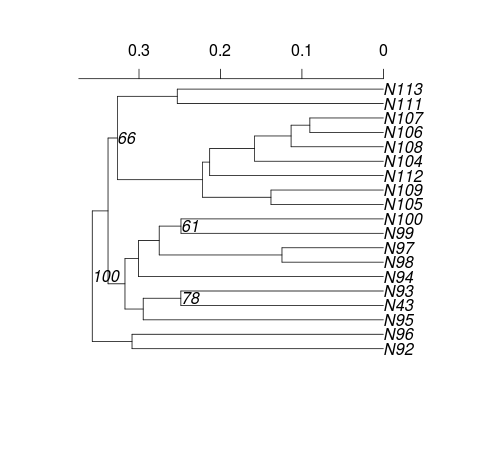
\includegraphics{bruvo_upgma.png}

\includegraphics{poppr_manual-bruvo_tree}

\end{figure}

\subsubsection{Function: greycurve}\label{index:trees:greycurve}
\tab\tab Use this function to display a gradient of grey values based on user-defined parameters. The following functions will display a minimum spanning network that utilize a grey scale to display the weight of the lines (referred to as ``edges") that connect two or more individuals. The darker the line the closer the distance. Since this is based off of a linear grey scale, what happens when you have a distance matrix comprised of values all below 0.2 or all above 0.8? 

With linear grey scaling, it becomes very difficult to detect the differences in these ranges. The following function allows you to visualize and manipulate a gradient from black to white so that you can use it in \textit{poppr}'s msn functions below to maximize the visual differences in your data.

\begin{quote}
Default Command:\\
\texttt{greycurve(glim = c(0, 0.8), gadj = 3, gweight = 1)}
\end{quote}


This function does not return any values. It will print a visual gradient from black to white horizontally. On this gradient, it will plot the adjustment curve (in opposing grey values), yellow horizontal lines bounding the maximum and minimum values, and the equation used to calculate the correction in red. Keep in mind that this is plotting values from zero to one.

%\newpage
First, we'll see what happens when we change the weight parameter.
\setkeys{Gin}{width=\textwidth}
\begin{figure}[h!]
\begin{minipage}[b]{0.45\linewidth}
\centering
\caption{\footnotesize Default for \texttt{greycurve()}, weighted for small values.}
\begin{Schunk}
\begin{Sinput}
> greycurve()
\end{Sinput}
\end{Schunk}
\includegraphics{poppr_manual-greycurve_normal}
\end{minipage}
\hspace{0.5cm}
\begin{minipage}[b]{0.45\linewidth}
\centering
\caption{\footnotesize weighting for large values.}
\begin{Schunk}
\begin{Sinput}
> greycurve(gweight = 2)
\end{Sinput}
\end{Schunk}
\includegraphics{poppr_manual-greywidth_inverse}
\end{minipage}
\end{figure}

Now, we'll see what happens when we change the adjustment parameter (affects the shape of the curve) and the upper and lower limits of the grey scale.

\begin{figure}[h!]
\begin{minipage}[b]{0.45\linewidth}
\centering
\caption{\footnotesize Setting the lower and upper limits and weighting the curve heavily toward smaller values.}
\begin{Schunk}
\begin{Sinput}
> greycurve(glim = c(0.2, 0.9), gadj=15)
\end{Sinput}
\end{Schunk}
\includegraphics{poppr_manual-greycurve_small_heavy}
\end{minipage}
\hspace{0.5cm}
\begin{minipage}[b]{0.45\linewidth}
\centering
\caption{\footnotesize Same as the figure on the left, but weighting heavily toward larger values.}
\begin{Schunk}
\begin{Sinput}
> greycurve(glim = c(0.2, 0.9), gadj=15, gweight=2)
\end{Sinput}
\end{Schunk}
\includegraphics{poppr_manual-greywidth_large_heavy}
\end{minipage}
\end{figure}
\newpage

\subsubsection{Function: bruvo.msn}\label{index:trees:bruvo.msn}
\tab\tab This function will automatically draw a minimum spanning network of MLGs based on Bruvo's distance. It's important to note that this will recalculate Bruvo's distance each time it is run, but the amount of time it takes to run is on the order of seconds. It will return a list containing the network, the populations and the related colors in the network so you can export or redraw it with the legend if you wanted to using the package \textit{igraph} (type \texttt{help("plot.igraph")} for details).
\begin{quote}
Default Command:\\
\texttt{bruvo.msn(pop, replen = c(2), palette = topo.colors, sublist = "All",\\ 
  \tab blacklist = NULL, vertex.label = "MLG", gscale = TRUE, glim = c(0, 0.8),\\ 
  \tab gadj = 3, gweight = 1, wscale = TRUE, ...)
}
\end{quote}
\begin{itemize}
  \item \texttt{pop -} a \texttt{genind} object.
  \item \texttt{replen -} see \texttt{bruvo.dist}, above.
  \item \texttt{palette -} this is a \textbf{function} definining a color palette to use. The default is \texttt{topo.colors}. There are different palettes, which you can search by typing \texttt{?rainbow}. If you want a custom color palette, an easy way is to use the function \texttt{colorRampPalette}.
  \item \texttt{sublist -} The populations you wish to analyze. This defaults to ``All". See section \ref{data.manip:divide:popsub} for details.
  \item \texttt{blacklist -} Populations you do not want to include in the graph. See section \ref{data.manip:divide:popsub} for details.
  \item \texttt{vertex.label -} This is an option that is passed on to \textit{igraph}'s \texttt{plot} function. \textit{Poppr} has added two arguments specific to \textit{poppr}. If you want to label the graph with the multilocus genotypes from the whole data set, use the argument \texttt{vertex.label = "mlg"}. If you want to display the representative individual names, you can use the argument \texttt{vertex.label = "inds"}. I say representative individual names because, only one representative from each MLG will be present in the clone corrected data set used to calculate the distance. For no labels, you can choose \texttt{vertex.label = NA}. 
  \item \texttt{gscale -} If this is set to \texttt{TRUE}, the edge color will be converted to greyscale based on Bruvo's distance. If two nodes are closely related, the edge will appear darker. The limits of the scale can be set by the argument \texttt{glim}. If this is set to \texttt{FALSE}, all edge colors will be black. 
  \item \texttt{glim -} This is a vector of numbers between 0 and 1. This lets you set the limits of the grey scaling based on R's internal \texttt{grey} function. For example, if you wanted a maximum of 50\% white saturation (for use if you have distantly related nodes) and a minimum of 1\%, you would use \texttt{glim = c(0.01, 0.5)}. 
  \item \texttt{gadj -} This is an integer greater than zero used to adjust the scaling factor for the grey curve. Since very small changes in the grey scale are not easily precieved, it's useful to be able to adjust the grey scale to be able to show you the weights of each edge. For example, a population with most weights less than 0.3, you might want to set \texttt{gadj = 10} to exaggerate the grey scale. 
  \item \texttt{gweight -} If \texttt{gweight = 1}, the grey scale adjustment will be weighted towards separating out smaller values of Bruvo's distance. If \texttt{gweight = 2}, the grey scale ajustment will be weighted towards separating out larger values of Bruvo's distance.
  \item \texttt{wscale -} If this is set to \texttt{TRUE}, edge widths will be displayed corresponding to Bruvo's distance in that thicker edges will represent a smaller distance between nodes. If this is set to \texttt{FALSE}, all edges will be set to a width of 2. 
  \item \texttt{... -} This is a placeholder for any other arguments that you want to supply to \textit{igraph}. Useful arguments are \texttt{vertex.label.cex} to adjust the size of the labels, \texttt{vertex.label.dist} to adjust the position of the labels, and \texttt{vertex.label.color} to adjust the color of the labels.
\end{itemize}

Often, minimum spanning networks are the preferred way to visualize Bruvo's distance. \textit{Poppr} offers an easy way to plot these. For a demonstration, let's analyze a simulated data set of 50 individuals from populations that reproduce at a 99.9\% rate of clonal reproduction.

\begin{Schunk}
\begin{Sinput}
> data(partial_clone)
> set.seed(9005)
> pc.msn <- bruvo.msn(partial_clone, replen=rep(1, 10), vertex.label.cex=0.7, 
+           vertex.label.dist=-0.5, palette=colorRampPalette(c("blue", "yellow")))
\end{Sinput}
\end{Schunk}
\setkeys{Gin}{width=0.8\textwidth}
\begin{figure}[ht!]
  \centering
  \caption{\footnotesize Minimum Spanning Network representing 4 simulated populations. Each node represents a different multi locus genotype (MLG). Node sizes and colors correspond to the number of individuals and population membership, respectively. Edge thickness and color are proportional to Bruvo's distance. Edge lengths are arbitrary.}
  \label{mst_bruvo}
\includegraphics{poppr_manual-bruvo_msn}
\end{figure}
\setkeys{Gin}{width=0.5\textwidth}

The output, as mentioned earlier, is a list containing the graph constructed via the \textit{igraph} package, a vector of the population names and a vector of colors representing the populations.
\begin{Schunk}
\begin{Sinput}
> library(igraph)
> pc.msn
\end{Sinput}
\begin{Soutput}
$graph
IGRAPH UNW- 26 25 -- 
+ attr: name (v/c), size (v/n), shape (v/c), pie (v/x), pie.color (v/x), label
  (v/c), weight (e/n), color (e/c), width (e/n)

$populations
[1] "1" "2" "3" "4"

$colors
[1] "#0000FF" "#5555AA" "#AAAA55" "#FFFF00"
\end{Soutput}
\end{Schunk}

Note that the thickness of the edges (the lines that are connecting the dots) is representative of relatedness between individuals, but the lengths do not necessarily mean anything due to the fact that with a larger data sets, displaying lengths proportional to relatedness would be impossible to draw on a 2D surface. Interpreting these data would show that MLG 9 has 5 individuals from all four populations and that it is most closely related to MLG 7, whereas the most distantly related connection exists between MLG 25 and MLG 26.
\newpage
Since a graph can be represented in many ways, you might want to play around with different layouts using the \texttt{layout()} function in \textit{igraph}. Type \texttt{help("layout", package = igraph)} for details. Below is the code for reconstructing the previous graph using the output:
\begin{Schunk}
\begin{Sinput}
> set.seed(9005)
> library(igraph)
> plot(pc.msn$graph, vertex.size = V(pc.msn$graph)$size * 3, vertex.label.cex=0.7, 
+      vertex.label.dist=-0.5,)
> legend(-1.55, 1, bty = "n", cex = 0.75, legend = pc.msn$populations, 
+        title = "Populations", fill = pc.msn$colors, border = NULL)
\end{Sinput}
\end{Schunk}

\subsubsection{Function: poppr.msn}\label{index:trees:poppr.msn}

\tab\tab Use this function to draw a minimum spanning network from your data set and a distance matrix derived from your data set. Since there are hundreds of distances that can be calculated for genetic data, and since I want to be able to graduate at some point in this decade, functions to automatically calculate distances and draw the minimum spanning networks will be few and far between. This function is an attempt to meet the user halfway and draw a minimum spanning network provided that the user has supplied two things:
\begin{enumerate}
  \item A distance matrix over all individuals.
  \item The original data set containing demographic information.
\end{enumerate}

That's it. For the most part, this function is functionally the same as \texttt{bruvo.msn}, except that instead of being exclusive to microsatellite markers, you can now visualize distances in any marker type provided that you have the two items listed above.

\begin{quote}
Default Command:\\
\texttt{poppr.msn(pop, distmat, palette = topo.colors, sublist = "All",\\ 
  \tab blacklist = NULL, vertex.label = "MLG", gscale = TRUE, glim = c(0, 0.8),\\ 
  \tab gadj = 3, gweight = 1, wscale = TRUE, ...)
}
\end{quote}
\begin{itemize}
  \item \texttt{pop -} a \texttt{genind} object.
  \item \texttt{distmat -} a dissimilarity distance matrix derived from your data with distances between zero and one.
  \item \texttt{palette -} this is a \textbf{function} definining a color palette to use. The default is \texttt{topo.colors}. There are different palettes, which you can search by typing \texttt{?rainbow}. If you want a custom color palette, an easy way is to use the function \texttt{colorRampPalette}.
  \item \texttt{sublist -} The populations you wish to analyze. This defaults to ``All".
  \item \texttt{blacklist -} Populations you do not want to include in the graph.
  \item \texttt{vertex.label -} This is an option that is passed on to \textit{igraph}'s \texttt{plot} function. \textit{Poppr} has added two arguments specific to \textit{poppr}. If you want to label the graph with the multilocus genotypes from the whole data set, use the argument \texttt{vertex.label = "mlg"}. If you want to display the representative individual names, you can use the argument \texttt{vertex.label = "inds"}. I say representative individual names because, only one representative from each MLG will be present in the clone corrected data set used to calculate the distance. For no labels, you can choose \texttt{vertex.label = NA}. 
  \item \texttt{gscale -} If this is set to \texttt{TRUE}, the edge color will be converted to greyscale based on the distance. If two nodes are closely related, the edge will appear darker. The limits of the scale can be set by the argument \texttt{glim}. If this is set to \texttt{FALSE}, all edge colors will be black. 
  \item \texttt{glim -} This is a vector of numbers between 0 and 1. This lets you set the limits of the grey scaling based on R's internal \texttt{grey} function. For example, if you wanted a maximum of 50\% white saturation (for use if you have distantly related nodes) and a minimum of 1\%, you would use \texttt{glim = c(0.01, 0.5)}. 
  \item \texttt{gadj -} This is an integer greater than zero used to adjust the scaling factor for the grey curve. Since very small changes in the grey scale are not easily precieved, it's useful to be able to adjust the grey scale to be able to show you the weights of each edge. For example, a population with most weights less than 0.3, you might want to set \texttt{gadj = 10} to exaggerate the grey scale. 
  \item \texttt{gweight -} If \texttt{gweight = 1}, the grey scale adjustment will be weighted towards separating out smaller values of the distance. If \texttt{gweight = 2}, the grey scale ajustment will be weighted towards separating out larger values of Bruvo's distance.
  \item \texttt{wscale -} If this is set to \texttt{TRUE}, edge widths will be displayed corresponding to Bruvo's distance in that thicker edges will represent a smaller distance between nodes. If this is set to \texttt{FALSE}, all edges will be set to a width of 2. 
  \item \texttt{... -} This is a placeholder for any other arguments that you want to supply to \textit{igraph}. Useful arguments are \texttt{vertex.label.cex} to adjust the size of the labels, \texttt{vertex.label.dist} to adjust the position of the labels, and \texttt{vertex.label.color} to adjust the color of the labels.
\end{itemize}

Since we have the ability, let's visualize the \textit{A. euteiches} data set \cite{Grunwald:2006}.
\begin{Schunk}
\begin{Sinput}
> data(Aeut)
> A.dist <- diss.dist(Aeut)
> set.seed(9005)
> A.msn <- poppr.msn(Aeut, A.dist, vertex.label=NA, palette=rainbow, gadj=15)
\end{Sinput}
\end{Schunk}

\setkeys{Gin}{width=0.8\textwidth}
\begin{figure}[ht!]
  \centering
  \caption{\footnotesize Minimum Spanning Network representing 4 simulated populations. Each node represents a different multi locus genotype (MLG). Node sizes and colors correspond to the number of individuals and population membership, respectively. Edge thickness and color are proportional to Bruvo's distance. Edge lengths are arbitrary.}
  \label{mst_poppr}
\includegraphics{poppr_manual-poppr_msn_fig}
\end{figure}
\setkeys{Gin}{width=0.5\textwidth}
\newpage
%\subsubsection{Gory details} 
%%%%%%%%%%%%%%%%%%%%%%%%%%%%%%%%%%%%%%%%%%%%%%%%%%%%%%%%%%%%%%%%%%%%%%%%%%%%%%%%
%%%%%%%%%%%%%%%%%%%%%%%%%%%%%%%%%%%%%%%%%%%%%%%%%%%%%%%%%%%%%%%%%%%%%%%%%%%%%%%%
%%%%%%%%%%%%%%%%%%%%%%%%%%%%%%%%%%%%%%%%%%%%%%%%%%%%%%%%%%%%%%%%%%%%%%%%%%%%%%%%
\section{I know what you did last summary table \{diversity table\}}\label{summary}

\tab\tab Remember the summary function that you used to get all the diversity statistics in section \ref{intro:qstart}? In this section, we will flesh out all that you can do with this function. This was the very first function that was written for \textit{poppr} to make it easy for the user to manipulate and summarize the data in one function.
\subsection{Function: poppr}\label{summary:poppr}

\tab\tab This function is quite daunting with all its possibilities. You have the option to subset your data for specific populations, correct for missing data, and clone correct. With each of these possibilities, comes the need to provide all the arguments for their various functions.
\begin{quote}
Default Command:\\
\texttt{poppr(pop, total = TRUE, sublist = c("ALL"), blacklist = c(NULL), sample = 0,\\ 
        \tab method = 1, missing = "ignore", cutoff = 0.05, quiet = FALSE, \\
        \tab clonecorrect = FALSE, hier = c(1), dfname = "population\_hierarchy", \\
        \tab hist = TRUE, minsamp = 10)}
\end{quote}
\begin{itemize}
  \item \texttt{pop -} A \texttt{genind} object.
  \item \texttt{total -} This is also a synonym for ``pooled". This will calculate all diversity statistics on the entire data set if set to \texttt{TRUE} or if there is no population structure.
  \item \emph{popsub functions:} See section \ref{data.manip:divide}
  \begin{description}
    \item[sublist -] A list of populations you want to include in your analysis.
    \item[blacklist -] A list of populations you want to exclude from your analysis.
  \end{description}
  \item \emph{shufflepop functions:} See section \ref{data.manip:shuffle} \\ Note that this only affects the calculation for $I_A$ and $\bar r_d$.
  \begin{description}
    \item[sample -] The number of samples you desire (eg. 999)
    \item[method -] Which sampling method? 1: multilocus, 2: permute, 3: parametric bootstrap, 4: non-parametric bootstrap.
  \end{description}
  \item \emph{missingno functions:} See Section \ref{data.manip:missing} \\ Note that all analyses in this function ignore/impute missing data by default.
    \begin{description}
      \item[missing -] How to deal with missing data. This feeds into the \texttt{type} flag of \texttt{missingno}.
      \item[cutoff -] Allowable percentage of missing data per genotype or locus.
    \end{description}
  \item \texttt{quiet -} If set to \texttt{TRUE}, nothing will be printed to the screen as the sampling progresses. If \texttt{FALSE} (default) a progress bar will be produced.
  \item \emph{clonecorrect functions:} See section \ref{data.manip:cc}
  \begin{description}
    \item[clonecorrect -] if this is set to \texttt{TRUE}, then you will need to set the next two parameters.
    \item[hier -] A list of the population hierarchy, or names of columns in the data frame noted below.
    \item[dfname -] A data frame in the \texttt{@other} slot of the \texttt{genind} object containing all of the population factors in different columns. For an example, see sections \ref{data.manip:hier} and \ref{data.manip:cc}.
    \item[keep -] A vector of integers as indexes for the \texttt{hier} flag indicating which levels of the hierarchy you want to analyze. See section \ref{data.manip:cc} for details. 
  \end{description}
  \item \texttt{hist -} if \texttt{TRUE}, a histogram of distributions of $I_A$ and $\bar r_d$ will be displayed with each population if there is sampling.
  \item \texttt{minsamp -} The minimum number of individuals you want to use to calculate the expected number of MLGs. The default is set to 10.
\end{itemize}

This function produces a table that contains the population name, number of individuals observed, number of MLGs observed, number of MLGs expected at the lowest common sampling size within the data set \cite{Hurlbert:1971} \cite{Heck:1975}, the Shannon-Wiener index \cite{Shannon:1948}, Stoddart and Taylor's index for expected MLGs \cite{Stoddart:1988}, Nei's 1987 genotypic diversity \cite{Nei:1978}, evenness \cite{Pielou:1975}\cite{Ludwig:1988}\cite{Grunwald:2003}, the index of association \cite{Brown:1980}\cite{Smith:1993}, the standardized index of association \cite{Agapow:2001}, and the file name. Most of these indices are calculated by converting the population into an MLG table with \texttt{mlg.table} (see section \ref{mlg:table}) and using the \textit{vegan} package's \texttt{diversity} function (To see details, type \texttt{?vegan::diversity} into the R console).

To begin, let's revisit our example data set of \textit{Aphanomyces euteiches} \cite{Grunwald:2006}.
\begin{Schunk}
\begin{Sinput}
> data(Aeut)
> poppr(Aeut)
\end{Sinput}
\begin{Soutput}
| Athena 
| Mt. Vernon 
| Total 
         Pop   N MLG   eMLG    SE     H      G  Hexp   E.5     Ia rbarD        File
1     Athena  97  70 65.981 1.246 4.063 42.193 0.986 0.721  2.906 0.072 rootrot.csv
2 Mt. Vernon  90  50 50.000 0.000 3.668 28.723 0.976 0.726 13.302 0.282 rootrot.csv
3      Total 187 119 68.453 2.989 4.558 68.972 0.991 0.720 14.371 0.271 rootrot.csv
\end{Soutput}
\end{Schunk}
OK, so we were able to get a table out of this. Now let's see what happens when we do some sampling to see if this is reproducing clonally or not (for simplicity's sake, we will stick with the default multilocus sampling method). We will turn quiet on and the histogram off to save space.
\begin{Schunk}
\begin{Sinput}
> poppr(Aeut, sample=999, hist=FALSE, quiet=TRUE)
\end{Sinput}
\end{Schunk}
\begin{Schunk}
\begin{Soutput}
         Pop   N MLG   eMLG    SE     H      G  Hexp   E.5     Ia  p.Ia rbarD  p.rD
1     Athena  97  70 65.981 1.246 4.063 42.193 0.986 0.721  2.906 0.001 0.072 0.001
2 Mt. Vernon  90  50 50.000 0.000 3.668 28.723 0.976 0.726 13.302 0.001 0.282 0.001
3      Total 187 119 68.453 2.989 4.558 68.972 0.991 0.720 14.371 0.001 0.271 0.001
         File
1 rootrot.csv
2 rootrot.csv
3 rootrot.csv
\end{Soutput}
\end{Schunk}
From now on, we'll set \texttt{quiet = TRUE} to save space on our vignette. Let's clone correct at different levels to see if that affects the index of association. First, we'll clone correct at the sub population level.
\begin{Schunk}
\begin{Sinput}
> poppr(Aeut, sample=999, clonecorrect=TRUE, hier=c("Pop","Subpop"), 
+       dfname="population_hierarchy", quiet=TRUE, hist=FALSE)
\end{Sinput}
\end{Schunk}
\begin{Schunk}
\begin{Soutput}
         Pop   N MLG   eMLG    SE     H      G  Hexp   E.5     Ia  p.Ia rbarD  p.rD
1     Athena  76  70 60.621 1.017 4.221 65.636 0.998 0.963  2.535 0.001 0.062 0.001
2 Mt. Vernon  65  50 50.000 0.000 3.796 36.739 0.988 0.821 14.310 0.001 0.298 0.001
3      Total 141 119 59.629 1.854 4.705 96.980 0.997 0.876 13.802 0.001 0.260 0.001
         File
1 rootrot.csv
2 rootrot.csv
3 rootrot.csv
\end{Soutput}
\end{Schunk}
And at the population level.
\begin{Schunk}
\begin{Sinput}
> poppr(Aeut, sample=999, clonecorrect=TRUE, hier="Pop", 
+       dfname="population_hierarchy", quiet=TRUE, hist=FALSE)
\end{Sinput}
\end{Schunk}
\begin{Schunk}
\begin{Soutput}
         Pop   N MLG   eMLG    SE     H       G Hexp   E.5     Ia  p.Ia rbarD  p.rD
1     Athena  70  70 50.000 0.000 4.248  70.000    1 1.000  2.438 0.001 0.060 0.001
2 Mt. Vernon  50  50 50.000 0.000 3.912  50.000    1 1.000 13.856 0.001 0.285 0.001
3      Total 120 119 49.828 0.377 4.776 118.033    1 0.995 12.497 0.001 0.234 0.001
         File
1 rootrot.csv
2 rootrot.csv
3 rootrot.csv
\end{Soutput}
\end{Schunk}
As you can see, clone correction doesn't always have to involve creation of new data sets!

You might notice that the P-values for both $I_A$ and $\bar r_d$ are often equal to each other. This is due to the default sampling method \cite{Agapow:2001}. Here, we show examples where they are not equal.
\begin{Schunk}
\begin{Sinput}
> set.seed(2001)
> poppr(nancycats, sublist=5:6, total=FALSE, sample=999, method=3, quiet=TRUE, hist=FALSE)
\end{Sinput}
\end{Schunk}
\begin{Schunk}
\begin{Soutput}
  Pop  N MLG eMLG SE     H  G Hexp E.5     Ia  p.Ia  rbarD  p.rD                     File
1   5 15  15   11  0 2.708 15    1   1 -0.048 0.599 -0.006 0.599 truenames(nancycats)$tab
2   6 11  11   11  0 2.398 11    1   1  0.334 0.064  0.043 0.065 truenames(nancycats)$tab
\end{Soutput}
\end{Schunk}
The reason why the P-values would be different is described at the end of section \ref{index:iard:ia}. The differences in P-values are normally not very far off. It's important to note this because of what can happen in extremely clonal populations. You can end up with a large enough sample size consisting of very few MLGs. Upon shuffling, you find that there are very few values of $I_A$ and $\bar r_d$ that can be obtained. Observe with this simulated data set:
\begin{Schunk}
\begin{Sinput}
> set.seed(2004)
> poppr(system.file("files/simulated.dat", package="poppr"), sample=999, method=1, quiet=TRUE)
\end{Sinput}
\end{Schunk}
\begin{Schunk}
\begin{Soutput}
    Pop   N MLG eMLG SE     H    G  Hexp   E.5   Ia p.Ia rbarD p.rD          File
1 Total 100   6    6  0 1.235 2.79 0.648 0.735 0.05 0.09 0.061 0.09 simulated.dat
\end{Soutput}
\end{Schunk}
\begin{figure}[h!]
  \centering
  \caption{\footnotesize Output of multilocus-style sampling. Note the multi-modal distribution.}
  \label{simulated_dist_fig}
  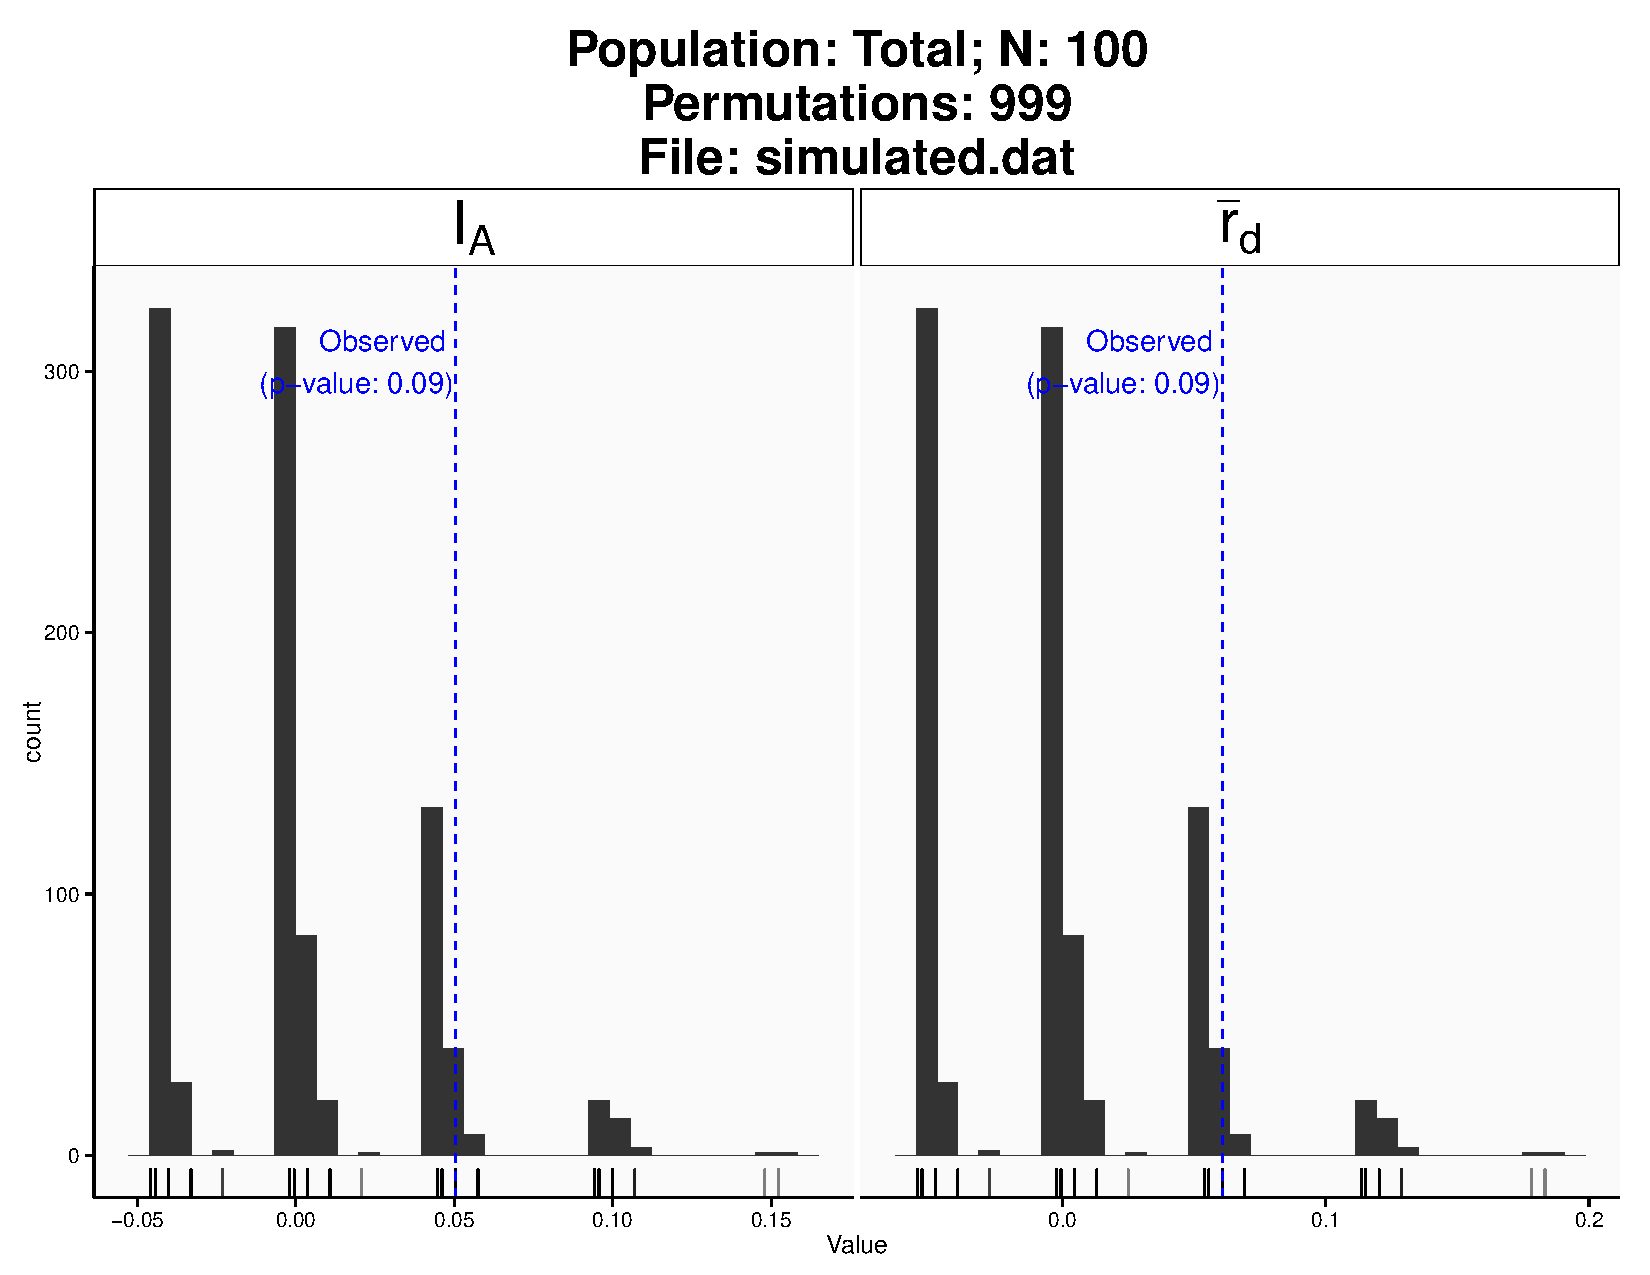
\includegraphics{simulated_dist_fig.png}
% <<fig=TRUE, echo=FALSE, resolution=300, figs.only=TRUE, width=8, height=8>>=
% set.seed(2004)
% der <- poppr(system.file("files/simulated.dat", package="poppr"), sample=999, method=1, quiet=TRUE, hist=TRUE)
% @
\end{figure}
\newpage

Take a look a these two histograms. The number of ways you can recombine the data with the default sampling method is very small. Other sampling methods could give a more theoretical distribution. Let's try the parametric bootstrap (For details, see section \ref{data.manip:shuffle}).
\begin{figure}[h!]
  \centering
  \caption{\footnotesize Output for parametric bootstrap sampling.}
  \label{simulated_param_fig}
  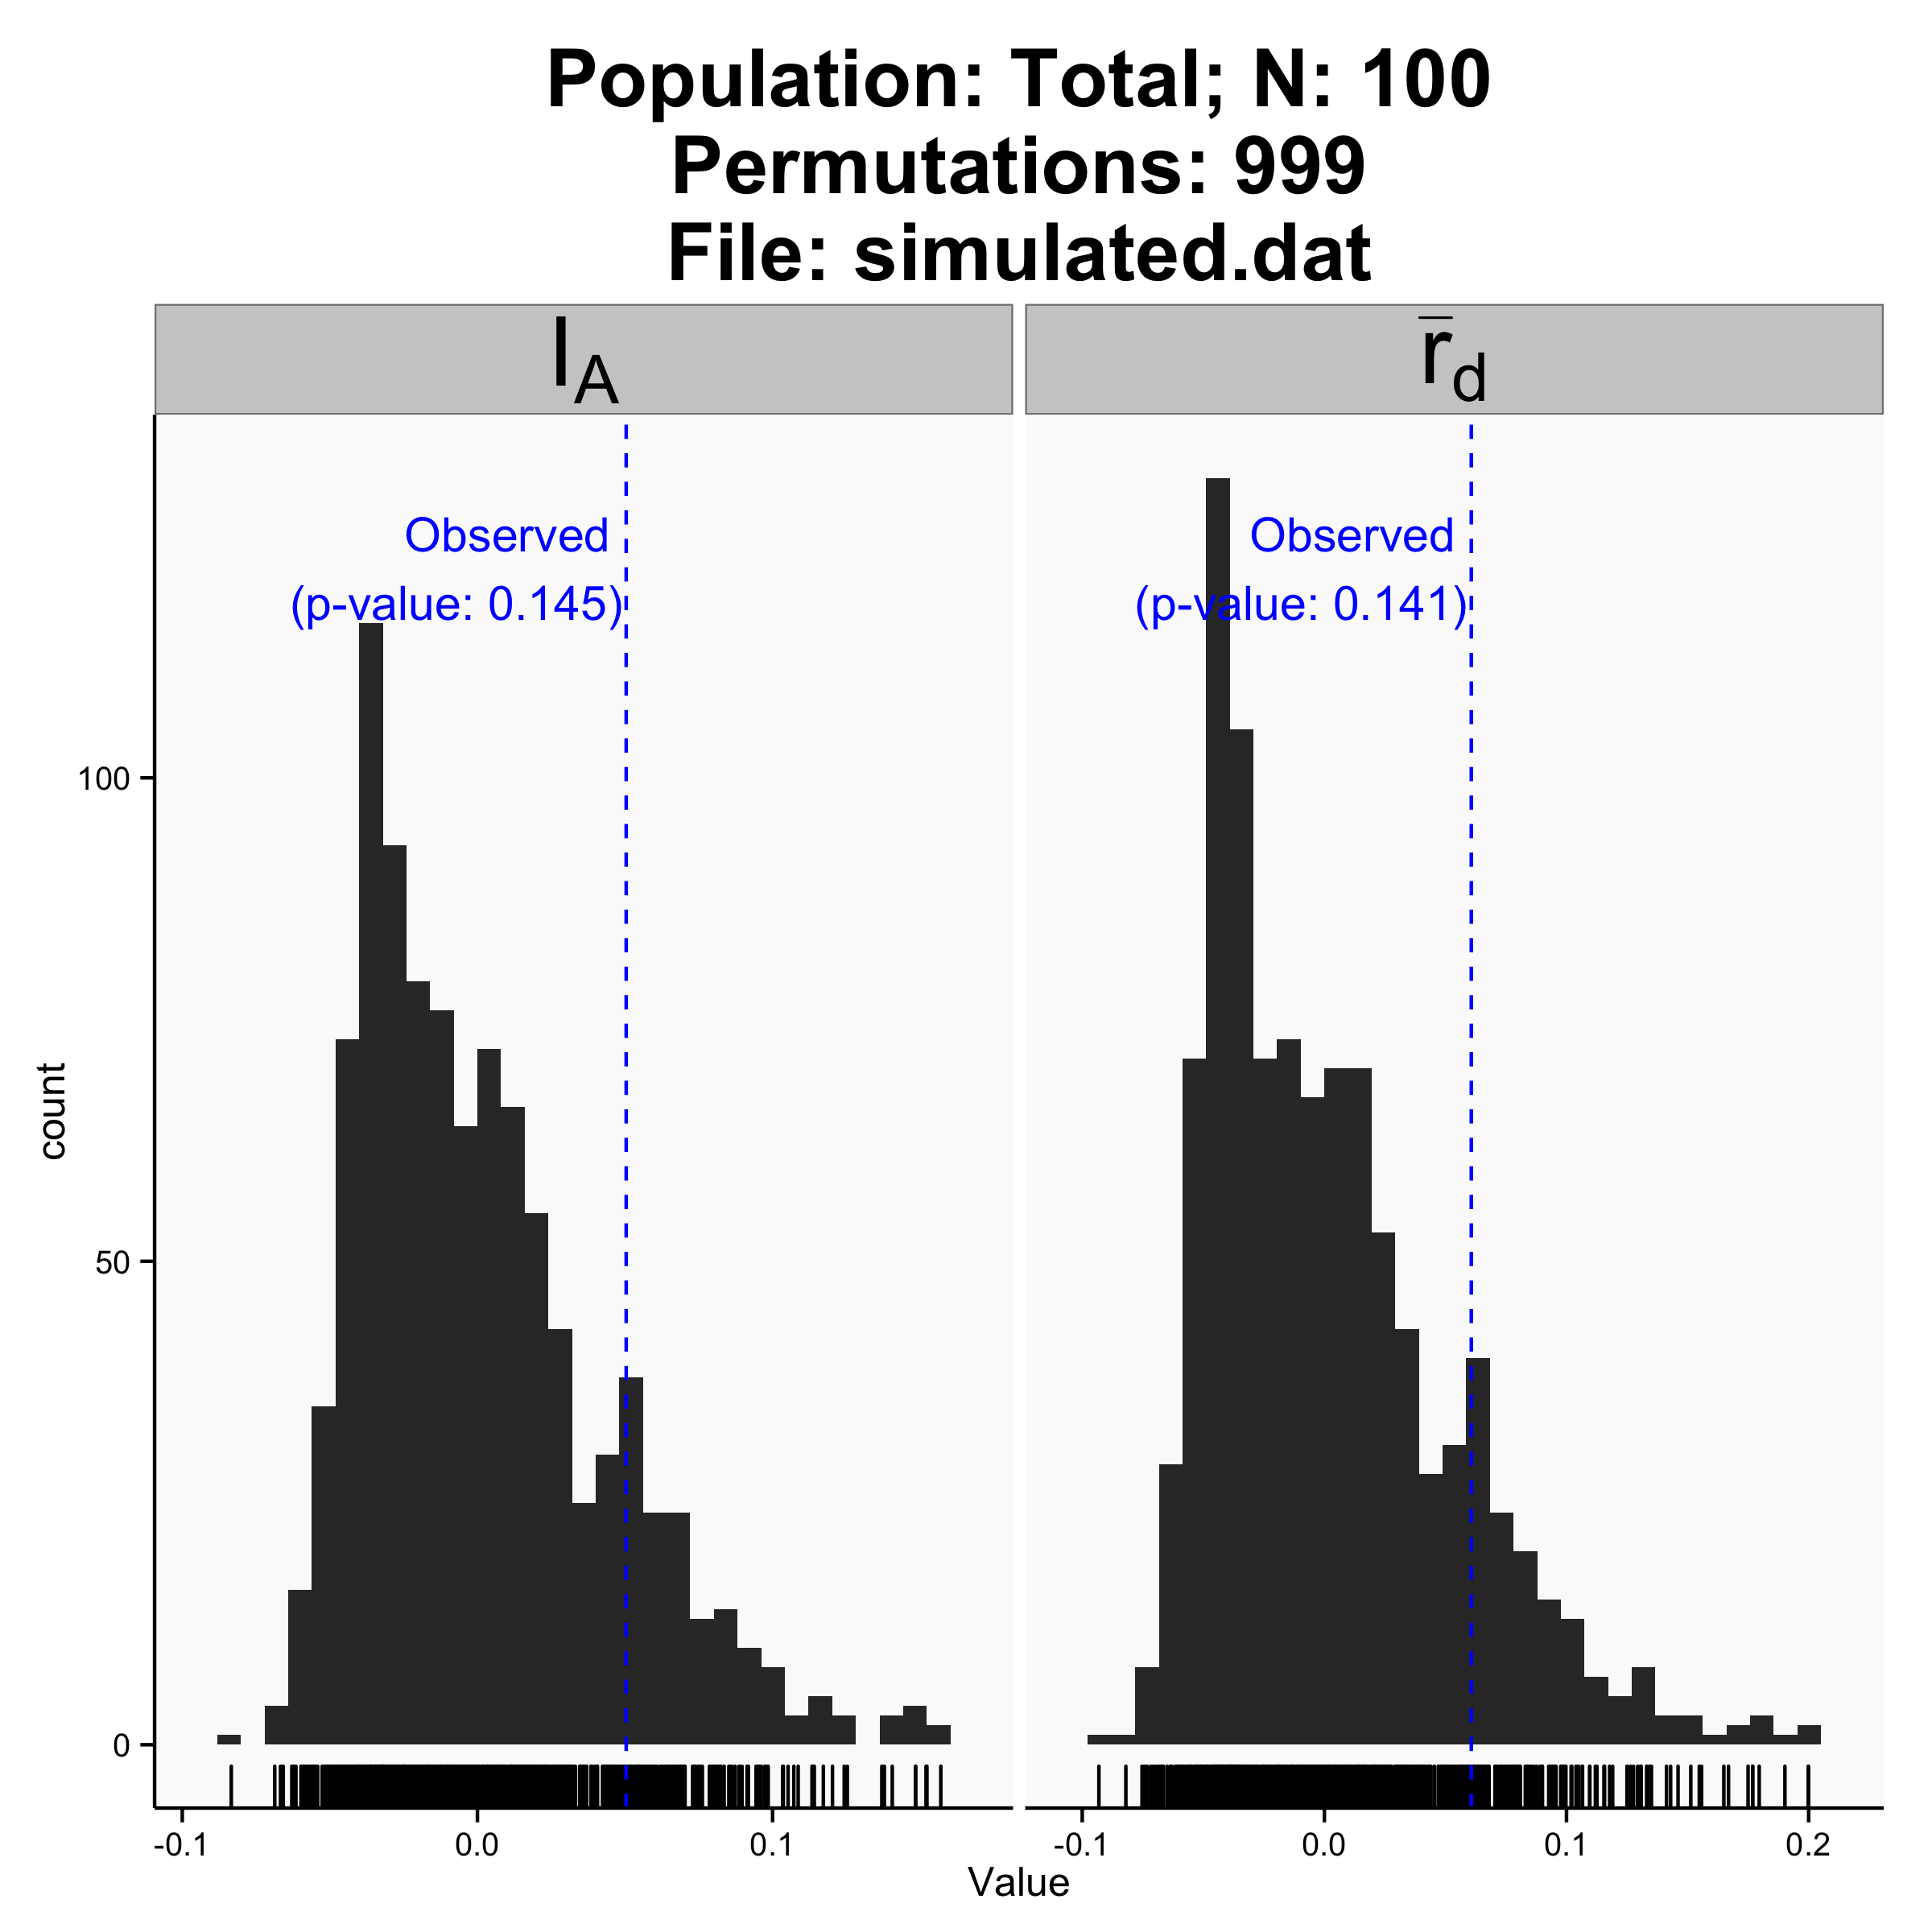
\includegraphics{simulated_param_fig.png}
% <<fig=TRUE, echo=FALSE, resolution=300, figs.only=TRUE, width=8, height=8>>=
% set.seed(2004)
% der <- poppr(system.file("files/simulated.dat", package="poppr"), sample=999, method=3, quiet=TRUE)
% @
\end{figure}

As you can see, the distribution is much closer to a distribution we would expect if this were a small sample of a larger population. 


%%%%%%%%%%%%%%%%%%%%%%%%%%%%%%%%%%%%%%%%%%%%%%%%%%%%%%%%%%%%%%%%%%%%%%%%%%%%%%%%
%%%%%%%%%%%%%%%%%%%%%%%%%%%%%%%%%%%%%%%%%%%%%%%%%%%%%%%%%%%%%%%%%%%%%%%%%%%%%%%%
%%%%%%%%%%%%%%%%%%%%%%%%%%%%%%%%%%%%%%%%%%%%%%%%%%%%%%%%%%%%%%%%%%%%%%%%%%%%%%%%
\section{Appendix}\label{appendix}
\subsection{Algorithmic Details}\label{appendix:algorithm}
\subsubsection{$I_A$ and $\bar r_d$}\label{appendix:algorithm:iard}

\tab \tab The index of association was originally developed by A.H.D. Brown analyzing population structure of wheat \cite{Brown:1980}. It has been widely used as a tool to detect clonal reproduction within populations \cite{Smith:1993}. Populations whose members are undergoing sexual reproduction, whether it be selfing or out-crossing, will produce gametes via meiosis, and thus have a chance to shuffle alleles in the next generation. Populations whose members are undergoing clonal reproduction, however, generally do so via mitosis. This means that the most likely mechanism for a change in genotype is via mutation. The rate of mutation varies from species to species, but it is rarely sufficiently high to approximate a random shuffling of alleles. The index of association is a calculation based on the ratio of the variance of the raw number of differences between individuals and the sum of those variances over each locus \cite{Smith:1993}. You can also think of it as the observed variance over the expected variance. If they  are the same, then the index is zero after subtracting one (from Maynard-Smith, 1993 \cite{Smith:1993}):
\beq
\label{eq:I_A}
I_A = \frac{V_O}{V_E}-1
\eeq
Since the distance is more or less a binary distance, any sort of marker can be used for this analysis. In the calculation, phase is not considered, and any difference increases the distance between two individuals. Consider the genotypes of the dummy data frame we created earlier:
\begin{Schunk}
\begin{Soutput}
   locus1  locus2  locus3
1 101/101 201/201 301/302
2 102/103 202/203 301/303
3 102/102 203/204 304/305
\end{Soutput}
\end{Schunk}
Now, consider the first locus represented in the genind object:
\begin{Schunk}
\begin{Soutput}
  L1.1 L1.2 L1.3
1    1  0.0  0.0
2    0  0.5  0.5
3    0  1.0  0.0
\end{Soutput}
\end{Schunk}
Remember that each column represents a different allele and that each entry in the table represents the fraction of the genotype made up by that allele at that locus. Notice also that the sum of the rows all equal one. \textit{Poppr} uses this to calculate distances by simply taking the sum of the absolute values of the differences between rows.

The calculation for the distance between two individuals at a single locus with $a$ allelic states and a ploidy of $k$ is as follows\footnote{Individuals with Presence / Absence data will have the $k/2$ term dropped.}:
\beq
\label{eq:ia_d}
d = \displaystyle \frac{k}{2}\sum_{i=1}^{a} \mid ind_{Ai} - ind_{Bi}\mid
\eeq
\begin{Schunk}
\begin{Sinput}
> abs(dfg@tab[1, 1:3] - dfg@tab[2, 1:3])
\end{Sinput}
\begin{Soutput}
L1.1 L1.2 L1.3 
 1.0  0.5  0.5 
\end{Soutput}
\begin{Sinput}
> abs(dfg@tab[1, 1:3] - dfg@tab[3, 1:3])
\end{Sinput}
\begin{Soutput}
L1.1 L1.2 L1.3 
   1    1    0 
\end{Soutput}
\begin{Sinput}
> abs(dfg@tab[2, 1:3] - dfg@tab[3, 1:3])
\end{Sinput}
\begin{Soutput}
L1.1 L1.2 L1.3 
 0.0  0.5  0.5 
\end{Soutput}
\end{Schunk}
As you can see, these values of $d$ at locus one add up to 2, 2, and 1, respectively.

To find the total number of differences between two individuals over all loci, you just take $d$ over $m$ loci, a value we'll call $D$:

\beq
\label{eq:ia_D}
D = \displaystyle \sum_{i=1}^{m} d_i
\eeq

These values are calculated over all possible combinations of individuals in the data set, ${n \choose 2}$ after which you end up with ${n \choose 2}\cdot{}m$ values of $d$ and ${n \choose 2}$ values of $D$.
Calculating the observed variances is fairly straightforward (modified from Agapow and Burt, 2001) \cite{Agapow:2001}:

\beq
\label{eq:V_O}
V_O = \frac{\displaystyle \sum_{i=1}^{n \choose 2} D_{i}^2 - \frac{(\displaystyle\sum_{i=1}^{n \choose 2} D_{i})^2}{{n \choose 2}}}{{n \choose 2}}
\eeq

Calculating the expected variance is the sum of each of the variances of the individual loci. The calculation at a single locus, $j$ is the same as the previous equation, substituting values of $D$ for $d$ \cite{Agapow:2001}:

\beq
\label{eq:var_j}
var_j = \frac{\displaystyle \sum_{i=1}^{n \choose 2} d_{i}^2 - \frac{(\displaystyle\sum_{i=1}^{n \choose 2} d_i)^2}{{n \choose 2}}}{{n \choose 2}}
\eeq

The expected variance is then the sum of all the variances over all $m$ loci \cite{Agapow:2001}:

\beq
\label{eq:V_E}
V_E = \displaystyle \sum_{j=1}^{m} var_j
\eeq

Now you can plug the sums of equations (\ref{eq:V_O}) and (\ref{eq:V_E}) into equation (\ref{eq:I_A}) to get the index of association.
Of course, Agapow and Burt showed that this index increases steadily with the number of loci, so they came up with an approximation that is widely used, $\bar r_d$ \cite{Agapow:2001}. For the derivation, see the manual for \textit{multilocus}. The equation is as follows, utilizing equations (\ref{eq:V_O}), (\ref{eq:var_j}), and (\ref{eq:V_E}) \cite{Agapow:2001}:

\beq
\label{eq:r_d}
\bar{r_d} = \frac{V_O - V_E}
{2\displaystyle \sum_{j=1}^{m}\displaystyle \sum_{k \neq j}^{m}\sqrt{var_j\cdot{}var_k}}
\eeq

%%%%%%%%%%%%%%%%%%%%%%%%%%%%%%%%%%%%%%%%%%%%%%%%%%%%%%%%%%%%%%%%%%%%%%%%%%%%%%%%
\subsubsection{Bruvo's distance}\label{appendix:algorithm:bruvo}

\tab \tab Bruvo's distance between two individuals calculates the minimum distance across all combinations of possible pairs of alleles at a single locus and then averaging that distance across all loci \cite{Bruvo:2004}. The distance between each pair of alleles is calculated as \cite{Bruvo:2004}:

\beq
\label{eq:m_x}
m_x = 2^{-\mid x \mid}
\eeq

\beq
\label{eq:d_a}
d_a = 1 - m_x
\eeq

Where $x$ is the number of steps between each allele. So, let's say we were comparing two haploid $(k = 1)$ individuals with alleles 228 and 244 at a locus that had a tetranucleotide repeat pattern (CATG$)^n$. The number of steps for each of these alleles would be $228/4 = 57$ and $244/4 =61$, respectively. The number of steps between them is then $\mid 57 - 61 \mid = 4$. Bruvo's distance at this locus between these two individuals is then $1-2^{-4} = 0.9375$. For samples with higher ploidy ($k$), there would be $k$ such distances of which we would need to take the sum \cite{Bruvo:2004}.

\beq
\label{eq:s_i}
s_i = \displaystyle \sum_{a=1}^{k} d_a
\eeq

Unfortunately, it's not as simple as that since we do not assume to know phase. Because of this, we need to take all possible combinations of alleles into account. This means that we will have $k^2$ values of $d_a$, when we only want $k$. How do we know which $k$ distances we want? We will have to invoke parsimony for this and attempt to take the minimum sum of the alleles, of which there are $k!$ possibilities \cite{Bruvo:2004}:

\beq
\label{eq:d_l}
d_l = \frac{\left(\displaystyle \min_{i \dotsc k!} s_i\right)}{k}
\eeq

Finally, after all of this, we can get the average distance over all loci \cite{Bruvo:2004}. 

\beq
\label{eq:D}
D = \frac{\displaystyle \sum_{i=1}^l d_i}{l}
\eeq

This is calculated over all possible combinations of individuals and results in a lower triangle distance matrix over all individuals. 

\subsection{Exporting Graphics}\label{appendix:graphics}
\tab\tab R has the ability to produce nice graphics from most any type of data, but to get these graphics into a report, presentation, or manuscript can be a bit challenging. It's no secret that the R Documentation pages are a little difficult to interpret, so I will give the reader here a short example on how to export graphics from R. Note that any code here that will produce images will also be present in other places in this vignette. The default installation of the R GUI is quite minimal, and for an easy way to manage your plots and code, I strongly encourage the user to use Rstudio \url{http://www.rstudio.com/}.

\subsubsection{Basics}\label{appendix:graphics:basics}
\tab\tab Before you export graphics, you have to ask yourself what they will be used for. If you want to use the graphic for a website, you might want to opt for a low-resolution image so that it can load quickly. With printing, you'll want to make sure that you have a scalable or at least a very high resolution image. Here, I will give some general guidelines for graphics (note that these are merely suggestions, not defined rules).
\begin{itemize}
  \item \textbf{What you see is not always what you get} I have often seen presentations where the colors were too light or posters with painfully pixellated graphs. Think about what you are going to be using a graphic for and how it will appear to the intended audience given the media type.
  \item \textbf{$\geq$ 300 dpi unless its for a web page} For any sort of printed material that requires a raster based image, 300dpi (dots per inch) is the absolute minimum resolution you should use. For simple black and white line images, 1200dpi is better. This will leave you with crisp, professional looking images.
  \item \textbf{If possible, save to SVG, then rasterize} Raster images (bmp, png, jpg, etc...) are based off of the number of pixels or dots per inch it takes to render the image. This means that the raster image is more or less a very fine mosaic. Vector images (SVG) are built upon several interconnected polygons, arcs, and lines that scale relative to one another to create your graphic. With vector graphics, you can produce a plot and scale it to the size of a building if you wanted to. When you save to an SVG file first, you can also manipulate it in programs such as Adobe Illustrator or Inkscape. 
  \item \textbf{Before saving, make sure the units and dimensions are correct} Unless you really wanted to save a graph that's over 6 feet wide.
\end{itemize}

\subsubsection{Image Editors}\label{appendix:graphics:editors}
\tab\tab Often times, fine details such as labels on networks need to be tweaked by hand. Luckily, there are a wide variety of programs that can help you do that. Here is a short list of image editors (both free and for a price) that you can use to edit your graphics.
\begin{itemize}
  \item Bitmap based editors (for jpeg, bmp, png, etc...)
  \begin{quote}
  \begin{itemize}
    \item[ \scshape The GIMP ] Free, cross-platform. \url{http://www.gimp.org}
    \item[ \scshape Paint.net ] Free, Windows only. \url{http://www.getpaint.net}
    \item[ \scshape Adobe Photoshop ] Pricey, Windows and Mac. \url{http://www.adobe.com/products/photoshop.html}
  \end{itemize}
  \end{quote}
  \item Scalable Vector Graphics based editors (for svg, pdf)
  \begin{quote}
  \begin{itemize}
    \item[ \scshape Inkscape ] Free, cross-platform \url{http://inkscape.org}
    \item[ \scshape Adobe Illustrator ] Pricey, Windows and Mac. \url{http://www.adobe.com/products/illustrator.html}
  \end{itemize}
  \end{quote}
\end{itemize}

\subsubsection{Exporting ggplot2 graphics}\label{appendix:graphics:ggplot2}
\tab\tab \textit{ggplot2} is a fantastic package that \textit{poppr} uses to produce graphs for the \texttt{mlg.table}, \texttt{poppr}, and \texttt{ia} functions. Saving a plot with \textit{ggplot2} is performed with one command after your plot has rendered:
\begin{Schunk}
\begin{Sinput}
> data(nancycats) # Load the data set.
> poppr(nancycats, sublist=5, sample=999) # Produce a single plot.
> ggsave("nancy5.pdf")
\end{Sinput}
\end{Schunk}
Note that you can name the file anything, and \texttt{ggsave} will save it in that format for you. The details are in the documentation and you can access it by typing \texttt{help("ggsave")} in your R console. The important things to note are that you can set a \texttt{width}, \texttt{height}, and \texttt{unit}. The only downside to this function is that you can only save one plot at a time. If you want to be able to save multiple plots, read on to the next section.

\subsubsection{Exporting any graphics}\label{appendix:graphics:export}
\tab\tab Some of the functions that \textit{poppr} offers will give you multiple plots, and if you want to save them all, using \texttt{ggsave} will require a lot of tedious typing and clicking. Luckily, R has Functions that will save any plot you generate in nearly any image format you want. You can save in raster images such as png, bpm, and jpeg. You can also save in vector based images such as svg, pdf, and postscript. The important thing to remember is that when you are saving in a raster format, the default units of measurement are ``pixels", but you can change that by specifying your unit of choice and a resolution.

For raster images and svg files, you can only save your plots in multiple files, but pdf and postscript plots can be saved in one file as multiple pages. All of these functions have the same basic form. You call the function to specify the file type you want (eg. \texttt{pdf("myfile.pdf")}), create any graphs that you want to create, and then make sure to close the session with the function \texttt{dev.off()}. Let's give an example saving to pdf and png files. 

\begin{Schunk}
\begin{Sinput}
> data(H3N2)
> pop(H3N2) <- H3N2$other$x$country
> ####
> png("H3N2_barchart%02d.png", width = 14, height = 14, units = "in", res = 300)
> H.tab <- mlg.table(H3N2)
> dev.off()
> ####
\end{Sinput}
\end{Schunk}

Since this data set is made up of 30 populations with more than 1 individual, this will save 30 files to your working directory named ``H3N2\_barchart01.png...H3N2\_barchart30.png". The way R knows how to number these files is because of the \texttt{\%02d} part of the command. That's telling R to use a number that is two digits long in place of that expression. All of these files will be 14x14" and will have a resolution of 300 dots per inch. If you wanted to do the same thing, but place them all in one file, you should use the pdf option.

\begin{Schunk}
\begin{Sinput}
> pdf("H3N2_barcharts.png", width = 14, height = 14, compress = FALSE)
> H.tab <- mlg.table(H3N2)
> dev.off()
\end{Sinput}
\end{Schunk}

Remember, it is important not to forget to type \texttt{dev.off()} when you are done making graphs. Note that I did not have to specify a resolution for this image since it is based off of vector graphics.

\subsection{Function calls}\label{appendix:funk}

\tab\tab Here is a list of all the default function calls for \textit{poppr}. Details can be found in the above sections.\\
\tt \small
\begin{itemize}
\item getfile(multi = FALSE, pattern = NULL, combine = TRUE) (Section \ref{intro:import:getfile})
\item read.genalex(genalex, ploidy = 2, geo = FALSE, region = FALSE) (Section \ref{intro:import:read.genalex}) 
\item genind2genalex(pop, filename = "genalex.csv", quiet = FALSE, geo = FALSE, geodf = "xy") (Section \ref{intro:import:genind2genalex})
\item missingno(pop, type = "loci", cutoff = 0.05, quiet = FALSE) (Section \ref{data.manip:missing:missingno})
\item splitcombine(pop, method = 1, dfname = "population\_hierarchy", sep = "\_", hier = c(1), setpopulation = TRUE, fixed = TRUE) (Section \ref{data.manip:hier:splitcombine})
\item popsub(pop, sublist = "ALL", blacklist = NULL, mat = NULL) (Section \ref{data.manip:divide:popsub})
\item clonecorrect(pop, hier = c(1), dfname = "population\_hierarchy", combine = FALSE, keep = 1) (Section \ref{data.manip:cc:clonecorrect})
\item shufflepop(pop, method = 1) (Section \ref{data.manip:shuffle:shufflepop})
\item informloci(pop, cutoff = 2/nInd(pop), quiet = FALSE) (Section \ref{data.manip:informloci})
\item mlg(pop, quiet = FALSE) (Section \ref{mlg:mlg:mlg})
\item mlg.crosspop(pop, sublist = "ALL", blacklist = NULL, mlgsub = NULL, indexreturn = FALSE, df = FALSE, quiet = FALSE) (Section \ref{mlg:cross:mlg.crosspop})
\item mlg.table(pop, sublist = "ALL", blacklist = NULL, mlgsub = NULL, bar = TRUE, total = FALSE, quiet = FALSE) (Section \ref{mlg:table:mlg.table})
\item mlg.vector(pop) (Section \ref{mlg:mix:mlg.vector})
\item ia(pop, sample = 0, method = 1, quiet = FALSE, missing = "ignore", hist = TRUE) (Section \ref{index:iard:ia})
\item diss.dist(pop) (Section \ref{index:dist:diss.dist})
\item bruvo.dist(pop, replen = c(2)) (Section \ref{index:bruvo:bruvo.dist})
\item bruvo.boot(pop, replen = c(2), sample = 100, tree = "upgma", showtree = TRUE, 
cutoff = NULL, quiet = FALSE, ...)  (Section \ref{index:trees:bruvo.boot})
\item greycurve(glim = c(0, 0.8), gadj = 3, gweight = 1) (Section \ref{index:trees:greycurve})
\item bruvo.msn(pop, replen = c(2), palette = topo.colors, sublist = "All", blacklist = NULL, vertex.label = "MLG", gscale = TRUE, glim = c(0, 0.8), gadj = 3, gweight = 1, wscale = TRUE, ...) (Section \ref{index:trees:bruvo.msn})
\item poppr.msn(pop, distmat, palette = topo.colors, sublist = "All", blacklist = NULL, vertex.label = "MLG", gscale = TRUE, glim = c(0, 0.8), gadj = 3, gweight = 1, wscale = TRUE, ...) (Section \ref{index:trees:poppr.msn})
\item poppr(pop, total = TRUE, sublist = c("ALL"), blacklist = c(NULL), sample = 0, method = 1, missing = "ignore", cutoff=0.05, quiet = FALSE, clonecorrect = FALSE, hier = c(1), keep = 1, dfname = "population\_hierarchy", hist = TRUE, minsamp = 10) (Section \ref{summary:poppr})
\item poppr.all(filelist, ...) (Sections \ref{intro:import:getfile} and \ref{summary:poppr})
\end{itemize}
\normalsize
\bibliographystyle{plain}
\bibliography{poppr_man}
\end{document}
